% Created by tikzDevice version 0.12.4 on 2023-03-22 23:26:57
% !TEX encoding = UTF-8 Unicode
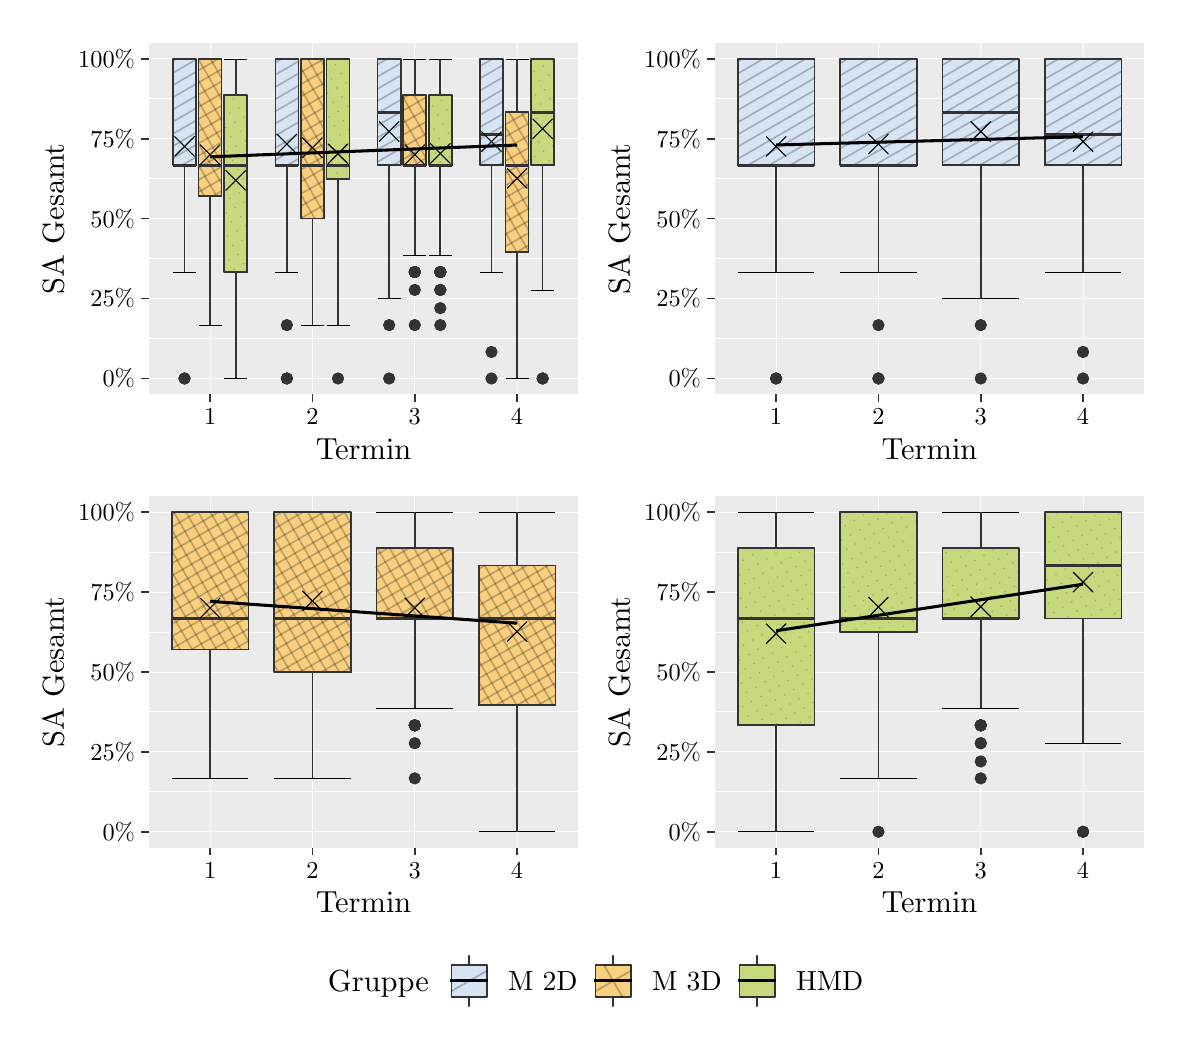
\begin{tikzpicture}[x=1pt,y=1pt]
\definecolor{fillColor}{RGB}{255,255,255}
\path[use as bounding box,fill=fillColor,fill opacity=0.00] (0,0) rectangle (409.05,361.35);
\begin{scope}
\path[clip] (  0.00,197.56) rectangle (204.52,361.35);
\definecolor{drawColor}{RGB}{255,255,255}
\definecolor{fillColor}{RGB}{255,255,255}

\path[draw=drawColor,line width= 0.6pt,line join=round,line cap=round,fill=fillColor] (  0.00,197.56) rectangle (204.52,361.35);
\end{scope}
\begin{scope}
\path[clip] ( 43.73,228.81) rectangle (199.02,355.85);
\definecolor{fillColor}{gray}{0.92}

\path[fill=fillColor] ( 43.73,228.81) rectangle (199.02,355.85);
\definecolor{drawColor}{RGB}{255,255,255}

\path[draw=drawColor,line width= 0.3pt,line join=round] ( 43.73,249.02) --
	(199.02,249.02);

\path[draw=drawColor,line width= 0.3pt,line join=round] ( 43.73,277.89) --
	(199.02,277.89);

\path[draw=drawColor,line width= 0.3pt,line join=round] ( 43.73,306.77) --
	(199.02,306.77);

\path[draw=drawColor,line width= 0.3pt,line join=round] ( 43.73,335.64) --
	(199.02,335.64);

\path[draw=drawColor,line width= 0.3pt,line join=round] ( 43.73,234.58) --
	(199.02,234.58);

\path[draw=drawColor,line width= 0.3pt,line join=round] ( 43.73,263.46) --
	(199.02,263.46);

\path[draw=drawColor,line width= 0.3pt,line join=round] ( 43.73,292.33) --
	(199.02,292.33);

\path[draw=drawColor,line width= 0.3pt,line join=round] ( 43.73,321.20) --
	(199.02,321.20);

\path[draw=drawColor,line width= 0.3pt,line join=round] ( 43.73,350.08) --
	(199.02,350.08);

\path[draw=drawColor,line width= 0.3pt,line join=round] ( 65.92,228.81) --
	( 65.92,355.85);

\path[draw=drawColor,line width= 0.3pt,line join=round] (102.89,228.81) --
	(102.89,355.85);

\path[draw=drawColor,line width= 0.3pt,line join=round] (139.87,228.81) --
	(139.87,355.85);

\path[draw=drawColor,line width= 0.3pt,line join=round] (176.84,228.81) --
	(176.84,355.85);
\definecolor{drawColor}{RGB}{0,0,0}

\path[draw=drawColor,line width= 0.2pt,line join=round] ( 52.51,350.08) --
	( 60.83,350.08);

\path[draw=drawColor,line width= 0.2pt,line join=round] ( 56.67,350.08) --
	( 56.67,273.04);

\path[draw=drawColor,line width= 0.2pt,line join=round] ( 52.51,273.04) --
	( 60.83,273.04);

\path[draw=drawColor,line width= 0.2pt,line join=round] ( 61.76,350.08) --
	( 70.08,350.08);

\path[draw=drawColor,line width= 0.2pt,line join=round] ( 65.92,350.08) --
	( 65.92,253.87);

\path[draw=drawColor,line width= 0.2pt,line join=round] ( 61.76,253.87) --
	( 70.08,253.87);

\path[draw=drawColor,line width= 0.2pt,line join=round] ( 71.00,350.08) --
	( 79.32,350.08);

\path[draw=drawColor,line width= 0.2pt,line join=round] ( 75.16,350.08) --
	( 75.16,234.58);

\path[draw=drawColor,line width= 0.2pt,line join=round] ( 71.00,234.58) --
	( 79.32,234.58);

\path[draw=drawColor,line width= 0.2pt,line join=round] ( 89.49,350.08) --
	( 97.81,350.08);

\path[draw=drawColor,line width= 0.2pt,line join=round] ( 93.65,350.08) --
	( 93.65,273.04);

\path[draw=drawColor,line width= 0.2pt,line join=round] ( 89.49,273.04) --
	( 97.81,273.04);

\path[draw=drawColor,line width= 0.2pt,line join=round] ( 98.73,350.08) --
	(107.05,350.08);

\path[draw=drawColor,line width= 0.2pt,line join=round] (102.89,350.08) --
	(102.89,253.87);

\path[draw=drawColor,line width= 0.2pt,line join=round] ( 98.73,253.87) --
	(107.05,253.87);

\path[draw=drawColor,line width= 0.2pt,line join=round] (107.98,350.08) --
	(116.29,350.08);

\path[draw=drawColor,line width= 0.2pt,line join=round] (112.14,350.08) --
	(112.14,253.87);

\path[draw=drawColor,line width= 0.2pt,line join=round] (107.98,253.87) --
	(116.29,253.87);

\path[draw=drawColor,line width= 0.2pt,line join=round] (126.46,350.08) --
	(134.78,350.08);

\path[draw=drawColor,line width= 0.2pt,line join=round] (130.62,350.08) --
	(130.62,263.46);

\path[draw=drawColor,line width= 0.2pt,line join=round] (126.46,263.46) --
	(134.78,263.46);

\path[draw=drawColor,line width= 0.2pt,line join=round] (135.71,350.08) --
	(144.03,350.08);

\path[draw=drawColor,line width= 0.2pt,line join=round] (139.87,350.08) --
	(139.87,279.28);

\path[draw=drawColor,line width= 0.2pt,line join=round] (135.71,279.28) --
	(144.03,279.28);

\path[draw=drawColor,line width= 0.2pt,line join=round] (144.95,350.08) --
	(153.27,350.08);

\path[draw=drawColor,line width= 0.2pt,line join=round] (149.11,350.08) --
	(149.11,279.28);

\path[draw=drawColor,line width= 0.2pt,line join=round] (144.95,279.28) --
	(153.27,279.28);

\path[draw=drawColor,line width= 0.2pt,line join=round] (163.44,350.08) --
	(171.76,350.08);

\path[draw=drawColor,line width= 0.2pt,line join=round] (167.60,350.08) --
	(167.60,273.04);

\path[draw=drawColor,line width= 0.2pt,line join=round] (163.44,273.04) --
	(171.76,273.04);

\path[draw=drawColor,line width= 0.2pt,line join=round] (172.68,350.08) --
	(181.00,350.08);

\path[draw=drawColor,line width= 0.2pt,line join=round] (176.84,350.08) --
	(176.84,234.58);

\path[draw=drawColor,line width= 0.2pt,line join=round] (172.68,234.58) --
	(181.00,234.58);

\path[draw=drawColor,line width= 0.2pt,line join=round] (181.92,350.08) --
	(190.24,350.08);

\path[draw=drawColor,line width= 0.2pt,line join=round] (186.08,350.08) --
	(186.08,266.58);

\path[draw=drawColor,line width= 0.2pt,line join=round] (181.92,266.58) --
	(190.24,266.58);
\definecolor{drawColor}{gray}{0.20}
\definecolor{fillColor}{gray}{0.20}

\path[draw=drawColor,line width= 0.4pt,line join=round,line cap=round,fill=fillColor] ( 56.67,234.58) circle (  1.96);

\path[draw=drawColor,line width= 0.4pt,line join=round,line cap=round,fill=fillColor] ( 56.67,234.58) circle (  1.96);

\path[draw=drawColor,line width= 0.2pt,line join=round] ( 56.67,350.08) -- ( 56.67,350.08);

\path[draw=drawColor,line width= 0.2pt,line join=round] ( 56.67,311.62) -- ( 56.67,273.04);
\definecolor{fillColor}{RGB}{215,228,244}

\path[draw=drawColor,line width= 0.2pt,fill=fillColor] ( 52.51,350.08) --
	( 52.51,311.62) --
	( 60.83,311.62) --
	( 60.83,350.08) --
	( 52.51,350.08) --
	cycle;

\path[draw=drawColor,line width= 0.5pt] ( 52.51,311.62) -- ( 60.83,311.62);

\path[draw=drawColor,line width= 0.2pt,line join=round] ( 65.92,350.08) -- ( 65.92,350.08);

\path[draw=drawColor,line width= 0.2pt,line join=round] ( 65.92,300.41) -- ( 65.92,253.87);
\definecolor{fillColor}{RGB}{250,208,128}

\path[draw=drawColor,line width= 0.2pt,fill=fillColor] ( 61.76,350.08) --
	( 61.76,300.41) --
	( 70.08,300.41) --
	( 70.08,350.08) --
	( 61.76,350.08) --
	cycle;

\path[draw=drawColor,line width= 0.5pt] ( 61.76,311.62) -- ( 70.08,311.62);

\path[draw=drawColor,line width= 0.2pt,line join=round] ( 75.16,337.02) -- ( 75.16,350.08);

\path[draw=drawColor,line width= 0.2pt,line join=round] ( 75.16,273.04) -- ( 75.16,234.58);
\definecolor{fillColor}{RGB}{199,217,125}

\path[draw=drawColor,line width= 0.2pt,fill=fillColor] ( 71.00,337.02) --
	( 71.00,273.04) --
	( 79.32,273.04) --
	( 79.32,337.02) --
	( 71.00,337.02) --
	cycle;

\path[draw=drawColor,line width= 0.5pt] ( 71.00,311.62) -- ( 79.32,311.62);
\definecolor{fillColor}{gray}{0.20}

\path[draw=drawColor,line width= 0.4pt,line join=round,line cap=round,fill=fillColor] ( 93.65,234.58) circle (  1.96);

\path[draw=drawColor,line width= 0.4pt,line join=round,line cap=round,fill=fillColor] ( 93.65,253.87) circle (  1.96);

\path[draw=drawColor,line width= 0.4pt,line join=round,line cap=round,fill=fillColor] ( 93.65,234.58) circle (  1.96);

\path[draw=drawColor,line width= 0.2pt,line join=round] ( 93.65,350.08) -- ( 93.65,350.08);

\path[draw=drawColor,line width= 0.2pt,line join=round] ( 93.65,311.62) -- ( 93.65,273.04);
\definecolor{fillColor}{RGB}{215,228,244}

\path[draw=drawColor,line width= 0.2pt,fill=fillColor] ( 89.49,350.08) --
	( 89.49,311.62) --
	( 97.81,311.62) --
	( 97.81,350.08) --
	( 89.49,350.08) --
	cycle;

\path[draw=drawColor,line width= 0.5pt] ( 89.49,311.62) -- ( 97.81,311.62);

\path[draw=drawColor,line width= 0.2pt,line join=round] (102.89,350.08) -- (102.89,350.08);

\path[draw=drawColor,line width= 0.2pt,line join=round] (102.89,292.33) -- (102.89,253.87);
\definecolor{fillColor}{RGB}{250,208,128}

\path[draw=drawColor,line width= 0.2pt,fill=fillColor] ( 98.73,350.08) --
	( 98.73,292.33) --
	(107.05,292.33) --
	(107.05,350.08) --
	( 98.73,350.08) --
	cycle;

\path[draw=drawColor,line width= 0.5pt] ( 98.73,311.62) -- (107.05,311.62);
\definecolor{fillColor}{gray}{0.20}

\path[draw=drawColor,line width= 0.4pt,line join=round,line cap=round,fill=fillColor] (112.14,234.58) circle (  1.96);

\path[draw=drawColor,line width= 0.2pt,line join=round] (112.14,350.08) -- (112.14,350.08);

\path[draw=drawColor,line width= 0.2pt,line join=round] (112.14,306.68) -- (112.14,253.87);
\definecolor{fillColor}{RGB}{199,217,125}

\path[draw=drawColor,line width= 0.2pt,fill=fillColor] (107.98,350.08) --
	(107.98,306.68) --
	(116.29,306.68) --
	(116.29,350.08) --
	(107.98,350.08) --
	cycle;

\path[draw=drawColor,line width= 0.5pt] (107.98,311.62) -- (116.29,311.62);
\definecolor{fillColor}{gray}{0.20}

\path[draw=drawColor,line width= 0.4pt,line join=round,line cap=round,fill=fillColor] (130.62,234.58) circle (  1.96);

\path[draw=drawColor,line width= 0.4pt,line join=round,line cap=round,fill=fillColor] (130.62,253.87) circle (  1.96);

\path[draw=drawColor,line width= 0.2pt,line join=round] (130.62,350.08) -- (130.62,350.08);

\path[draw=drawColor,line width= 0.2pt,line join=round] (130.62,311.62) -- (130.62,263.46);
\definecolor{fillColor}{RGB}{215,228,244}

\path[draw=drawColor,line width= 0.2pt,fill=fillColor] (126.46,350.08) --
	(126.46,311.62) --
	(134.78,311.62) --
	(134.78,350.08) --
	(126.46,350.08) --
	cycle;

\path[draw=drawColor,line width= 0.5pt] (126.46,330.79) -- (134.78,330.79);
\definecolor{fillColor}{gray}{0.20}

\path[draw=drawColor,line width= 0.4pt,line join=round,line cap=round,fill=fillColor] (139.87,273.04) circle (  1.96);

\path[draw=drawColor,line width= 0.4pt,line join=round,line cap=round,fill=fillColor] (139.87,273.04) circle (  1.96);

\path[draw=drawColor,line width= 0.4pt,line join=round,line cap=round,fill=fillColor] (139.87,273.04) circle (  1.96);

\path[draw=drawColor,line width= 0.4pt,line join=round,line cap=round,fill=fillColor] (139.87,273.04) circle (  1.96);

\path[draw=drawColor,line width= 0.4pt,line join=round,line cap=round,fill=fillColor] (139.87,266.58) circle (  1.96);

\path[draw=drawColor,line width= 0.4pt,line join=round,line cap=round,fill=fillColor] (139.87,253.87) circle (  1.96);

\path[draw=drawColor,line width= 0.4pt,line join=round,line cap=round,fill=fillColor] (139.87,273.04) circle (  1.96);

\path[draw=drawColor,line width= 0.2pt,line join=round] (139.87,337.02) -- (139.87,350.08);

\path[draw=drawColor,line width= 0.2pt,line join=round] (139.87,311.62) -- (139.87,279.28);
\definecolor{fillColor}{RGB}{250,208,128}

\path[draw=drawColor,line width= 0.2pt,fill=fillColor] (135.71,337.02) --
	(135.71,311.62) --
	(144.03,311.62) --
	(144.03,337.02) --
	(135.71,337.02) --
	cycle;

\path[draw=drawColor,line width= 0.5pt] (135.71,311.62) -- (144.03,311.62);
\definecolor{fillColor}{gray}{0.20}

\path[draw=drawColor,line width= 0.4pt,line join=round,line cap=round,fill=fillColor] (149.11,273.04) circle (  1.96);

\path[draw=drawColor,line width= 0.4pt,line join=round,line cap=round,fill=fillColor] (149.11,273.04) circle (  1.96);

\path[draw=drawColor,line width= 0.4pt,line join=round,line cap=round,fill=fillColor] (149.11,273.04) circle (  1.96);

\path[draw=drawColor,line width= 0.4pt,line join=round,line cap=round,fill=fillColor] (149.11,266.58) circle (  1.96);

\path[draw=drawColor,line width= 0.4pt,line join=round,line cap=round,fill=fillColor] (149.11,259.99) circle (  1.96);

\path[draw=drawColor,line width= 0.4pt,line join=round,line cap=round,fill=fillColor] (149.11,273.04) circle (  1.96);

\path[draw=drawColor,line width= 0.4pt,line join=round,line cap=round,fill=fillColor] (149.11,266.58) circle (  1.96);

\path[draw=drawColor,line width= 0.4pt,line join=round,line cap=round,fill=fillColor] (149.11,253.87) circle (  1.96);

\path[draw=drawColor,line width= 0.4pt,line join=round,line cap=round,fill=fillColor] (149.11,273.04) circle (  1.96);

\path[draw=drawColor,line width= 0.2pt,line join=round] (149.11,337.02) -- (149.11,350.08);

\path[draw=drawColor,line width= 0.2pt,line join=round] (149.11,311.62) -- (149.11,279.28);
\definecolor{fillColor}{RGB}{199,217,125}

\path[draw=drawColor,line width= 0.2pt,fill=fillColor] (144.95,337.02) --
	(144.95,311.62) --
	(153.27,311.62) --
	(153.27,337.02) --
	(144.95,337.02) --
	cycle;

\path[draw=drawColor,line width= 0.5pt] (144.95,311.62) -- (153.27,311.62);
\definecolor{fillColor}{gray}{0.20}

\path[draw=drawColor,line width= 0.4pt,line join=round,line cap=round,fill=fillColor] (167.60,234.58) circle (  1.96);

\path[draw=drawColor,line width= 0.4pt,line join=round,line cap=round,fill=fillColor] (167.60,244.17) circle (  1.96);

\path[draw=drawColor,line width= 0.2pt,line join=round] (167.60,350.08) -- (167.60,350.08);

\path[draw=drawColor,line width= 0.2pt,line join=round] (167.60,311.62) -- (167.60,273.04);
\definecolor{fillColor}{RGB}{215,228,244}

\path[draw=drawColor,line width= 0.2pt,fill=fillColor] (163.44,350.08) --
	(163.44,311.62) --
	(171.76,311.62) --
	(171.76,350.08) --
	(163.44,350.08) --
	cycle;

\path[draw=drawColor,line width= 0.5pt] (163.44,322.70) -- (171.76,322.70);

\path[draw=drawColor,line width= 0.2pt,line join=round] (176.84,330.79) -- (176.84,350.08);

\path[draw=drawColor,line width= 0.2pt,line join=round] (176.84,280.32) -- (176.84,234.58);
\definecolor{fillColor}{RGB}{250,208,128}

\path[draw=drawColor,line width= 0.2pt,fill=fillColor] (172.68,330.79) --
	(172.68,280.32) --
	(181.00,280.32) --
	(181.00,330.79) --
	(172.68,330.79) --
	cycle;

\path[draw=drawColor,line width= 0.5pt] (172.68,311.62) -- (181.00,311.62);
\definecolor{fillColor}{gray}{0.20}

\path[draw=drawColor,line width= 0.4pt,line join=round,line cap=round,fill=fillColor] (186.08,234.58) circle (  1.96);

\path[draw=drawColor,line width= 0.4pt,line join=round,line cap=round,fill=fillColor] (186.08,234.58) circle (  1.96);

\path[draw=drawColor,line width= 0.2pt,line join=round] (186.08,350.08) -- (186.08,350.08);

\path[draw=drawColor,line width= 0.2pt,line join=round] (186.08,311.62) -- (186.08,266.58);
\definecolor{fillColor}{RGB}{199,217,125}

\path[draw=drawColor,line width= 0.2pt,fill=fillColor] (181.92,350.08) --
	(181.92,311.62) --
	(190.24,311.62) --
	(190.24,350.08) --
	(181.92,350.08) --
	cycle;

\path[draw=drawColor,line width= 0.5pt] (181.92,330.79) -- (190.24,330.79);
\definecolor{fillColor}{gray}{0.20}

\path[draw=drawColor,line width= 0.4pt,line join=round,line cap=round,fill=fillColor] ( 56.67,234.58) circle (  1.96);

\path[draw=drawColor,line width= 0.4pt,line join=round,line cap=round,fill=fillColor] ( 56.67,234.58) circle (  1.96);

\path[draw=drawColor,line width= 0.6pt,line join=round] ( 56.67,350.08) -- ( 56.67,350.08);

\path[draw=drawColor,line width= 0.6pt,line join=round] ( 56.67,311.62) -- ( 56.67,273.04);
\definecolor{fillColor}{RGB}{215,228,244}

\path[fill=fillColor] ( 52.51,350.08) --
	( 52.51,311.62) --
	( 60.83,311.62) --
	( 60.83,350.08) --
	( 52.51,350.08) --
	cycle;
\definecolor{drawColor}{RGB}{0,0,0}
\definecolor{fillColor}{RGB}{0,0,0}

\path[draw=drawColor,draw opacity=0.20,line width= 0.6pt,line join=round,line cap=rect,fill=fillColor,fill opacity=0.20] ( 60.83,314.61) --
	( 60.83,314.56) --
	( 55.73,311.62) --
	( 55.66,311.62) --
	( 60.83,314.61) --
	cycle;

\path[draw=drawColor,draw opacity=0.20,line width= 0.6pt,line join=round,line cap=rect,fill=fillColor,fill opacity=0.20] ( 60.83,319.01) --
	( 60.83,318.96) --
	( 52.51,314.16) --
	( 52.51,314.20) --
	( 60.83,319.01) --
	cycle;

\path[draw=drawColor,draw opacity=0.20,line width= 0.6pt,line join=round,line cap=rect,fill=fillColor,fill opacity=0.20] ( 60.83,323.41) --
	( 60.83,323.36) --
	( 52.51,318.56) --
	( 52.51,318.61) --
	( 60.83,323.41) --
	cycle;

\path[draw=drawColor,draw opacity=0.20,line width= 0.6pt,line join=round,line cap=rect,fill=fillColor,fill opacity=0.20] ( 60.83,327.81) --
	( 60.83,327.77) --
	( 52.51,322.96) --
	( 52.51,323.01) --
	( 60.83,327.81) --
	cycle;

\path[draw=drawColor,draw opacity=0.20,line width= 0.6pt,line join=round,line cap=rect,fill=fillColor,fill opacity=0.20] ( 60.83,332.21) --
	( 60.83,332.17) --
	( 52.51,327.36) --
	( 52.51,327.41) --
	( 60.83,332.21) --
	cycle;

\path[draw=drawColor,draw opacity=0.20,line width= 0.6pt,line join=round,line cap=rect,fill=fillColor,fill opacity=0.20] ( 60.83,336.61) --
	( 60.83,336.57) --
	( 52.51,331.76) --
	( 52.51,331.81) --
	( 60.83,336.61) --
	cycle;

\path[draw=drawColor,draw opacity=0.20,line width= 0.6pt,line join=round,line cap=rect,fill=fillColor,fill opacity=0.20] ( 60.83,341.01) --
	( 60.83,340.97) --
	( 52.51,336.16) --
	( 52.51,336.21) --
	( 60.83,341.01) --
	cycle;

\path[draw=drawColor,draw opacity=0.20,line width= 0.6pt,line join=round,line cap=rect,fill=fillColor,fill opacity=0.20] ( 60.83,345.41) --
	( 60.83,345.37) --
	( 52.51,340.57) --
	( 52.51,340.61) --
	( 60.83,345.41) --
	cycle;

\path[draw=drawColor,draw opacity=0.20,line width= 0.6pt,line join=round,line cap=rect,fill=fillColor,fill opacity=0.20] ( 60.83,349.81) --
	( 60.83,349.77) --
	( 52.51,344.97) --
	( 52.51,345.01) --
	( 60.83,349.81) --
	cycle;

\path[draw=drawColor,draw opacity=0.20,line width= 0.6pt,line join=round,line cap=rect,fill=fillColor,fill opacity=0.20] ( 53.67,350.08) --
	( 53.74,350.08) --
	( 52.51,349.37) --
	( 52.51,349.41) --
	( 53.67,350.08) --
	cycle;
\definecolor{drawColor}{gray}{0.20}

\path[draw=drawColor,line width= 0.6pt,line join=round,line cap=round] ( 52.51,350.08) --
	( 52.51,311.62) --
	( 60.83,311.62) --
	( 60.83,350.08) --
	( 52.51,350.08) --
	cycle;

\path[draw=drawColor,line width= 1.1pt,line join=round] ( 52.51,311.62) -- ( 60.83,311.62);
\definecolor{fillColor}{gray}{0.20}

\path[draw=drawColor,line width= 0.4pt,line join=round,line cap=round,fill=fillColor] ( 93.65,234.58) circle (  1.96);

\path[draw=drawColor,line width= 0.4pt,line join=round,line cap=round,fill=fillColor] ( 93.65,253.87) circle (  1.96);

\path[draw=drawColor,line width= 0.4pt,line join=round,line cap=round,fill=fillColor] ( 93.65,234.58) circle (  1.96);

\path[draw=drawColor,line width= 0.6pt,line join=round] ( 93.65,350.08) -- ( 93.65,350.08);

\path[draw=drawColor,line width= 0.6pt,line join=round] ( 93.65,311.62) -- ( 93.65,273.04);
\definecolor{fillColor}{RGB}{215,228,244}

\path[fill=fillColor] ( 89.49,350.08) --
	( 89.49,311.62) --
	( 97.81,311.62) --
	( 97.81,350.08) --
	( 89.49,350.08) --
	cycle;
\definecolor{drawColor}{RGB}{0,0,0}
\definecolor{fillColor}{RGB}{0,0,0}

\path[draw=drawColor,draw opacity=0.20,line width= 0.6pt,line join=round,line cap=rect,fill=fillColor,fill opacity=0.20] ( 97.81,313.95) --
	( 97.81,313.91) --
	( 93.84,311.62) --
	( 93.77,311.62) --
	( 97.81,313.95) --
	cycle;

\path[draw=drawColor,draw opacity=0.20,line width= 0.6pt,line join=round,line cap=rect,fill=fillColor,fill opacity=0.20] ( 97.81,318.35) --
	( 97.81,318.31) --
	( 89.49,313.50) --
	( 89.49,313.55) --
	( 97.81,318.35) --
	cycle;

\path[draw=drawColor,draw opacity=0.20,line width= 0.6pt,line join=round,line cap=rect,fill=fillColor,fill opacity=0.20] ( 97.81,322.75) --
	( 97.81,322.71) --
	( 89.49,317.90) --
	( 89.49,317.95) --
	( 97.81,322.75) --
	cycle;

\path[draw=drawColor,draw opacity=0.20,line width= 0.6pt,line join=round,line cap=rect,fill=fillColor,fill opacity=0.20] ( 97.81,327.15) --
	( 97.81,327.11) --
	( 89.49,322.30) --
	( 89.49,322.35) --
	( 97.81,327.15) --
	cycle;

\path[draw=drawColor,draw opacity=0.20,line width= 0.6pt,line join=round,line cap=rect,fill=fillColor,fill opacity=0.20] ( 97.81,331.55) --
	( 97.81,331.51) --
	( 89.49,326.71) --
	( 89.49,326.75) --
	( 97.81,331.55) --
	cycle;

\path[draw=drawColor,draw opacity=0.20,line width= 0.6pt,line join=round,line cap=rect,fill=fillColor,fill opacity=0.20] ( 97.81,335.95) --
	( 97.81,335.91) --
	( 89.49,331.11) --
	( 89.49,331.15) --
	( 97.81,335.95) --
	cycle;

\path[draw=drawColor,draw opacity=0.20,line width= 0.6pt,line join=round,line cap=rect,fill=fillColor,fill opacity=0.20] ( 97.81,340.35) --
	( 97.81,340.31) --
	( 89.49,335.51) --
	( 89.49,335.55) --
	( 97.81,340.35) --
	cycle;

\path[draw=drawColor,draw opacity=0.20,line width= 0.6pt,line join=round,line cap=rect,fill=fillColor,fill opacity=0.20] ( 97.81,344.76) --
	( 97.81,344.71) --
	( 89.49,339.91) --
	( 89.49,339.95) --
	( 97.81,344.76) --
	cycle;

\path[draw=drawColor,draw opacity=0.20,line width= 0.6pt,line join=round,line cap=rect,fill=fillColor,fill opacity=0.20] ( 97.81,349.16) --
	( 97.81,349.11) --
	( 89.49,344.31) --
	( 89.49,344.35) --
	( 97.81,349.16) --
	cycle;

\path[draw=drawColor,draw opacity=0.20,line width= 0.6pt,line join=round,line cap=rect,fill=fillColor,fill opacity=0.20] ( 91.78,350.08) --
	( 91.85,350.08) --
	( 89.49,348.71) --
	( 89.49,348.75) --
	( 91.78,350.08) --
	cycle;
\definecolor{drawColor}{gray}{0.20}

\path[draw=drawColor,line width= 0.6pt,line join=round,line cap=round] ( 89.49,350.08) --
	( 89.49,311.62) --
	( 97.81,311.62) --
	( 97.81,350.08) --
	( 89.49,350.08) --
	cycle;

\path[draw=drawColor,line width= 1.1pt,line join=round] ( 89.49,311.62) -- ( 97.81,311.62);
\definecolor{fillColor}{gray}{0.20}

\path[draw=drawColor,line width= 0.4pt,line join=round,line cap=round,fill=fillColor] (130.62,234.58) circle (  1.96);

\path[draw=drawColor,line width= 0.4pt,line join=round,line cap=round,fill=fillColor] (130.62,253.87) circle (  1.96);

\path[draw=drawColor,line width= 0.6pt,line join=round] (130.62,350.08) -- (130.62,350.08);

\path[draw=drawColor,line width= 0.6pt,line join=round] (130.62,311.62) -- (130.62,263.46);
\definecolor{fillColor}{RGB}{215,228,244}

\path[fill=fillColor] (126.46,350.08) --
	(126.46,311.62) --
	(134.78,311.62) --
	(134.78,350.08) --
	(126.46,350.08) --
	cycle;
\definecolor{drawColor}{RGB}{0,0,0}
\definecolor{fillColor}{RGB}{0,0,0}

\path[draw=drawColor,draw opacity=0.20,line width= 0.6pt,line join=round,line cap=rect,fill=fillColor,fill opacity=0.20] (134.78,313.29) --
	(134.78,313.25) --
	(131.96,311.62) --
	(131.88,311.62) --
	(134.78,313.29) --
	cycle;

\path[draw=drawColor,draw opacity=0.20,line width= 0.6pt,line join=round,line cap=rect,fill=fillColor,fill opacity=0.20] (134.78,317.69) --
	(134.78,317.65) --
	(126.46,312.85) --
	(126.46,312.89) --
	(134.78,317.69) --
	cycle;

\path[draw=drawColor,draw opacity=0.20,line width= 0.6pt,line join=round,line cap=rect,fill=fillColor,fill opacity=0.20] (134.78,322.09) --
	(134.78,322.05) --
	(126.46,317.25) --
	(126.46,317.29) --
	(134.78,322.09) --
	cycle;

\path[draw=drawColor,draw opacity=0.20,line width= 0.6pt,line join=round,line cap=rect,fill=fillColor,fill opacity=0.20] (134.78,326.49) --
	(134.78,326.45) --
	(126.46,321.65) --
	(126.46,321.69) --
	(134.78,326.49) --
	cycle;

\path[draw=drawColor,draw opacity=0.20,line width= 0.6pt,line join=round,line cap=rect,fill=fillColor,fill opacity=0.20] (134.78,330.90) --
	(134.78,330.85) --
	(126.46,326.05) --
	(126.46,326.09) --
	(134.78,330.90) --
	cycle;

\path[draw=drawColor,draw opacity=0.20,line width= 0.6pt,line join=round,line cap=rect,fill=fillColor,fill opacity=0.20] (134.78,335.30) --
	(134.78,335.25) --
	(126.46,330.45) --
	(126.46,330.49) --
	(134.78,335.30) --
	cycle;

\path[draw=drawColor,draw opacity=0.20,line width= 0.6pt,line join=round,line cap=rect,fill=fillColor,fill opacity=0.20] (134.78,339.70) --
	(134.78,339.65) --
	(126.46,334.85) --
	(126.46,334.89) --
	(134.78,339.70) --
	cycle;

\path[draw=drawColor,draw opacity=0.20,line width= 0.6pt,line join=round,line cap=rect,fill=fillColor,fill opacity=0.20] (134.78,344.10) --
	(134.78,344.05) --
	(126.46,339.25) --
	(126.46,339.30) --
	(134.78,344.10) --
	cycle;

\path[draw=drawColor,draw opacity=0.20,line width= 0.6pt,line join=round,line cap=rect,fill=fillColor,fill opacity=0.20] (134.78,348.50) --
	(134.78,348.45) --
	(126.46,343.65) --
	(126.46,343.70) --
	(134.78,348.50) --
	cycle;

\path[draw=drawColor,draw opacity=0.20,line width= 0.6pt,line join=round,line cap=rect,fill=fillColor,fill opacity=0.20] (129.89,350.08) --
	(129.97,350.08) --
	(126.46,348.05) --
	(126.46,348.10) --
	(129.89,350.08) --
	cycle;
\definecolor{drawColor}{gray}{0.20}

\path[draw=drawColor,line width= 0.6pt,line join=round,line cap=round] (126.46,350.08) --
	(126.46,311.62) --
	(134.78,311.62) --
	(134.78,350.08) --
	(126.46,350.08) --
	cycle;

\path[draw=drawColor,line width= 1.1pt,line join=round] (126.46,330.79) -- (134.78,330.79);
\definecolor{fillColor}{gray}{0.20}

\path[draw=drawColor,line width= 0.4pt,line join=round,line cap=round,fill=fillColor] (167.60,234.58) circle (  1.96);

\path[draw=drawColor,line width= 0.4pt,line join=round,line cap=round,fill=fillColor] (167.60,244.17) circle (  1.96);

\path[draw=drawColor,line width= 0.6pt,line join=round] (167.60,350.08) -- (167.60,350.08);

\path[draw=drawColor,line width= 0.6pt,line join=round] (167.60,311.62) -- (167.60,273.04);
\definecolor{fillColor}{RGB}{215,228,244}

\path[fill=fillColor] (163.44,350.08) --
	(163.44,311.62) --
	(171.76,311.62) --
	(171.76,350.08) --
	(163.44,350.08) --
	cycle;
\definecolor{drawColor}{RGB}{0,0,0}
\definecolor{fillColor}{RGB}{0,0,0}

\path[draw=drawColor,draw opacity=0.20,line width= 0.6pt,line join=round,line cap=rect,fill=fillColor,fill opacity=0.20] (171.76,312.64) --
	(171.76,312.59) --
	(170.07,311.62) --
	(169.99,311.62) --
	(171.76,312.64) --
	cycle;

\path[draw=drawColor,draw opacity=0.20,line width= 0.6pt,line join=round,line cap=rect,fill=fillColor,fill opacity=0.20] (171.76,317.04) --
	(171.76,316.99) --
	(163.44,312.19) --
	(163.44,312.23) --
	(171.76,317.04) --
	cycle;

\path[draw=drawColor,draw opacity=0.20,line width= 0.6pt,line join=round,line cap=rect,fill=fillColor,fill opacity=0.20] (171.76,321.44) --
	(171.76,321.39) --
	(163.44,316.59) --
	(163.44,316.63) --
	(171.76,321.44) --
	cycle;

\path[draw=drawColor,draw opacity=0.20,line width= 0.6pt,line join=round,line cap=rect,fill=fillColor,fill opacity=0.20] (171.76,325.84) --
	(171.76,325.79) --
	(163.44,320.99) --
	(163.44,321.03) --
	(171.76,325.84) --
	cycle;

\path[draw=drawColor,draw opacity=0.20,line width= 0.6pt,line join=round,line cap=rect,fill=fillColor,fill opacity=0.20] (171.76,330.24) --
	(171.76,330.19) --
	(163.44,325.39) --
	(163.44,325.44) --
	(171.76,330.24) --
	cycle;

\path[draw=drawColor,draw opacity=0.20,line width= 0.6pt,line join=round,line cap=rect,fill=fillColor,fill opacity=0.20] (171.76,334.64) --
	(171.76,334.60) --
	(163.44,329.79) --
	(163.44,329.84) --
	(171.76,334.64) --
	cycle;

\path[draw=drawColor,draw opacity=0.20,line width= 0.6pt,line join=round,line cap=rect,fill=fillColor,fill opacity=0.20] (171.76,339.04) --
	(171.76,339.00) --
	(163.44,334.19) --
	(163.44,334.24) --
	(171.76,339.04) --
	cycle;

\path[draw=drawColor,draw opacity=0.20,line width= 0.6pt,line join=round,line cap=rect,fill=fillColor,fill opacity=0.20] (171.76,343.44) --
	(171.76,343.40) --
	(163.44,338.59) --
	(163.44,338.64) --
	(171.76,343.44) --
	cycle;

\path[draw=drawColor,draw opacity=0.20,line width= 0.6pt,line join=round,line cap=rect,fill=fillColor,fill opacity=0.20] (171.76,347.84) --
	(171.76,347.80) --
	(163.44,342.99) --
	(163.44,343.04) --
	(171.76,347.84) --
	cycle;

\path[draw=drawColor,draw opacity=0.20,line width= 0.6pt,line join=round,line cap=rect,fill=fillColor,fill opacity=0.20] (168.00,350.08) --
	(168.08,350.08) --
	(163.44,347.40) --
	(163.44,347.44) --
	(168.00,350.08) --
	cycle;
\definecolor{drawColor}{gray}{0.20}

\path[draw=drawColor,line width= 0.6pt,line join=round,line cap=round] (163.44,350.08) --
	(163.44,311.62) --
	(171.76,311.62) --
	(171.76,350.08) --
	(163.44,350.08) --
	cycle;

\path[draw=drawColor,line width= 1.1pt,line join=round] (163.44,322.70) -- (171.76,322.70);

\path[draw=drawColor,line width= 0.6pt,line join=round] ( 65.92,350.08) -- ( 65.92,350.08);

\path[draw=drawColor,line width= 0.6pt,line join=round] ( 65.92,300.41) -- ( 65.92,253.87);
\definecolor{fillColor}{RGB}{250,208,128}

\path[fill=fillColor] ( 61.76,350.08) --
	( 61.76,300.41) --
	( 70.08,300.41) --
	( 70.08,350.08) --
	( 61.76,350.08) --
	cycle;
\definecolor{drawColor}{RGB}{0,0,0}
\definecolor{fillColor}{RGB}{0,0,0}

\path[draw=drawColor,draw opacity=0.20,line width= 0.6pt,line join=round,line cap=rect,fill=fillColor,fill opacity=0.20] ( 70.08,302.34) --
	( 70.08,302.30) --
	( 66.82,300.41) --
	( 66.74,300.41) --
	( 70.08,302.34) --
	cycle;

\path[draw=drawColor,draw opacity=0.20,line width= 0.6pt,line join=round,line cap=rect,fill=fillColor,fill opacity=0.20] ( 70.08,306.74) --
	( 70.08,306.70) --
	( 61.76,301.89) --
	( 61.76,301.94) --
	( 70.08,306.74) --
	cycle;

\path[draw=drawColor,draw opacity=0.20,line width= 0.6pt,line join=round,line cap=rect,fill=fillColor,fill opacity=0.20] ( 70.08,311.14) --
	( 70.08,311.10) --
	( 61.76,306.29) --
	( 61.76,306.34) --
	( 70.08,311.14) --
	cycle;

\path[draw=drawColor,draw opacity=0.20,line width= 0.6pt,line join=round,line cap=rect,fill=fillColor,fill opacity=0.20] ( 70.08,315.54) --
	( 70.08,315.50) --
	( 61.76,310.70) --
	( 61.76,310.74) --
	( 70.08,315.54) --
	cycle;

\path[draw=drawColor,draw opacity=0.20,line width= 0.6pt,line join=round,line cap=rect,fill=fillColor,fill opacity=0.20] ( 70.08,319.94) --
	( 70.08,319.90) --
	( 61.76,315.10) --
	( 61.76,315.14) --
	( 70.08,319.94) --
	cycle;

\path[draw=drawColor,draw opacity=0.20,line width= 0.6pt,line join=round,line cap=rect,fill=fillColor,fill opacity=0.20] ( 70.08,324.34) --
	( 70.08,324.30) --
	( 61.76,319.50) --
	( 61.76,319.54) --
	( 70.08,324.34) --
	cycle;

\path[draw=drawColor,draw opacity=0.20,line width= 0.6pt,line join=round,line cap=rect,fill=fillColor,fill opacity=0.20] ( 70.08,328.75) --
	( 70.08,328.70) --
	( 61.76,323.90) --
	( 61.76,323.94) --
	( 70.08,328.75) --
	cycle;

\path[draw=drawColor,draw opacity=0.20,line width= 0.6pt,line join=round,line cap=rect,fill=fillColor,fill opacity=0.20] ( 70.08,333.15) --
	( 70.08,333.10) --
	( 61.76,328.30) --
	( 61.76,328.34) --
	( 70.08,333.15) --
	cycle;

\path[draw=drawColor,draw opacity=0.20,line width= 0.6pt,line join=round,line cap=rect,fill=fillColor,fill opacity=0.20] ( 70.08,337.55) --
	( 70.08,337.50) --
	( 61.76,332.70) --
	( 61.76,332.74) --
	( 70.08,337.55) --
	cycle;

\path[draw=drawColor,draw opacity=0.20,line width= 0.6pt,line join=round,line cap=rect,fill=fillColor,fill opacity=0.20] ( 70.08,341.95) --
	( 70.08,341.90) --
	( 61.76,337.10) --
	( 61.76,337.14) --
	( 70.08,341.95) --
	cycle;

\path[draw=drawColor,draw opacity=0.20,line width= 0.6pt,line join=round,line cap=rect,fill=fillColor,fill opacity=0.20] ( 70.08,346.35) --
	( 70.08,346.30) --
	( 61.76,341.50) --
	( 61.76,341.55) --
	( 70.08,346.35) --
	cycle;

\path[draw=drawColor,draw opacity=0.20,line width= 0.6pt,line join=round,line cap=rect,fill=fillColor,fill opacity=0.20] ( 68.91,350.08) --
	( 68.99,350.08) --
	( 61.76,345.90) --
	( 61.76,345.95) --
	( 68.91,350.08) --
	cycle;

\path[draw=drawColor,draw opacity=0.20,line width= 0.6pt,line join=round,line cap=rect,fill=fillColor,fill opacity=0.20] ( 63.92,300.41) --
	( 63.88,300.41) --
	( 61.76,304.09) --
	( 61.76,304.16) --
	( 63.92,300.41) --
	cycle;

\path[draw=drawColor,draw opacity=0.20,line width= 0.6pt,line join=round,line cap=rect,fill=fillColor,fill opacity=0.20] ( 68.32,300.41) --
	( 68.28,300.41) --
	( 61.76,311.71) --
	( 61.76,311.79) --
	( 68.32,300.41) --
	cycle;

\path[draw=drawColor,draw opacity=0.20,line width= 0.6pt,line join=round,line cap=rect,fill=fillColor,fill opacity=0.20] ( 70.08,305.00) --
	( 70.08,304.92) --
	( 61.76,319.33) --
	( 61.76,319.41) --
	( 70.08,305.00) --
	cycle;

\path[draw=drawColor,draw opacity=0.20,line width= 0.6pt,line join=round,line cap=rect,fill=fillColor,fill opacity=0.20] ( 70.08,312.62) --
	( 70.08,312.55) --
	( 61.76,326.96) --
	( 61.76,327.03) --
	( 70.08,312.62) --
	cycle;

\path[draw=drawColor,draw opacity=0.20,line width= 0.6pt,line join=round,line cap=rect,fill=fillColor,fill opacity=0.20] ( 70.08,320.24) --
	( 70.08,320.17) --
	( 61.76,334.58) --
	( 61.76,334.65) --
	( 70.08,320.24) --
	cycle;

\path[draw=drawColor,draw opacity=0.20,line width= 0.6pt,line join=round,line cap=rect,fill=fillColor,fill opacity=0.20] ( 70.08,327.87) --
	( 70.08,327.79) --
	( 61.76,342.20) --
	( 61.76,342.28) --
	( 70.08,327.87) --
	cycle;

\path[draw=drawColor,draw opacity=0.20,line width= 0.6pt,line join=round,line cap=rect,fill=fillColor,fill opacity=0.20] ( 70.08,335.49) --
	( 70.08,335.41) --
	( 61.76,349.82) --
	( 61.76,349.90) --
	( 70.08,335.49) --
	cycle;

\path[draw=drawColor,draw opacity=0.20,line width= 0.6pt,line join=round,line cap=rect,fill=fillColor,fill opacity=0.20] ( 70.08,343.11) --
	( 70.08,343.04) --
	( 66.01,350.08) --
	( 66.06,350.08) --
	( 70.08,343.11) --
	cycle;
\definecolor{drawColor}{gray}{0.20}

\path[draw=drawColor,line width= 0.6pt,line join=round,line cap=round] ( 61.76,350.08) --
	( 61.76,300.41) --
	( 70.08,300.41) --
	( 70.08,350.08) --
	( 61.76,350.08) --
	cycle;

\path[draw=drawColor,line width= 1.1pt,line join=round] ( 61.76,311.62) -- ( 70.08,311.62);

\path[draw=drawColor,line width= 0.6pt,line join=round] (102.89,350.08) -- (102.89,350.08);

\path[draw=drawColor,line width= 0.6pt,line join=round] (102.89,292.33) -- (102.89,253.87);
\definecolor{fillColor}{RGB}{250,208,128}

\path[fill=fillColor] ( 98.73,350.08) --
	( 98.73,292.33) --
	(107.05,292.33) --
	(107.05,350.08) --
	( 98.73,350.08) --
	cycle;
\definecolor{drawColor}{RGB}{0,0,0}
\definecolor{fillColor}{RGB}{0,0,0}

\path[draw=drawColor,draw opacity=0.20,line width= 0.6pt,line join=round,line cap=rect,fill=fillColor,fill opacity=0.20] (107.05,292.88) --
	(107.05,292.84) --
	(106.17,292.33) --
	(106.10,292.33) --
	(107.05,292.88) --
	cycle;

\path[draw=drawColor,draw opacity=0.20,line width= 0.6pt,line join=round,line cap=rect,fill=fillColor,fill opacity=0.20] (107.05,297.28) --
	(107.05,297.24) --
	( 98.73,292.44) --
	( 98.73,292.48) --
	(107.05,297.28) --
	cycle;

\path[draw=drawColor,draw opacity=0.20,line width= 0.6pt,line join=round,line cap=rect,fill=fillColor,fill opacity=0.20] (107.05,301.68) --
	(107.05,301.64) --
	( 98.73,296.84) --
	( 98.73,296.88) --
	(107.05,301.68) --
	cycle;

\path[draw=drawColor,draw opacity=0.20,line width= 0.6pt,line join=round,line cap=rect,fill=fillColor,fill opacity=0.20] (107.05,306.08) --
	(107.05,306.04) --
	( 98.73,301.24) --
	( 98.73,301.28) --
	(107.05,306.08) --
	cycle;

\path[draw=drawColor,draw opacity=0.20,line width= 0.6pt,line join=round,line cap=rect,fill=fillColor,fill opacity=0.20] (107.05,310.48) --
	(107.05,310.44) --
	( 98.73,305.64) --
	( 98.73,305.68) --
	(107.05,310.48) --
	cycle;

\path[draw=drawColor,draw opacity=0.20,line width= 0.6pt,line join=round,line cap=rect,fill=fillColor,fill opacity=0.20] (107.05,314.89) --
	(107.05,314.84) --
	( 98.73,310.04) --
	( 98.73,310.08) --
	(107.05,314.89) --
	cycle;

\path[draw=drawColor,draw opacity=0.20,line width= 0.6pt,line join=round,line cap=rect,fill=fillColor,fill opacity=0.20] (107.05,319.29) --
	(107.05,319.24) --
	( 98.73,314.44) --
	( 98.73,314.48) --
	(107.05,319.29) --
	cycle;

\path[draw=drawColor,draw opacity=0.20,line width= 0.6pt,line join=round,line cap=rect,fill=fillColor,fill opacity=0.20] (107.05,323.69) --
	(107.05,323.64) --
	( 98.73,318.84) --
	( 98.73,318.88) --
	(107.05,323.69) --
	cycle;

\path[draw=drawColor,draw opacity=0.20,line width= 0.6pt,line join=round,line cap=rect,fill=fillColor,fill opacity=0.20] (107.05,328.09) --
	(107.05,328.04) --
	( 98.73,323.24) --
	( 98.73,323.28) --
	(107.05,328.09) --
	cycle;

\path[draw=drawColor,draw opacity=0.20,line width= 0.6pt,line join=round,line cap=rect,fill=fillColor,fill opacity=0.20] (107.05,332.49) --
	(107.05,332.44) --
	( 98.73,327.64) --
	( 98.73,327.69) --
	(107.05,332.49) --
	cycle;

\path[draw=drawColor,draw opacity=0.20,line width= 0.6pt,line join=round,line cap=rect,fill=fillColor,fill opacity=0.20] (107.05,336.89) --
	(107.05,336.85) --
	( 98.73,332.04) --
	( 98.73,332.09) --
	(107.05,336.89) --
	cycle;

\path[draw=drawColor,draw opacity=0.20,line width= 0.6pt,line join=round,line cap=rect,fill=fillColor,fill opacity=0.20] (107.05,341.29) --
	(107.05,341.25) --
	( 98.73,336.44) --
	( 98.73,336.49) --
	(107.05,341.29) --
	cycle;

\path[draw=drawColor,draw opacity=0.20,line width= 0.6pt,line join=round,line cap=rect,fill=fillColor,fill opacity=0.20] (107.05,345.69) --
	(107.05,345.65) --
	( 98.73,340.84) --
	( 98.73,340.89) --
	(107.05,345.69) --
	cycle;

\path[draw=drawColor,draw opacity=0.20,line width= 0.6pt,line join=round,line cap=rect,fill=fillColor,fill opacity=0.20] (107.02,350.08) --
	(107.05,350.08) --
	(107.05,350.05) --
	( 98.73,345.24) --
	( 98.73,345.29) --
	(107.02,350.08) --
	cycle;

\path[draw=drawColor,draw opacity=0.20,line width= 0.6pt,line join=round,line cap=rect,fill=fillColor,fill opacity=0.20] ( 99.40,350.08) --
	( 99.48,350.08) --
	( 98.73,349.65) --
	( 98.73,349.69) --
	( 99.40,350.08) --
	cycle;

\path[draw=drawColor,draw opacity=0.20,line width= 0.6pt,line join=round,line cap=rect,fill=fillColor,fill opacity=0.20] ( 99.40,292.33) --
	( 99.35,292.33) --
	( 98.73,293.40) --
	( 98.73,293.48) --
	( 99.40,292.33) --
	cycle;

\path[draw=drawColor,draw opacity=0.20,line width= 0.6pt,line join=round,line cap=rect,fill=fillColor,fill opacity=0.20] (103.80,292.33) --
	(103.75,292.33) --
	( 98.73,301.03) --
	( 98.73,301.10) --
	(103.80,292.33) --
	cycle;

\path[draw=drawColor,draw opacity=0.20,line width= 0.6pt,line join=round,line cap=rect,fill=fillColor,fill opacity=0.20] (107.05,294.32) --
	(107.05,294.24) --
	( 98.73,308.65) --
	( 98.73,308.73) --
	(107.05,294.32) --
	cycle;

\path[draw=drawColor,draw opacity=0.20,line width= 0.6pt,line join=round,line cap=rect,fill=fillColor,fill opacity=0.20] (107.05,301.94) --
	(107.05,301.86) --
	( 98.73,316.27) --
	( 98.73,316.35) --
	(107.05,301.94) --
	cycle;

\path[draw=drawColor,draw opacity=0.20,line width= 0.6pt,line join=round,line cap=rect,fill=fillColor,fill opacity=0.20] (107.05,309.56) --
	(107.05,309.48) --
	( 98.73,323.89) --
	( 98.73,323.97) --
	(107.05,309.56) --
	cycle;

\path[draw=drawColor,draw opacity=0.20,line width= 0.6pt,line join=round,line cap=rect,fill=fillColor,fill opacity=0.20] (107.05,317.18) --
	(107.05,317.11) --
	( 98.73,331.52) --
	( 98.73,331.59) --
	(107.05,317.18) --
	cycle;

\path[draw=drawColor,draw opacity=0.20,line width= 0.6pt,line join=round,line cap=rect,fill=fillColor,fill opacity=0.20] (107.05,324.81) --
	(107.05,324.73) --
	( 98.73,339.14) --
	( 98.73,339.22) --
	(107.05,324.81) --
	cycle;

\path[draw=drawColor,draw opacity=0.20,line width= 0.6pt,line join=round,line cap=rect,fill=fillColor,fill opacity=0.20] (107.05,332.43) --
	(107.05,332.35) --
	( 98.73,346.76) --
	( 98.73,346.84) --
	(107.05,332.43) --
	cycle;

\path[draw=drawColor,draw opacity=0.20,line width= 0.6pt,line join=round,line cap=rect,fill=fillColor,fill opacity=0.20] (107.05,340.05) --
	(107.05,339.97) --
	(101.22,350.08) --
	(101.26,350.08) --
	(107.05,340.05) --
	cycle;

\path[draw=drawColor,draw opacity=0.20,line width= 0.6pt,line join=round,line cap=rect,fill=fillColor,fill opacity=0.20] (107.05,347.67) --
	(107.05,347.60) --
	(105.62,350.08) --
	(105.66,350.08) --
	(107.05,347.67) --
	cycle;
\definecolor{drawColor}{gray}{0.20}

\path[draw=drawColor,line width= 0.6pt,line join=round,line cap=round] ( 98.73,350.08) --
	( 98.73,292.33) --
	(107.05,292.33) --
	(107.05,350.08) --
	( 98.73,350.08) --
	cycle;

\path[draw=drawColor,line width= 1.1pt,line join=round] ( 98.73,311.62) -- (107.05,311.62);
\definecolor{fillColor}{gray}{0.20}

\path[draw=drawColor,line width= 0.4pt,line join=round,line cap=round,fill=fillColor] (139.87,273.04) circle (  1.96);

\path[draw=drawColor,line width= 0.4pt,line join=round,line cap=round,fill=fillColor] (139.87,273.04) circle (  1.96);

\path[draw=drawColor,line width= 0.4pt,line join=round,line cap=round,fill=fillColor] (139.87,273.04) circle (  1.96);

\path[draw=drawColor,line width= 0.4pt,line join=round,line cap=round,fill=fillColor] (139.87,273.04) circle (  1.96);

\path[draw=drawColor,line width= 0.4pt,line join=round,line cap=round,fill=fillColor] (139.87,266.58) circle (  1.96);

\path[draw=drawColor,line width= 0.4pt,line join=round,line cap=round,fill=fillColor] (139.87,253.87) circle (  1.96);

\path[draw=drawColor,line width= 0.4pt,line join=round,line cap=round,fill=fillColor] (139.87,273.04) circle (  1.96);

\path[draw=drawColor,line width= 0.6pt,line join=round] (139.87,337.02) -- (139.87,350.08);

\path[draw=drawColor,line width= 0.6pt,line join=round] (139.87,311.62) -- (139.87,279.28);
\definecolor{fillColor}{RGB}{250,208,128}

\path[fill=fillColor] (135.71,337.02) --
	(135.71,311.62) --
	(144.03,311.62) --
	(144.03,337.02) --
	(135.71,337.02) --
	cycle;
\definecolor{drawColor}{RGB}{0,0,0}
\definecolor{fillColor}{RGB}{0,0,0}

\path[draw=drawColor,draw opacity=0.20,line width= 0.6pt,line join=round,line cap=rect,fill=fillColor,fill opacity=0.20] (144.03,314.23) --
	(144.03,314.18) --
	(139.58,311.62) --
	(139.50,311.62) --
	(144.03,314.23) --
	cycle;

\path[draw=drawColor,draw opacity=0.20,line width= 0.6pt,line join=round,line cap=rect,fill=fillColor,fill opacity=0.20] (144.03,318.63) --
	(144.03,318.59) --
	(135.71,313.78) --
	(135.71,313.83) --
	(144.03,318.63) --
	cycle;

\path[draw=drawColor,draw opacity=0.20,line width= 0.6pt,line join=round,line cap=rect,fill=fillColor,fill opacity=0.20] (144.03,323.03) --
	(144.03,322.99) --
	(135.71,318.18) --
	(135.71,318.23) --
	(144.03,323.03) --
	cycle;

\path[draw=drawColor,draw opacity=0.20,line width= 0.6pt,line join=round,line cap=rect,fill=fillColor,fill opacity=0.20] (144.03,327.43) --
	(144.03,327.39) --
	(135.71,322.58) --
	(135.71,322.63) --
	(144.03,327.43) --
	cycle;

\path[draw=drawColor,draw opacity=0.20,line width= 0.6pt,line join=round,line cap=rect,fill=fillColor,fill opacity=0.20] (144.03,331.83) --
	(144.03,331.79) --
	(135.71,326.98) --
	(135.71,327.03) --
	(144.03,331.83) --
	cycle;

\path[draw=drawColor,draw opacity=0.20,line width= 0.6pt,line join=round,line cap=rect,fill=fillColor,fill opacity=0.20] (144.03,336.23) --
	(144.03,336.19) --
	(135.71,331.39) --
	(135.71,331.43) --
	(144.03,336.23) --
	cycle;

\path[draw=drawColor,draw opacity=0.20,line width= 0.6pt,line join=round,line cap=rect,fill=fillColor,fill opacity=0.20] (137.78,337.02) --
	(137.85,337.02) --
	(135.71,335.79) --
	(135.71,335.83) --
	(137.78,337.02) --
	cycle;

\path[draw=drawColor,draw opacity=0.20,line width= 0.6pt,line join=round,line cap=rect,fill=fillColor,fill opacity=0.20] (136.67,311.62) --
	(136.63,311.62) --
	(135.71,313.21) --
	(135.71,313.29) --
	(136.67,311.62) --
	cycle;

\path[draw=drawColor,draw opacity=0.20,line width= 0.6pt,line join=round,line cap=rect,fill=fillColor,fill opacity=0.20] (141.07,311.62) --
	(141.03,311.62) --
	(135.71,320.83) --
	(135.71,320.91) --
	(141.07,311.62) --
	cycle;

\path[draw=drawColor,draw opacity=0.20,line width= 0.6pt,line join=round,line cap=rect,fill=fillColor,fill opacity=0.20] (144.03,314.12) --
	(144.03,314.05) --
	(135.71,328.46) --
	(135.71,328.53) --
	(144.03,314.12) --
	cycle;

\path[draw=drawColor,draw opacity=0.20,line width= 0.6pt,line join=round,line cap=rect,fill=fillColor,fill opacity=0.20] (144.03,321.74) --
	(144.03,321.67) --
	(135.71,336.08) --
	(135.71,336.15) --
	(144.03,321.74) --
	cycle;

\path[draw=drawColor,draw opacity=0.20,line width= 0.6pt,line join=round,line cap=rect,fill=fillColor,fill opacity=0.20] (144.03,329.37) --
	(144.03,329.29) --
	(139.56,337.02) --
	(139.60,337.02) --
	(144.03,329.37) --
	cycle;

\path[draw=drawColor,draw opacity=0.20,line width= 0.6pt,line join=round,line cap=rect,fill=fillColor,fill opacity=0.20] (144.03,336.99) --
	(144.03,336.91) --
	(143.96,337.02) --
	(144.00,337.02) --
	(144.03,336.99) --
	cycle;
\definecolor{drawColor}{gray}{0.20}

\path[draw=drawColor,line width= 0.6pt,line join=round,line cap=round] (135.71,337.02) --
	(135.71,311.62) --
	(144.03,311.62) --
	(144.03,337.02) --
	(135.71,337.02) --
	cycle;

\path[draw=drawColor,line width= 1.1pt,line join=round] (135.71,311.62) -- (144.03,311.62);

\path[draw=drawColor,line width= 0.6pt,line join=round] (176.84,330.79) -- (176.84,350.08);

\path[draw=drawColor,line width= 0.6pt,line join=round] (176.84,280.32) -- (176.84,234.58);
\definecolor{fillColor}{RGB}{250,208,128}

\path[fill=fillColor] (172.68,330.79) --
	(172.68,280.32) --
	(181.00,280.32) --
	(181.00,330.79) --
	(172.68,330.79) --
	cycle;
\definecolor{drawColor}{RGB}{0,0,0}
\definecolor{fillColor}{RGB}{0,0,0}

\path[draw=drawColor,draw opacity=0.20,line width= 0.6pt,line join=round,line cap=rect,fill=fillColor,fill opacity=0.20] (181.00,282.77) --
	(181.00,282.72) --
	(176.84,280.32) --
	(176.76,280.32) --
	(181.00,282.77) --
	cycle;

\path[draw=drawColor,draw opacity=0.20,line width= 0.6pt,line join=round,line cap=rect,fill=fillColor,fill opacity=0.20] (181.00,287.17) --
	(181.00,287.12) --
	(172.68,282.32) --
	(172.68,282.36) --
	(181.00,287.17) --
	cycle;

\path[draw=drawColor,draw opacity=0.20,line width= 0.6pt,line join=round,line cap=rect,fill=fillColor,fill opacity=0.20] (181.00,291.57) --
	(181.00,291.52) --
	(172.68,286.72) --
	(172.68,286.76) --
	(181.00,291.57) --
	cycle;

\path[draw=drawColor,draw opacity=0.20,line width= 0.6pt,line join=round,line cap=rect,fill=fillColor,fill opacity=0.20] (181.00,295.97) --
	(181.00,295.92) --
	(172.68,291.12) --
	(172.68,291.16) --
	(181.00,295.97) --
	cycle;

\path[draw=drawColor,draw opacity=0.20,line width= 0.6pt,line join=round,line cap=rect,fill=fillColor,fill opacity=0.20] (181.00,300.37) --
	(181.00,300.32) --
	(172.68,295.52) --
	(172.68,295.57) --
	(181.00,300.37) --
	cycle;

\path[draw=drawColor,draw opacity=0.20,line width= 0.6pt,line join=round,line cap=rect,fill=fillColor,fill opacity=0.20] (181.00,304.77) --
	(181.00,304.73) --
	(172.68,299.92) --
	(172.68,299.97) --
	(181.00,304.77) --
	cycle;

\path[draw=drawColor,draw opacity=0.20,line width= 0.6pt,line join=round,line cap=rect,fill=fillColor,fill opacity=0.20] (181.00,309.17) --
	(181.00,309.13) --
	(172.68,304.32) --
	(172.68,304.37) --
	(181.00,309.17) --
	cycle;

\path[draw=drawColor,draw opacity=0.20,line width= 0.6pt,line join=round,line cap=rect,fill=fillColor,fill opacity=0.20] (181.00,313.57) --
	(181.00,313.53) --
	(172.68,308.72) --
	(172.68,308.77) --
	(181.00,313.57) --
	cycle;

\path[draw=drawColor,draw opacity=0.20,line width= 0.6pt,line join=round,line cap=rect,fill=fillColor,fill opacity=0.20] (181.00,317.97) --
	(181.00,317.93) --
	(172.68,313.12) --
	(172.68,313.17) --
	(181.00,317.97) --
	cycle;

\path[draw=drawColor,draw opacity=0.20,line width= 0.6pt,line join=round,line cap=rect,fill=fillColor,fill opacity=0.20] (181.00,322.37) --
	(181.00,322.33) --
	(172.68,317.53) --
	(172.68,317.57) --
	(181.00,322.37) --
	cycle;

\path[draw=drawColor,draw opacity=0.20,line width= 0.6pt,line join=round,line cap=rect,fill=fillColor,fill opacity=0.20] (181.00,326.77) --
	(181.00,326.73) --
	(172.68,321.93) --
	(172.68,321.97) --
	(181.00,326.77) --
	cycle;

\path[draw=drawColor,draw opacity=0.20,line width= 0.6pt,line join=round,line cap=rect,fill=fillColor,fill opacity=0.20] (180.33,330.79) --
	(180.41,330.79) --
	(172.68,326.33) --
	(172.68,326.37) --
	(180.33,330.79) --
	cycle;

\path[draw=drawColor,draw opacity=0.20,line width= 0.6pt,line join=round,line cap=rect,fill=fillColor,fill opacity=0.20] (172.71,330.79) --
	(172.78,330.79) --
	(172.68,330.73) --
	(172.68,330.77) --
	(172.71,330.79) --
	cycle;

\path[draw=drawColor,draw opacity=0.20,line width= 0.6pt,line join=round,line cap=rect,fill=fillColor,fill opacity=0.20] (176.74,280.32) --
	(176.70,280.32) --
	(172.68,287.28) --
	(172.68,287.36) --
	(176.74,280.32) --
	cycle;

\path[draw=drawColor,draw opacity=0.20,line width= 0.6pt,line join=round,line cap=rect,fill=fillColor,fill opacity=0.20] (181.00,280.57) --
	(181.00,280.50) --
	(172.68,294.90) --
	(172.68,294.98) --
	(181.00,280.57) --
	cycle;

\path[draw=drawColor,draw opacity=0.20,line width= 0.6pt,line join=round,line cap=rect,fill=fillColor,fill opacity=0.20] (181.00,288.19) --
	(181.00,288.12) --
	(172.68,302.53) --
	(172.68,302.60) --
	(181.00,288.19) --
	cycle;

\path[draw=drawColor,draw opacity=0.20,line width= 0.6pt,line join=round,line cap=rect,fill=fillColor,fill opacity=0.20] (181.00,295.82) --
	(181.00,295.74) --
	(172.68,310.15) --
	(172.68,310.23) --
	(181.00,295.82) --
	cycle;

\path[draw=drawColor,draw opacity=0.20,line width= 0.6pt,line join=round,line cap=rect,fill=fillColor,fill opacity=0.20] (181.00,303.44) --
	(181.00,303.36) --
	(172.68,317.77) --
	(172.68,317.85) --
	(181.00,303.44) --
	cycle;

\path[draw=drawColor,draw opacity=0.20,line width= 0.6pt,line join=round,line cap=rect,fill=fillColor,fill opacity=0.20] (181.00,311.06) --
	(181.00,310.98) --
	(172.68,325.39) --
	(172.68,325.47) --
	(181.00,311.06) --
	cycle;

\path[draw=drawColor,draw opacity=0.20,line width= 0.6pt,line join=round,line cap=rect,fill=fillColor,fill opacity=0.20] (181.00,318.68) --
	(181.00,318.61) --
	(173.97,330.79) --
	(174.01,330.79) --
	(181.00,318.68) --
	cycle;

\path[draw=drawColor,draw opacity=0.20,line width= 0.6pt,line join=round,line cap=rect,fill=fillColor,fill opacity=0.20] (181.00,326.31) --
	(181.00,326.23) --
	(178.37,330.79) --
	(178.41,330.79) --
	(181.00,326.31) --
	cycle;
\definecolor{drawColor}{gray}{0.20}

\path[draw=drawColor,line width= 0.6pt,line join=round,line cap=round] (172.68,330.79) --
	(172.68,280.32) --
	(181.00,280.32) --
	(181.00,330.79) --
	(172.68,330.79) --
	cycle;

\path[draw=drawColor,line width= 1.1pt,line join=round] (172.68,311.62) -- (181.00,311.62);

\path[draw=drawColor,line width= 0.6pt,line join=round] ( 75.16,337.02) -- ( 75.16,350.08);

\path[draw=drawColor,line width= 0.6pt,line join=round] ( 75.16,273.04) -- ( 75.16,234.58);
\definecolor{fillColor}{RGB}{199,217,125}

\path[fill=fillColor] ( 71.00,337.02) --
	( 71.00,273.04) --
	( 79.32,273.04) --
	( 79.32,337.02) --
	( 71.00,337.02) --
	cycle;
\definecolor{drawColor}{RGB}{0,0,0}
\definecolor{fillColor}{RGB}{0,0,0}

\path[draw=drawColor,draw opacity=0.20,line width= 0.6pt,line join=round,line cap=round,fill=fillColor,fill opacity=0.20] ( 71.09,333.71) circle (  0.02);

\path[draw=drawColor,draw opacity=0.20,line width= 0.6pt,line join=round,line cap=round,fill=fillColor,fill opacity=0.20] ( 71.22,302.98) circle (  0.02);

\path[draw=drawColor,draw opacity=0.20,line width= 0.6pt,line join=round,line cap=round,fill=fillColor,fill opacity=0.20] ( 71.60,325.20) circle (  0.02);

\path[draw=drawColor,draw opacity=0.20,line width= 0.6pt,line join=round,line cap=round,fill=fillColor,fill opacity=0.20] ( 71.73,294.47) circle (  0.02);

\path[draw=drawColor,draw opacity=0.20,line width= 0.6pt,line join=round,line cap=round,fill=fillColor,fill opacity=0.20] ( 72.11,316.69) circle (  0.02);

\path[draw=drawColor,draw opacity=0.20,line width= 0.6pt,line join=round,line cap=round,fill=fillColor,fill opacity=0.20] ( 72.24,285.97) circle (  0.02);

\path[draw=drawColor,draw opacity=0.20,line width= 0.6pt,line join=round,line cap=round,fill=fillColor,fill opacity=0.20] ( 72.62,308.19) circle (  0.02);

\path[draw=drawColor,draw opacity=0.20,line width= 0.6pt,line join=round,line cap=round,fill=fillColor,fill opacity=0.20] ( 72.75,277.46) circle (  0.02);

\path[draw=drawColor,draw opacity=0.20,line width= 0.6pt,line join=round,line cap=round,fill=fillColor,fill opacity=0.20] ( 72.99,330.41) circle (  0.02);

\path[draw=drawColor,draw opacity=0.20,line width= 0.6pt,line join=round,line cap=round,fill=fillColor,fill opacity=0.20] ( 73.13,299.68) circle (  0.02);

\path[draw=drawColor,draw opacity=0.20,line width= 0.6pt,line join=round,line cap=round,fill=fillColor,fill opacity=0.20] ( 73.50,321.90) circle (  0.02);

\path[draw=drawColor,draw opacity=0.20,line width= 0.6pt,line join=round,line cap=round,fill=fillColor,fill opacity=0.20] ( 73.64,291.17) circle (  0.02);

\path[draw=drawColor,draw opacity=0.20,line width= 0.6pt,line join=round,line cap=round,fill=fillColor,fill opacity=0.20] ( 74.01,313.39) circle (  0.02);

\path[draw=drawColor,draw opacity=0.20,line width= 0.6pt,line join=round,line cap=round,fill=fillColor,fill opacity=0.20] ( 74.15,282.66) circle (  0.02);

\path[draw=drawColor,draw opacity=0.20,line width= 0.6pt,line join=round,line cap=round,fill=fillColor,fill opacity=0.20] ( 74.39,335.61) circle (  0.02);

\path[draw=drawColor,draw opacity=0.20,line width= 0.6pt,line join=round,line cap=round,fill=fillColor,fill opacity=0.20] ( 74.52,304.88) circle (  0.02);

\path[draw=drawColor,draw opacity=0.20,line width= 0.6pt,line join=round,line cap=round,fill=fillColor,fill opacity=0.20] ( 74.66,274.16) circle (  0.02);

\path[draw=drawColor,draw opacity=0.20,line width= 0.6pt,line join=round,line cap=round,fill=fillColor,fill opacity=0.20] ( 74.90,327.10) circle (  0.02);

\path[draw=drawColor,draw opacity=0.20,line width= 0.6pt,line join=round,line cap=round,fill=fillColor,fill opacity=0.20] ( 75.03,296.38) circle (  0.02);

\path[draw=drawColor,draw opacity=0.20,line width= 0.6pt,line join=round,line cap=round,fill=fillColor,fill opacity=0.20] ( 75.41,318.60) circle (  0.02);

\path[draw=drawColor,draw opacity=0.20,line width= 0.6pt,line join=round,line cap=round,fill=fillColor,fill opacity=0.20] ( 75.54,287.87) circle (  0.02);

\path[draw=drawColor,draw opacity=0.20,line width= 0.6pt,line join=round,line cap=round,fill=fillColor,fill opacity=0.20] ( 75.92,310.09) circle (  0.02);

\path[draw=drawColor,draw opacity=0.20,line width= 0.6pt,line join=round,line cap=round,fill=fillColor,fill opacity=0.20] ( 76.05,279.36) circle (  0.02);

\path[draw=drawColor,draw opacity=0.20,line width= 0.6pt,line join=round,line cap=round,fill=fillColor,fill opacity=0.20] ( 76.29,332.31) circle (  0.02);

\path[draw=drawColor,draw opacity=0.20,line width= 0.6pt,line join=round,line cap=round,fill=fillColor,fill opacity=0.20] ( 76.43,301.58) circle (  0.02);

\path[draw=drawColor,draw opacity=0.20,line width= 0.6pt,line join=round,line cap=round,fill=fillColor,fill opacity=0.20] ( 76.80,323.80) circle (  0.02);

\path[draw=drawColor,draw opacity=0.20,line width= 0.6pt,line join=round,line cap=round,fill=fillColor,fill opacity=0.20] ( 76.94,293.08) circle (  0.02);

\path[draw=drawColor,draw opacity=0.20,line width= 0.6pt,line join=round,line cap=round,fill=fillColor,fill opacity=0.20] ( 77.31,315.30) circle (  0.02);

\path[draw=drawColor,draw opacity=0.20,line width= 0.6pt,line join=round,line cap=round,fill=fillColor,fill opacity=0.20] ( 77.45,284.57) circle (  0.02);

\path[draw=drawColor,draw opacity=0.20,line width= 0.6pt,line join=round,line cap=round,fill=fillColor,fill opacity=0.20] ( 77.82,306.79) circle (  0.02);

\path[draw=drawColor,draw opacity=0.20,line width= 0.6pt,line join=round,line cap=round,fill=fillColor,fill opacity=0.20] ( 77.96,276.06) circle (  0.02);

\path[draw=drawColor,draw opacity=0.20,line width= 0.6pt,line join=round,line cap=round,fill=fillColor,fill opacity=0.20] ( 78.20,329.01) circle (  0.02);

\path[draw=drawColor,draw opacity=0.20,line width= 0.6pt,line join=round,line cap=round,fill=fillColor,fill opacity=0.20] ( 78.33,298.28) circle (  0.02);

\path[draw=drawColor,draw opacity=0.20,line width= 0.6pt,line join=round,line cap=round,fill=fillColor,fill opacity=0.20] ( 78.71,320.50) circle (  0.02);

\path[draw=drawColor,draw opacity=0.20,line width= 0.6pt,line join=round,line cap=round,fill=fillColor,fill opacity=0.20] ( 78.84,289.78) circle (  0.02);

\path[draw=drawColor,draw opacity=0.20,line width= 0.6pt,line join=round,line cap=round,fill=fillColor,fill opacity=0.20] ( 79.22,312.00) circle (  0.02);
\definecolor{drawColor}{gray}{0.20}

\path[draw=drawColor,line width= 0.6pt,line join=round,line cap=round] ( 71.00,337.02) --
	( 71.00,273.04) --
	( 79.32,273.04) --
	( 79.32,337.02) --
	( 71.00,337.02) --
	cycle;

\path[draw=drawColor,line width= 1.1pt,line join=round] ( 71.00,311.62) -- ( 79.32,311.62);
\definecolor{fillColor}{gray}{0.20}

\path[draw=drawColor,line width= 0.4pt,line join=round,line cap=round,fill=fillColor] (112.14,234.58) circle (  1.96);

\path[draw=drawColor,line width= 0.6pt,line join=round] (112.14,350.08) -- (112.14,350.08);

\path[draw=drawColor,line width= 0.6pt,line join=round] (112.14,306.68) -- (112.14,253.87);
\definecolor{fillColor}{RGB}{199,217,125}

\path[fill=fillColor] (107.98,350.08) --
	(107.98,306.68) --
	(116.29,306.68) --
	(116.29,350.08) --
	(107.98,350.08) --
	cycle;
\definecolor{drawColor}{RGB}{0,0,0}
\definecolor{fillColor}{RGB}{0,0,0}

\path[draw=drawColor,draw opacity=0.20,line width= 0.6pt,line join=round,line cap=round,fill=fillColor,fill opacity=0.20] (108.04,315.43) circle (  0.02);

\path[draw=drawColor,draw opacity=0.20,line width= 0.6pt,line join=round,line cap=round,fill=fillColor,fill opacity=0.20] (108.41,337.65) circle (  0.02);

\path[draw=drawColor,draw opacity=0.20,line width= 0.6pt,line join=round,line cap=round,fill=fillColor,fill opacity=0.20] (108.55,306.93) circle (  0.02);

\path[draw=drawColor,draw opacity=0.20,line width= 0.6pt,line join=round,line cap=round,fill=fillColor,fill opacity=0.20] (108.92,329.15) circle (  0.02);

\path[draw=drawColor,draw opacity=0.20,line width= 0.6pt,line join=round,line cap=round,fill=fillColor,fill opacity=0.20] (109.43,320.64) circle (  0.02);

\path[draw=drawColor,draw opacity=0.20,line width= 0.6pt,line join=round,line cap=round,fill=fillColor,fill opacity=0.20] (109.81,342.86) circle (  0.02);

\path[draw=drawColor,draw opacity=0.20,line width= 0.6pt,line join=round,line cap=round,fill=fillColor,fill opacity=0.20] (109.95,312.13) circle (  0.02);

\path[draw=drawColor,draw opacity=0.20,line width= 0.6pt,line join=round,line cap=round,fill=fillColor,fill opacity=0.20] (110.32,334.35) circle (  0.02);

\path[draw=drawColor,draw opacity=0.20,line width= 0.6pt,line join=round,line cap=round,fill=fillColor,fill opacity=0.20] (110.83,325.85) circle (  0.02);

\path[draw=drawColor,draw opacity=0.20,line width= 0.6pt,line join=round,line cap=round,fill=fillColor,fill opacity=0.20] (111.20,348.07) circle (  0.02);

\path[draw=drawColor,draw opacity=0.20,line width= 0.6pt,line join=round,line cap=round,fill=fillColor,fill opacity=0.20] (111.34,317.34) circle (  0.02);

\path[draw=drawColor,draw opacity=0.20,line width= 0.6pt,line join=round,line cap=round,fill=fillColor,fill opacity=0.20] (111.71,339.56) circle (  0.02);

\path[draw=drawColor,draw opacity=0.20,line width= 0.6pt,line join=round,line cap=round,fill=fillColor,fill opacity=0.20] (111.85,308.83) circle (  0.02);

\path[draw=drawColor,draw opacity=0.20,line width= 0.6pt,line join=round,line cap=round,fill=fillColor,fill opacity=0.20] (112.22,331.05) circle (  0.02);

\path[draw=drawColor,draw opacity=0.20,line width= 0.6pt,line join=round,line cap=round,fill=fillColor,fill opacity=0.20] (112.74,322.55) circle (  0.02);

\path[draw=drawColor,draw opacity=0.20,line width= 0.6pt,line join=round,line cap=round,fill=fillColor,fill opacity=0.20] (113.11,344.77) circle (  0.02);

\path[draw=drawColor,draw opacity=0.20,line width= 0.6pt,line join=round,line cap=round,fill=fillColor,fill opacity=0.20] (113.25,314.04) circle (  0.02);

\path[draw=drawColor,draw opacity=0.20,line width= 0.6pt,line join=round,line cap=round,fill=fillColor,fill opacity=0.20] (113.62,336.26) circle (  0.02);

\path[draw=drawColor,draw opacity=0.20,line width= 0.6pt,line join=round,line cap=round,fill=fillColor,fill opacity=0.20] (114.13,327.75) circle (  0.02);

\path[draw=drawColor,draw opacity=0.20,line width= 0.6pt,line join=round,line cap=round,fill=fillColor,fill opacity=0.20] (114.50,349.97) circle (  0.02);

\path[draw=drawColor,draw opacity=0.20,line width= 0.6pt,line join=round,line cap=round,fill=fillColor,fill opacity=0.20] (114.64,319.25) circle (  0.02);

\path[draw=drawColor,draw opacity=0.20,line width= 0.6pt,line join=round,line cap=round,fill=fillColor,fill opacity=0.20] (115.01,341.47) circle (  0.02);

\path[draw=drawColor,draw opacity=0.20,line width= 0.6pt,line join=round,line cap=round,fill=fillColor,fill opacity=0.20] (115.15,310.74) circle (  0.02);

\path[draw=drawColor,draw opacity=0.20,line width= 0.6pt,line join=round,line cap=round,fill=fillColor,fill opacity=0.20] (115.53,332.96) circle (  0.02);

\path[draw=drawColor,draw opacity=0.20,line width= 0.6pt,line join=round,line cap=round,fill=fillColor,fill opacity=0.20] (116.04,324.45) circle (  0.02);
\definecolor{drawColor}{gray}{0.20}

\path[draw=drawColor,line width= 0.6pt,line join=round,line cap=round] (107.98,350.08) --
	(107.98,306.68) --
	(116.29,306.68) --
	(116.29,350.08) --
	(107.98,350.08) --
	cycle;

\path[draw=drawColor,line width= 1.1pt,line join=round] (107.98,311.62) -- (116.29,311.62);
\definecolor{fillColor}{gray}{0.20}

\path[draw=drawColor,line width= 0.4pt,line join=round,line cap=round,fill=fillColor] (149.11,273.04) circle (  1.96);

\path[draw=drawColor,line width= 0.4pt,line join=round,line cap=round,fill=fillColor] (149.11,273.04) circle (  1.96);

\path[draw=drawColor,line width= 0.4pt,line join=round,line cap=round,fill=fillColor] (149.11,273.04) circle (  1.96);

\path[draw=drawColor,line width= 0.4pt,line join=round,line cap=round,fill=fillColor] (149.11,266.58) circle (  1.96);

\path[draw=drawColor,line width= 0.4pt,line join=round,line cap=round,fill=fillColor] (149.11,259.99) circle (  1.96);

\path[draw=drawColor,line width= 0.4pt,line join=round,line cap=round,fill=fillColor] (149.11,273.04) circle (  1.96);

\path[draw=drawColor,line width= 0.4pt,line join=round,line cap=round,fill=fillColor] (149.11,266.58) circle (  1.96);

\path[draw=drawColor,line width= 0.4pt,line join=round,line cap=round,fill=fillColor] (149.11,253.87) circle (  1.96);

\path[draw=drawColor,line width= 0.4pt,line join=round,line cap=round,fill=fillColor] (149.11,273.04) circle (  1.96);

\path[draw=drawColor,line width= 0.6pt,line join=round] (149.11,337.02) -- (149.11,350.08);

\path[draw=drawColor,line width= 0.6pt,line join=round] (149.11,311.62) -- (149.11,279.28);
\definecolor{fillColor}{RGB}{199,217,125}

\path[fill=fillColor] (144.95,337.02) --
	(144.95,311.62) --
	(153.27,311.62) --
	(153.27,337.02) --
	(144.95,337.02) --
	cycle;
\definecolor{drawColor}{RGB}{0,0,0}
\definecolor{fillColor}{RGB}{0,0,0}

\path[draw=drawColor,draw opacity=0.20,line width= 0.6pt,line join=round,line cap=round,fill=fillColor,fill opacity=0.20] (145.37,319.38) circle (  0.02);

\path[draw=drawColor,draw opacity=0.20,line width= 0.6pt,line join=round,line cap=round,fill=fillColor,fill opacity=0.20] (146.25,333.10) circle (  0.02);

\path[draw=drawColor,draw opacity=0.20,line width= 0.6pt,line join=round,line cap=round,fill=fillColor,fill opacity=0.20] (146.76,324.59) circle (  0.02);

\path[draw=drawColor,draw opacity=0.20,line width= 0.6pt,line join=round,line cap=round,fill=fillColor,fill opacity=0.20] (147.27,316.08) circle (  0.02);

\path[draw=drawColor,draw opacity=0.20,line width= 0.6pt,line join=round,line cap=round,fill=fillColor,fill opacity=0.20] (148.16,329.79) circle (  0.02);

\path[draw=drawColor,draw opacity=0.20,line width= 0.6pt,line join=round,line cap=round,fill=fillColor,fill opacity=0.20] (148.67,321.29) circle (  0.02);

\path[draw=drawColor,draw opacity=0.20,line width= 0.6pt,line join=round,line cap=round,fill=fillColor,fill opacity=0.20] (149.18,312.78) circle (  0.02);

\path[draw=drawColor,draw opacity=0.20,line width= 0.6pt,line join=round,line cap=round,fill=fillColor,fill opacity=0.20] (149.55,335.00) circle (  0.02);

\path[draw=drawColor,draw opacity=0.20,line width= 0.6pt,line join=round,line cap=round,fill=fillColor,fill opacity=0.20] (150.06,326.49) circle (  0.02);

\path[draw=drawColor,draw opacity=0.20,line width= 0.6pt,line join=round,line cap=round,fill=fillColor,fill opacity=0.20] (150.57,317.99) circle (  0.02);

\path[draw=drawColor,draw opacity=0.20,line width= 0.6pt,line join=round,line cap=round,fill=fillColor,fill opacity=0.20] (151.46,331.70) circle (  0.02);

\path[draw=drawColor,draw opacity=0.20,line width= 0.6pt,line join=round,line cap=round,fill=fillColor,fill opacity=0.20] (151.97,323.19) circle (  0.02);

\path[draw=drawColor,draw opacity=0.20,line width= 0.6pt,line join=round,line cap=round,fill=fillColor,fill opacity=0.20] (152.48,314.69) circle (  0.02);

\path[draw=drawColor,draw opacity=0.20,line width= 0.6pt,line join=round,line cap=round,fill=fillColor,fill opacity=0.20] (152.85,336.91) circle (  0.02);
\definecolor{drawColor}{gray}{0.20}

\path[draw=drawColor,line width= 0.6pt,line join=round,line cap=round] (144.95,337.02) --
	(144.95,311.62) --
	(153.27,311.62) --
	(153.27,337.02) --
	(144.95,337.02) --
	cycle;

\path[draw=drawColor,line width= 1.1pt,line join=round] (144.95,311.62) -- (153.27,311.62);
\definecolor{fillColor}{gray}{0.20}

\path[draw=drawColor,line width= 0.4pt,line join=round,line cap=round,fill=fillColor] (186.08,234.58) circle (  1.96);

\path[draw=drawColor,line width= 0.4pt,line join=round,line cap=round,fill=fillColor] (186.08,234.58) circle (  1.96);

\path[draw=drawColor,line width= 0.6pt,line join=round] (186.08,350.08) -- (186.08,350.08);

\path[draw=drawColor,line width= 0.6pt,line join=round] (186.08,311.62) -- (186.08,266.58);
\definecolor{fillColor}{RGB}{199,217,125}

\path[fill=fillColor] (181.92,350.08) --
	(181.92,311.62) --
	(190.24,311.62) --
	(190.24,350.08) --
	(181.92,350.08) --
	cycle;
\definecolor{drawColor}{RGB}{0,0,0}
\definecolor{fillColor}{RGB}{0,0,0}

\path[draw=drawColor,draw opacity=0.20,line width= 0.6pt,line join=round,line cap=round,fill=fillColor,fill opacity=0.20] (182.18,331.84) circle (  0.02);

\path[draw=drawColor,draw opacity=0.20,line width= 0.6pt,line join=round,line cap=round,fill=fillColor,fill opacity=0.20] (182.70,323.33) circle (  0.02);

\path[draw=drawColor,draw opacity=0.20,line width= 0.6pt,line join=round,line cap=round,fill=fillColor,fill opacity=0.20] (183.07,345.55) circle (  0.02);

\path[draw=drawColor,draw opacity=0.20,line width= 0.6pt,line join=round,line cap=round,fill=fillColor,fill opacity=0.20] (183.21,314.82) circle (  0.02);

\path[draw=drawColor,draw opacity=0.20,line width= 0.6pt,line join=round,line cap=round,fill=fillColor,fill opacity=0.20] (183.58,337.04) circle (  0.02);

\path[draw=drawColor,draw opacity=0.20,line width= 0.6pt,line join=round,line cap=round,fill=fillColor,fill opacity=0.20] (184.09,328.54) circle (  0.02);

\path[draw=drawColor,draw opacity=0.20,line width= 0.6pt,line join=round,line cap=round,fill=fillColor,fill opacity=0.20] (184.60,320.03) circle (  0.02);

\path[draw=drawColor,draw opacity=0.20,line width= 0.6pt,line join=round,line cap=round,fill=fillColor,fill opacity=0.20] (184.97,342.25) circle (  0.02);

\path[draw=drawColor,draw opacity=0.20,line width= 0.6pt,line join=round,line cap=round,fill=fillColor,fill opacity=0.20] (185.49,333.74) circle (  0.02);

\path[draw=drawColor,draw opacity=0.20,line width= 0.6pt,line join=round,line cap=round,fill=fillColor,fill opacity=0.20] (186.00,325.24) circle (  0.02);

\path[draw=drawColor,draw opacity=0.20,line width= 0.6pt,line join=round,line cap=round,fill=fillColor,fill opacity=0.20] (186.37,347.46) circle (  0.02);

\path[draw=drawColor,draw opacity=0.20,line width= 0.6pt,line join=round,line cap=round,fill=fillColor,fill opacity=0.20] (186.51,316.73) circle (  0.02);

\path[draw=drawColor,draw opacity=0.20,line width= 0.6pt,line join=round,line cap=round,fill=fillColor,fill opacity=0.20] (186.88,338.95) circle (  0.02);

\path[draw=drawColor,draw opacity=0.20,line width= 0.6pt,line join=round,line cap=round,fill=fillColor,fill opacity=0.20] (187.39,330.44) circle (  0.02);

\path[draw=drawColor,draw opacity=0.20,line width= 0.6pt,line join=round,line cap=round,fill=fillColor,fill opacity=0.20] (187.90,321.94) circle (  0.02);

\path[draw=drawColor,draw opacity=0.20,line width= 0.6pt,line join=round,line cap=round,fill=fillColor,fill opacity=0.20] (188.28,344.15) circle (  0.02);

\path[draw=drawColor,draw opacity=0.20,line width= 0.6pt,line join=round,line cap=round,fill=fillColor,fill opacity=0.20] (188.41,313.43) circle (  0.02);

\path[draw=drawColor,draw opacity=0.20,line width= 0.6pt,line join=round,line cap=round,fill=fillColor,fill opacity=0.20] (188.79,335.65) circle (  0.02);

\path[draw=drawColor,draw opacity=0.20,line width= 0.6pt,line join=round,line cap=round,fill=fillColor,fill opacity=0.20] (189.30,327.14) circle (  0.02);

\path[draw=drawColor,draw opacity=0.20,line width= 0.6pt,line join=round,line cap=round,fill=fillColor,fill opacity=0.20] (189.67,349.36) circle (  0.02);

\path[draw=drawColor,draw opacity=0.20,line width= 0.6pt,line join=round,line cap=round,fill=fillColor,fill opacity=0.20] (189.81,318.63) circle (  0.02);

\path[draw=drawColor,draw opacity=0.20,line width= 0.6pt,line join=round,line cap=round,fill=fillColor,fill opacity=0.20] (190.18,340.85) circle (  0.02);
\definecolor{drawColor}{gray}{0.20}

\path[draw=drawColor,line width= 0.6pt,line join=round,line cap=round] (181.92,350.08) --
	(181.92,311.62) --
	(190.24,311.62) --
	(190.24,350.08) --
	(181.92,350.08) --
	cycle;

\path[draw=drawColor,line width= 1.1pt,line join=round] (181.92,330.79) -- (190.24,330.79);
\definecolor{drawColor}{RGB}{0,0,0}

\path[draw=drawColor,line width= 0.4pt,line join=round,line cap=round] ( 53.11,314.86) -- ( 60.24,321.99);

\path[draw=drawColor,line width= 0.4pt,line join=round,line cap=round] ( 53.11,321.99) -- ( 60.24,314.86);

\path[draw=drawColor,line width= 0.4pt,line join=round,line cap=round] ( 62.35,311.86) -- ( 69.49,318.99);

\path[draw=drawColor,line width= 0.4pt,line join=round,line cap=round] ( 62.35,318.99) -- ( 69.49,311.86);

\path[draw=drawColor,line width= 0.4pt,line join=round,line cap=round] ( 71.59,302.60) -- ( 78.73,309.74);

\path[draw=drawColor,line width= 0.4pt,line join=round,line cap=round] ( 71.59,309.74) -- ( 78.73,302.60);

\path[draw=drawColor,line width= 0.4pt,line join=round,line cap=round] ( 90.08,315.74) -- ( 97.22,322.88);

\path[draw=drawColor,line width= 0.4pt,line join=round,line cap=round] ( 90.08,322.88) -- ( 97.22,315.74);

\path[draw=drawColor,line width= 0.4pt,line join=round,line cap=round] ( 99.32,314.42) -- (106.46,321.56);

\path[draw=drawColor,line width= 0.4pt,line join=round,line cap=round] ( 99.32,321.56) -- (106.46,314.42);

\path[draw=drawColor,line width= 0.4pt,line join=round,line cap=round] (108.57,312.21) -- (115.70,319.35);

\path[draw=drawColor,line width= 0.4pt,line join=round,line cap=round] (108.57,319.35) -- (115.70,312.21);

\path[draw=drawColor,line width= 0.4pt,line join=round,line cap=round] (127.05,320.26) -- (134.19,327.40);

\path[draw=drawColor,line width= 0.4pt,line join=round,line cap=round] (127.05,327.40) -- (134.19,320.26);

\path[draw=drawColor,line width= 0.4pt,line join=round,line cap=round] (136.30,311.90) -- (143.43,319.04);

\path[draw=drawColor,line width= 0.4pt,line join=round,line cap=round] (136.30,319.04) -- (143.43,311.90);

\path[draw=drawColor,line width= 0.4pt,line join=round,line cap=round] (145.54,312.32) -- (152.68,319.46);

\path[draw=drawColor,line width= 0.4pt,line join=round,line cap=round] (145.54,319.46) -- (152.68,312.32);

\path[draw=drawColor,line width= 0.4pt,line join=round,line cap=round] (164.03,316.62) -- (171.16,323.76);

\path[draw=drawColor,line width= 0.4pt,line join=round,line cap=round] (164.03,323.76) -- (171.16,316.62);

\path[draw=drawColor,line width= 0.4pt,line join=round,line cap=round] (173.27,303.33) -- (180.41,310.47);

\path[draw=drawColor,line width= 0.4pt,line join=round,line cap=round] (173.27,310.47) -- (180.41,303.33);

\path[draw=drawColor,line width= 0.4pt,line join=round,line cap=round] (182.51,321.24) -- (189.65,328.37);

\path[draw=drawColor,line width= 0.4pt,line join=round,line cap=round] (182.51,328.37) -- (189.65,321.24);

\path[draw=drawColor,line width= 1.1pt,line join=round] ( 65.92,314.69) --
	( 67.32,314.74) --
	( 68.73,314.79) --
	( 70.13,314.85) --
	( 71.53,314.90) --
	( 72.94,314.95) --
	( 74.34,315.01) --
	( 75.75,315.06) --
	( 77.15,315.12) --
	( 78.55,315.17) --
	( 79.96,315.22) --
	( 81.36,315.28) --
	( 82.77,315.33) --
	( 84.17,315.39) --
	( 85.57,315.44) --
	( 86.98,315.49) --
	( 88.38,315.55) --
	( 89.79,315.60) --
	( 91.19,315.65) --
	( 92.60,315.71) --
	( 94.00,315.76) --
	( 95.40,315.82) --
	( 96.81,315.87) --
	( 98.21,315.92) --
	( 99.62,315.98) --
	(101.02,316.03) --
	(102.42,316.08) --
	(103.83,316.14) --
	(105.23,316.19) --
	(106.64,316.25) --
	(108.04,316.30) --
	(109.44,316.35) --
	(110.85,316.41) --
	(112.25,316.46) --
	(113.66,316.52) --
	(115.06,316.57) --
	(116.46,316.62) --
	(117.87,316.68) --
	(119.27,316.73) --
	(120.68,316.78) --
	(122.08,316.84) --
	(123.48,316.89) --
	(124.89,316.95) --
	(126.29,317.00) --
	(127.70,317.05) --
	(129.10,317.11) --
	(130.51,317.16) --
	(131.91,317.22) --
	(133.31,317.27) --
	(134.72,317.32) --
	(136.12,317.38) --
	(137.53,317.43) --
	(138.93,317.48) --
	(140.33,317.54) --
	(141.74,317.59) --
	(143.14,317.65) --
	(144.55,317.70) --
	(145.95,317.75) --
	(147.35,317.81) --
	(148.76,317.86) --
	(150.16,317.92) --
	(151.57,317.97) --
	(152.97,318.02) --
	(154.37,318.08) --
	(155.78,318.13) --
	(157.18,318.18) --
	(158.59,318.24) --
	(159.99,318.29) --
	(161.39,318.35) --
	(162.80,318.40) --
	(164.20,318.45) --
	(165.61,318.51) --
	(167.01,318.56) --
	(168.42,318.61) --
	(169.82,318.67) --
	(171.22,318.72) --
	(172.63,318.78) --
	(174.03,318.83) --
	(175.44,318.88) --
	(176.84,318.94);
\end{scope}
\begin{scope}
\path[clip] (  0.00,  0.00) rectangle (409.05,361.35);

\path[] ( 43.73,228.81) --
	( 43.73,355.85);
\end{scope}
\begin{scope}
\path[clip] (  0.00,  0.00) rectangle (409.05,361.35);
\definecolor{drawColor}{RGB}{0,0,0}

\node[text=drawColor,anchor=base east,inner sep=0pt, outer sep=0pt, scale=  0.88] at ( 38.78,231.55) {  0\%};

\node[text=drawColor,anchor=base east,inner sep=0pt, outer sep=0pt, scale=  0.88] at ( 38.78,260.43) { 25\%};

\node[text=drawColor,anchor=base east,inner sep=0pt, outer sep=0pt, scale=  0.88] at ( 38.78,289.30) { 50\%};

\node[text=drawColor,anchor=base east,inner sep=0pt, outer sep=0pt, scale=  0.88] at ( 38.78,318.17) { 75\%};

\node[text=drawColor,anchor=base east,inner sep=0pt, outer sep=0pt, scale=  0.88] at ( 38.78,347.05) {100\%};
\end{scope}
\begin{scope}
\path[clip] (  0.00,  0.00) rectangle (409.05,361.35);
\definecolor{drawColor}{gray}{0.20}

\path[draw=drawColor,line width= 0.6pt,line join=round] ( 40.98,234.58) --
	( 43.73,234.58);

\path[draw=drawColor,line width= 0.6pt,line join=round] ( 40.98,263.46) --
	( 43.73,263.46);

\path[draw=drawColor,line width= 0.6pt,line join=round] ( 40.98,292.33) --
	( 43.73,292.33);

\path[draw=drawColor,line width= 0.6pt,line join=round] ( 40.98,321.20) --
	( 43.73,321.20);

\path[draw=drawColor,line width= 0.6pt,line join=round] ( 40.98,350.08) --
	( 43.73,350.08);
\end{scope}
\begin{scope}
\path[clip] (  0.00,  0.00) rectangle (409.05,361.35);

\path[] ( 43.73,228.81) --
	(199.02,228.81);
\end{scope}
\begin{scope}
\path[clip] (  0.00,  0.00) rectangle (409.05,361.35);
\definecolor{drawColor}{gray}{0.20}

\path[draw=drawColor,line width= 0.6pt,line join=round] ( 65.92,226.06) --
	( 65.92,228.81);

\path[draw=drawColor,line width= 0.6pt,line join=round] (102.89,226.06) --
	(102.89,228.81);

\path[draw=drawColor,line width= 0.6pt,line join=round] (139.87,226.06) --
	(139.87,228.81);

\path[draw=drawColor,line width= 0.6pt,line join=round] (176.84,226.06) --
	(176.84,228.81);
\end{scope}
\begin{scope}
\path[clip] (  0.00,  0.00) rectangle (409.05,361.35);
\definecolor{drawColor}{RGB}{0,0,0}

\node[text=drawColor,anchor=base,inner sep=0pt, outer sep=0pt, scale=  0.88] at ( 65.92,217.80) {1};

\node[text=drawColor,anchor=base,inner sep=0pt, outer sep=0pt, scale=  0.88] at (102.89,217.80) {2};

\node[text=drawColor,anchor=base,inner sep=0pt, outer sep=0pt, scale=  0.88] at (139.87,217.80) {3};

\node[text=drawColor,anchor=base,inner sep=0pt, outer sep=0pt, scale=  0.88] at (176.84,217.80) {4};
\end{scope}
\begin{scope}
\path[clip] (  0.00,  0.00) rectangle (409.05,361.35);
\definecolor{drawColor}{RGB}{0,0,0}

\node[text=drawColor,anchor=base,inner sep=0pt, outer sep=0pt, scale=  1.10] at (121.38,205.49) {Termin};
\end{scope}
\begin{scope}
\path[clip] (  0.00,  0.00) rectangle (409.05,361.35);
\definecolor{drawColor}{RGB}{0,0,0}

\node[text=drawColor,rotate= 90.00,anchor=base,inner sep=0pt, outer sep=0pt, scale=  1.10] at ( 13.08,292.33) {SA Gesamt};
\end{scope}
\begin{scope}
\path[clip] (204.52,197.56) rectangle (409.05,361.35);
\definecolor{drawColor}{RGB}{255,255,255}
\definecolor{fillColor}{RGB}{255,255,255}

\path[draw=drawColor,line width= 0.6pt,line join=round,line cap=round,fill=fillColor] (204.52,197.56) rectangle (409.05,361.35);
\end{scope}
\begin{scope}
\path[clip] (248.26,228.81) rectangle (403.55,355.85);
\definecolor{fillColor}{gray}{0.92}

\path[fill=fillColor] (248.26,228.81) rectangle (403.55,355.85);
\definecolor{drawColor}{RGB}{255,255,255}

\path[draw=drawColor,line width= 0.3pt,line join=round] (248.26,249.02) --
	(403.55,249.02);

\path[draw=drawColor,line width= 0.3pt,line join=round] (248.26,277.89) --
	(403.55,277.89);

\path[draw=drawColor,line width= 0.3pt,line join=round] (248.26,306.77) --
	(403.55,306.77);

\path[draw=drawColor,line width= 0.3pt,line join=round] (248.26,335.64) --
	(403.55,335.64);

\path[draw=drawColor,line width= 0.3pt,line join=round] (248.26,234.58) --
	(403.55,234.58);

\path[draw=drawColor,line width= 0.3pt,line join=round] (248.26,263.46) --
	(403.55,263.46);

\path[draw=drawColor,line width= 0.3pt,line join=round] (248.26,292.33) --
	(403.55,292.33);

\path[draw=drawColor,line width= 0.3pt,line join=round] (248.26,321.20) --
	(403.55,321.20);

\path[draw=drawColor,line width= 0.3pt,line join=round] (248.26,350.08) --
	(403.55,350.08);

\path[draw=drawColor,line width= 0.3pt,line join=round] (270.44,228.81) --
	(270.44,355.85);

\path[draw=drawColor,line width= 0.3pt,line join=round] (307.42,228.81) --
	(307.42,355.85);

\path[draw=drawColor,line width= 0.3pt,line join=round] (344.39,228.81) --
	(344.39,355.85);

\path[draw=drawColor,line width= 0.3pt,line join=round] (381.36,228.81) --
	(381.36,355.85);
\definecolor{drawColor}{RGB}{0,0,0}

\path[draw=drawColor,line width= 0.2pt,line join=round] (256.58,350.08) --
	(284.31,350.08);

\path[draw=drawColor,line width= 0.2pt,line join=round] (270.44,350.08) --
	(270.44,273.04);

\path[draw=drawColor,line width= 0.2pt,line join=round] (256.58,273.04) --
	(284.31,273.04);

\path[draw=drawColor,line width= 0.2pt,line join=round] (293.55,350.08) --
	(321.28,350.08);

\path[draw=drawColor,line width= 0.2pt,line join=round] (307.42,350.08) --
	(307.42,273.04);

\path[draw=drawColor,line width= 0.2pt,line join=round] (293.55,273.04) --
	(321.28,273.04);

\path[draw=drawColor,line width= 0.2pt,line join=round] (330.52,350.08) --
	(358.26,350.08);

\path[draw=drawColor,line width= 0.2pt,line join=round] (344.39,350.08) --
	(344.39,263.46);

\path[draw=drawColor,line width= 0.2pt,line join=round] (330.52,263.46) --
	(358.26,263.46);

\path[draw=drawColor,line width= 0.2pt,line join=round] (367.50,350.08) --
	(395.23,350.08);

\path[draw=drawColor,line width= 0.2pt,line join=round] (381.36,350.08) --
	(381.36,273.04);

\path[draw=drawColor,line width= 0.2pt,line join=round] (367.50,273.04) --
	(395.23,273.04);
\definecolor{drawColor}{gray}{0.20}
\definecolor{fillColor}{gray}{0.20}

\path[draw=drawColor,line width= 0.4pt,line join=round,line cap=round,fill=fillColor] (270.44,234.58) circle (  1.96);

\path[draw=drawColor,line width= 0.4pt,line join=round,line cap=round,fill=fillColor] (270.44,234.58) circle (  1.96);

\path[draw=drawColor,line width= 0.2pt,line join=round] (270.44,350.08) -- (270.44,350.08);

\path[draw=drawColor,line width= 0.2pt,line join=round] (270.44,311.62) -- (270.44,273.04);
\definecolor{fillColor}{RGB}{215,228,244}

\path[draw=drawColor,line width= 0.2pt,fill=fillColor] (256.58,350.08) --
	(256.58,311.62) --
	(284.31,311.62) --
	(284.31,350.08) --
	(256.58,350.08) --
	cycle;

\path[draw=drawColor,line width= 0.5pt] (256.58,311.62) -- (284.31,311.62);
\definecolor{fillColor}{gray}{0.20}

\path[draw=drawColor,line width= 0.4pt,line join=round,line cap=round,fill=fillColor] (307.42,234.58) circle (  1.96);

\path[draw=drawColor,line width= 0.4pt,line join=round,line cap=round,fill=fillColor] (307.42,253.87) circle (  1.96);

\path[draw=drawColor,line width= 0.4pt,line join=round,line cap=round,fill=fillColor] (307.42,234.58) circle (  1.96);

\path[draw=drawColor,line width= 0.2pt,line join=round] (307.42,350.08) -- (307.42,350.08);

\path[draw=drawColor,line width= 0.2pt,line join=round] (307.42,311.62) -- (307.42,273.04);
\definecolor{fillColor}{RGB}{215,228,244}

\path[draw=drawColor,line width= 0.2pt,fill=fillColor] (293.55,350.08) --
	(293.55,311.62) --
	(321.28,311.62) --
	(321.28,350.08) --
	(293.55,350.08) --
	cycle;

\path[draw=drawColor,line width= 0.5pt] (293.55,311.62) -- (321.28,311.62);
\definecolor{fillColor}{gray}{0.20}

\path[draw=drawColor,line width= 0.4pt,line join=round,line cap=round,fill=fillColor] (344.39,234.58) circle (  1.96);

\path[draw=drawColor,line width= 0.4pt,line join=round,line cap=round,fill=fillColor] (344.39,253.87) circle (  1.96);

\path[draw=drawColor,line width= 0.2pt,line join=round] (344.39,350.08) -- (344.39,350.08);

\path[draw=drawColor,line width= 0.2pt,line join=round] (344.39,311.62) -- (344.39,263.46);
\definecolor{fillColor}{RGB}{215,228,244}

\path[draw=drawColor,line width= 0.2pt,fill=fillColor] (330.52,350.08) --
	(330.52,311.62) --
	(358.26,311.62) --
	(358.26,350.08) --
	(330.52,350.08) --
	cycle;

\path[draw=drawColor,line width= 0.5pt] (330.52,330.79) -- (358.26,330.79);
\definecolor{fillColor}{gray}{0.20}

\path[draw=drawColor,line width= 0.4pt,line join=round,line cap=round,fill=fillColor] (381.36,234.58) circle (  1.96);

\path[draw=drawColor,line width= 0.4pt,line join=round,line cap=round,fill=fillColor] (381.36,244.17) circle (  1.96);

\path[draw=drawColor,line width= 0.2pt,line join=round] (381.36,350.08) -- (381.36,350.08);

\path[draw=drawColor,line width= 0.2pt,line join=round] (381.36,311.62) -- (381.36,273.04);
\definecolor{fillColor}{RGB}{215,228,244}

\path[draw=drawColor,line width= 0.2pt,fill=fillColor] (367.50,350.08) --
	(367.50,311.62) --
	(395.23,311.62) --
	(395.23,350.08) --
	(367.50,350.08) --
	cycle;

\path[draw=drawColor,line width= 0.5pt] (367.50,322.70) -- (395.23,322.70);
\definecolor{fillColor}{gray}{0.20}

\path[draw=drawColor,line width= 0.4pt,line join=round,line cap=round,fill=fillColor] (270.44,234.58) circle (  1.96);

\path[draw=drawColor,line width= 0.4pt,line join=round,line cap=round,fill=fillColor] (270.44,234.58) circle (  1.96);

\path[draw=drawColor,line width= 0.6pt,line join=round] (270.44,350.08) -- (270.44,350.08);

\path[draw=drawColor,line width= 0.6pt,line join=round] (270.44,311.62) -- (270.44,273.04);
\definecolor{fillColor}{RGB}{215,228,244}

\path[fill=fillColor] (256.58,350.08) --
	(256.58,311.62) --
	(284.31,311.62) --
	(284.31,350.08) --
	(256.58,350.08) --
	cycle;
\definecolor{drawColor}{RGB}{0,0,0}
\definecolor{fillColor}{RGB}{0,0,0}

\path[draw=drawColor,draw opacity=0.20,line width= 0.6pt,line join=round,line cap=rect,fill=fillColor,fill opacity=0.20] (284.31,312.34) --
	(284.31,312.30) --
	(283.12,311.62) --
	(283.05,311.62) --
	(284.31,312.34) --
	cycle;

\path[draw=drawColor,draw opacity=0.20,line width= 0.6pt,line join=round,line cap=rect,fill=fillColor,fill opacity=0.20] (284.31,316.75) --
	(284.31,316.70) --
	(275.50,311.62) --
	(275.42,311.62) --
	(284.31,316.75) --
	cycle;

\path[draw=drawColor,draw opacity=0.20,line width= 0.6pt,line join=round,line cap=rect,fill=fillColor,fill opacity=0.20] (284.31,321.15) --
	(284.31,321.10) --
	(267.88,311.62) --
	(267.80,311.62) --
	(284.31,321.15) --
	cycle;

\path[draw=drawColor,draw opacity=0.20,line width= 0.6pt,line join=round,line cap=rect,fill=fillColor,fill opacity=0.20] (284.31,325.55) --
	(284.31,325.50) --
	(260.26,311.62) --
	(260.18,311.62) --
	(284.31,325.55) --
	cycle;

\path[draw=drawColor,draw opacity=0.20,line width= 0.6pt,line join=round,line cap=rect,fill=fillColor,fill opacity=0.20] (284.31,329.95) --
	(284.31,329.90) --
	(256.58,313.89) --
	(256.58,313.94) --
	(284.31,329.95) --
	cycle;

\path[draw=drawColor,draw opacity=0.20,line width= 0.6pt,line join=round,line cap=rect,fill=fillColor,fill opacity=0.20] (284.31,334.35) --
	(284.31,334.30) --
	(256.58,318.29) --
	(256.58,318.34) --
	(284.31,334.35) --
	cycle;

\path[draw=drawColor,draw opacity=0.20,line width= 0.6pt,line join=round,line cap=rect,fill=fillColor,fill opacity=0.20] (284.31,338.75) --
	(284.31,338.71) --
	(256.58,322.70) --
	(256.58,322.74) --
	(284.31,338.75) --
	cycle;

\path[draw=drawColor,draw opacity=0.20,line width= 0.6pt,line join=round,line cap=rect,fill=fillColor,fill opacity=0.20] (284.31,343.15) --
	(284.31,343.11) --
	(256.58,327.10) --
	(256.58,327.14) --
	(284.31,343.15) --
	cycle;

\path[draw=drawColor,draw opacity=0.20,line width= 0.6pt,line join=round,line cap=rect,fill=fillColor,fill opacity=0.20] (284.31,347.55) --
	(284.31,347.51) --
	(256.58,331.50) --
	(256.58,331.54) --
	(284.31,347.55) --
	cycle;

\path[draw=drawColor,draw opacity=0.20,line width= 0.6pt,line join=round,line cap=rect,fill=fillColor,fill opacity=0.20] (281.06,350.08) --
	(281.13,350.08) --
	(256.58,335.90) --
	(256.58,335.94) --
	(281.06,350.08) --
	cycle;

\path[draw=drawColor,draw opacity=0.20,line width= 0.6pt,line join=round,line cap=rect,fill=fillColor,fill opacity=0.20] (273.43,350.08) --
	(273.51,350.08) --
	(256.58,340.30) --
	(256.58,340.34) --
	(273.43,350.08) --
	cycle;

\path[draw=drawColor,draw opacity=0.20,line width= 0.6pt,line join=round,line cap=rect,fill=fillColor,fill opacity=0.20] (265.81,350.08) --
	(265.89,350.08) --
	(256.58,344.70) --
	(256.58,344.74) --
	(265.81,350.08) --
	cycle;

\path[draw=drawColor,draw opacity=0.20,line width= 0.6pt,line join=round,line cap=rect,fill=fillColor,fill opacity=0.20] (258.19,350.08) --
	(258.27,350.08) --
	(256.58,349.10) --
	(256.58,349.14) --
	(258.19,350.08) --
	cycle;
\definecolor{drawColor}{gray}{0.20}

\path[draw=drawColor,line width= 0.6pt,line join=round,line cap=round] (256.58,350.08) --
	(256.58,311.62) --
	(284.31,311.62) --
	(284.31,350.08) --
	(256.58,350.08) --
	cycle;

\path[draw=drawColor,line width= 1.1pt,line join=round] (256.58,311.62) -- (284.31,311.62);
\definecolor{fillColor}{gray}{0.20}

\path[draw=drawColor,line width= 0.4pt,line join=round,line cap=round,fill=fillColor] (307.42,234.58) circle (  1.96);

\path[draw=drawColor,line width= 0.4pt,line join=round,line cap=round,fill=fillColor] (307.42,253.87) circle (  1.96);

\path[draw=drawColor,line width= 0.4pt,line join=round,line cap=round,fill=fillColor] (307.42,234.58) circle (  1.96);

\path[draw=drawColor,line width= 0.6pt,line join=round] (307.42,350.08) -- (307.42,350.08);

\path[draw=drawColor,line width= 0.6pt,line join=round] (307.42,311.62) -- (307.42,273.04);
\definecolor{fillColor}{RGB}{215,228,244}

\path[fill=fillColor] (293.55,350.08) --
	(293.55,311.62) --
	(321.28,311.62) --
	(321.28,350.08) --
	(293.55,350.08) --
	cycle;
\definecolor{drawColor}{RGB}{0,0,0}
\definecolor{fillColor}{RGB}{0,0,0}

\path[draw=drawColor,draw opacity=0.20,line width= 0.6pt,line join=round,line cap=rect,fill=fillColor,fill opacity=0.20] (321.28,311.69) --
	(321.28,311.64) --
	(321.24,311.62) --
	(321.16,311.62) --
	(321.28,311.69) --
	cycle;

\path[draw=drawColor,draw opacity=0.20,line width= 0.6pt,line join=round,line cap=rect,fill=fillColor,fill opacity=0.20] (321.28,316.09) --
	(321.28,316.04) --
	(313.61,311.62) --
	(313.54,311.62) --
	(321.28,316.09) --
	cycle;

\path[draw=drawColor,draw opacity=0.20,line width= 0.6pt,line join=round,line cap=rect,fill=fillColor,fill opacity=0.20] (321.28,320.49) --
	(321.28,320.45) --
	(305.99,311.62) --
	(305.91,311.62) --
	(321.28,320.49) --
	cycle;

\path[draw=drawColor,draw opacity=0.20,line width= 0.6pt,line join=round,line cap=rect,fill=fillColor,fill opacity=0.20] (321.28,324.89) --
	(321.28,324.85) --
	(298.37,311.62) --
	(298.29,311.62) --
	(321.28,324.89) --
	cycle;

\path[draw=drawColor,draw opacity=0.20,line width= 0.6pt,line join=round,line cap=rect,fill=fillColor,fill opacity=0.20] (321.28,329.29) --
	(321.28,329.25) --
	(293.55,313.24) --
	(293.55,313.28) --
	(321.28,329.29) --
	cycle;

\path[draw=drawColor,draw opacity=0.20,line width= 0.6pt,line join=round,line cap=rect,fill=fillColor,fill opacity=0.20] (321.28,333.69) --
	(321.28,333.65) --
	(293.55,317.64) --
	(293.55,317.68) --
	(321.28,333.69) --
	cycle;

\path[draw=drawColor,draw opacity=0.20,line width= 0.6pt,line join=round,line cap=rect,fill=fillColor,fill opacity=0.20] (321.28,338.09) --
	(321.28,338.05) --
	(293.55,322.04) --
	(293.55,322.08) --
	(321.28,338.09) --
	cycle;

\path[draw=drawColor,draw opacity=0.20,line width= 0.6pt,line join=round,line cap=rect,fill=fillColor,fill opacity=0.20] (321.28,342.49) --
	(321.28,342.45) --
	(293.55,326.44) --
	(293.55,326.48) --
	(321.28,342.49) --
	cycle;

\path[draw=drawColor,draw opacity=0.20,line width= 0.6pt,line join=round,line cap=rect,fill=fillColor,fill opacity=0.20] (321.28,346.89) --
	(321.28,346.85) --
	(293.55,330.84) --
	(293.55,330.88) --
	(321.28,346.89) --
	cycle;

\path[draw=drawColor,draw opacity=0.20,line width= 0.6pt,line join=round,line cap=rect,fill=fillColor,fill opacity=0.20] (319.17,350.08) --
	(319.25,350.08) --
	(293.55,335.24) --
	(293.55,335.28) --
	(319.17,350.08) --
	cycle;

\path[draw=drawColor,draw opacity=0.20,line width= 0.6pt,line join=round,line cap=rect,fill=fillColor,fill opacity=0.20] (311.55,350.08) --
	(311.62,350.08) --
	(293.55,339.64) --
	(293.55,339.69) --
	(311.55,350.08) --
	cycle;

\path[draw=drawColor,draw opacity=0.20,line width= 0.6pt,line join=round,line cap=rect,fill=fillColor,fill opacity=0.20] (303.92,350.08) --
	(304.00,350.08) --
	(293.55,344.04) --
	(293.55,344.09) --
	(303.92,350.08) --
	cycle;

\path[draw=drawColor,draw opacity=0.20,line width= 0.6pt,line join=round,line cap=rect,fill=fillColor,fill opacity=0.20] (296.30,350.08) --
	(296.38,350.08) --
	(293.55,348.44) --
	(293.55,348.49) --
	(296.30,350.08) --
	cycle;
\definecolor{drawColor}{gray}{0.20}

\path[draw=drawColor,line width= 0.6pt,line join=round,line cap=round] (293.55,350.08) --
	(293.55,311.62) --
	(321.28,311.62) --
	(321.28,350.08) --
	(293.55,350.08) --
	cycle;

\path[draw=drawColor,line width= 1.1pt,line join=round] (293.55,311.62) -- (321.28,311.62);
\definecolor{fillColor}{gray}{0.20}

\path[draw=drawColor,line width= 0.4pt,line join=round,line cap=round,fill=fillColor] (344.39,234.58) circle (  1.96);

\path[draw=drawColor,line width= 0.4pt,line join=round,line cap=round,fill=fillColor] (344.39,253.87) circle (  1.96);

\path[draw=drawColor,line width= 0.6pt,line join=round] (344.39,350.08) -- (344.39,350.08);

\path[draw=drawColor,line width= 0.6pt,line join=round] (344.39,311.62) -- (344.39,263.46);
\definecolor{fillColor}{RGB}{215,228,244}

\path[fill=fillColor] (330.52,350.08) --
	(330.52,311.62) --
	(358.26,311.62) --
	(358.26,350.08) --
	(330.52,350.08) --
	cycle;
\definecolor{drawColor}{RGB}{0,0,0}
\definecolor{fillColor}{RGB}{0,0,0}

\path[draw=drawColor,draw opacity=0.20,line width= 0.6pt,line join=round,line cap=rect,fill=fillColor,fill opacity=0.20] (358.26,315.43) --
	(358.26,315.39) --
	(351.72,311.62) --
	(351.65,311.62) --
	(358.26,315.43) --
	cycle;

\path[draw=drawColor,draw opacity=0.20,line width= 0.6pt,line join=round,line cap=rect,fill=fillColor,fill opacity=0.20] (358.26,319.83) --
	(358.26,319.79) --
	(344.10,311.62) --
	(344.03,311.62) --
	(358.26,319.83) --
	cycle;

\path[draw=drawColor,draw opacity=0.20,line width= 0.6pt,line join=round,line cap=rect,fill=fillColor,fill opacity=0.20] (358.26,324.23) --
	(358.26,324.19) --
	(336.48,311.62) --
	(336.40,311.62) --
	(358.26,324.23) --
	cycle;

\path[draw=drawColor,draw opacity=0.20,line width= 0.6pt,line join=round,line cap=rect,fill=fillColor,fill opacity=0.20] (358.26,328.63) --
	(358.26,328.59) --
	(330.52,312.58) --
	(330.52,312.62) --
	(358.26,328.63) --
	cycle;

\path[draw=drawColor,draw opacity=0.20,line width= 0.6pt,line join=round,line cap=rect,fill=fillColor,fill opacity=0.20] (358.26,333.03) --
	(358.26,332.99) --
	(330.52,316.98) --
	(330.52,317.02) --
	(358.26,333.03) --
	cycle;

\path[draw=drawColor,draw opacity=0.20,line width= 0.6pt,line join=round,line cap=rect,fill=fillColor,fill opacity=0.20] (358.26,337.44) --
	(358.26,337.39) --
	(330.52,321.38) --
	(330.52,321.42) --
	(358.26,337.44) --
	cycle;

\path[draw=drawColor,draw opacity=0.20,line width= 0.6pt,line join=round,line cap=rect,fill=fillColor,fill opacity=0.20] (358.26,341.84) --
	(358.26,341.79) --
	(330.52,325.78) --
	(330.52,325.83) --
	(358.26,341.84) --
	cycle;

\path[draw=drawColor,draw opacity=0.20,line width= 0.6pt,line join=round,line cap=rect,fill=fillColor,fill opacity=0.20] (358.26,346.24) --
	(358.26,346.19) --
	(330.52,330.18) --
	(330.52,330.23) --
	(358.26,346.24) --
	cycle;

\path[draw=drawColor,draw opacity=0.20,line width= 0.6pt,line join=round,line cap=rect,fill=fillColor,fill opacity=0.20] (357.28,350.08) --
	(357.36,350.08) --
	(330.52,334.58) --
	(330.52,334.63) --
	(357.28,350.08) --
	cycle;

\path[draw=drawColor,draw opacity=0.20,line width= 0.6pt,line join=round,line cap=rect,fill=fillColor,fill opacity=0.20] (349.66,350.08) --
	(349.74,350.08) --
	(330.52,338.98) --
	(330.52,339.03) --
	(349.66,350.08) --
	cycle;

\path[draw=drawColor,draw opacity=0.20,line width= 0.6pt,line join=round,line cap=rect,fill=fillColor,fill opacity=0.20] (342.04,350.08) --
	(342.11,350.08) --
	(330.52,343.39) --
	(330.52,343.43) --
	(342.04,350.08) --
	cycle;

\path[draw=drawColor,draw opacity=0.20,line width= 0.6pt,line join=round,line cap=rect,fill=fillColor,fill opacity=0.20] (334.41,350.08) --
	(334.49,350.08) --
	(330.52,347.79) --
	(330.52,347.83) --
	(334.41,350.08) --
	cycle;
\definecolor{drawColor}{gray}{0.20}

\path[draw=drawColor,line width= 0.6pt,line join=round,line cap=round] (330.52,350.08) --
	(330.52,311.62) --
	(358.26,311.62) --
	(358.26,350.08) --
	(330.52,350.08) --
	cycle;

\path[draw=drawColor,line width= 1.1pt,line join=round] (330.52,330.79) -- (358.26,330.79);
\definecolor{fillColor}{gray}{0.20}

\path[draw=drawColor,line width= 0.4pt,line join=round,line cap=round,fill=fillColor] (381.36,234.58) circle (  1.96);

\path[draw=drawColor,line width= 0.4pt,line join=round,line cap=round,fill=fillColor] (381.36,244.17) circle (  1.96);

\path[draw=drawColor,line width= 0.6pt,line join=round] (381.36,350.08) -- (381.36,350.08);

\path[draw=drawColor,line width= 0.6pt,line join=round] (381.36,311.62) -- (381.36,273.04);
\definecolor{fillColor}{RGB}{215,228,244}

\path[fill=fillColor] (367.50,350.08) --
	(367.50,311.62) --
	(395.23,311.62) --
	(395.23,350.08) --
	(367.50,350.08) --
	cycle;
\definecolor{drawColor}{RGB}{0,0,0}
\definecolor{fillColor}{RGB}{0,0,0}

\path[draw=drawColor,draw opacity=0.20,line width= 0.6pt,line join=round,line cap=rect,fill=fillColor,fill opacity=0.20] (395.23,314.77) --
	(395.23,314.73) --
	(389.84,311.62) --
	(389.76,311.62) --
	(395.23,314.77) --
	cycle;

\path[draw=drawColor,draw opacity=0.20,line width= 0.6pt,line join=round,line cap=rect,fill=fillColor,fill opacity=0.20] (395.23,319.17) --
	(395.23,319.13) --
	(382.21,311.62) --
	(382.14,311.62) --
	(395.23,319.17) --
	cycle;

\path[draw=drawColor,draw opacity=0.20,line width= 0.6pt,line join=round,line cap=rect,fill=fillColor,fill opacity=0.20] (395.23,323.58) --
	(395.23,323.53) --
	(374.59,311.62) --
	(374.52,311.62) --
	(395.23,323.58) --
	cycle;

\path[draw=drawColor,draw opacity=0.20,line width= 0.6pt,line join=round,line cap=rect,fill=fillColor,fill opacity=0.20] (395.23,327.98) --
	(395.23,327.93) --
	(367.50,311.92) --
	(367.50,311.97) --
	(395.23,327.98) --
	cycle;

\path[draw=drawColor,draw opacity=0.20,line width= 0.6pt,line join=round,line cap=rect,fill=fillColor,fill opacity=0.20] (395.23,332.38) --
	(395.23,332.33) --
	(367.50,316.32) --
	(367.50,316.37) --
	(395.23,332.38) --
	cycle;

\path[draw=drawColor,draw opacity=0.20,line width= 0.6pt,line join=round,line cap=rect,fill=fillColor,fill opacity=0.20] (395.23,336.78) --
	(395.23,336.73) --
	(367.50,320.72) --
	(367.50,320.77) --
	(395.23,336.78) --
	cycle;

\path[draw=drawColor,draw opacity=0.20,line width= 0.6pt,line join=round,line cap=rect,fill=fillColor,fill opacity=0.20] (395.23,341.18) --
	(395.23,341.13) --
	(367.50,325.12) --
	(367.50,325.17) --
	(395.23,341.18) --
	cycle;

\path[draw=drawColor,draw opacity=0.20,line width= 0.6pt,line join=round,line cap=rect,fill=fillColor,fill opacity=0.20] (395.23,345.58) --
	(395.23,345.54) --
	(367.50,329.53) --
	(367.50,329.57) --
	(395.23,345.58) --
	cycle;

\path[draw=drawColor,draw opacity=0.20,line width= 0.6pt,line join=round,line cap=rect,fill=fillColor,fill opacity=0.20] (395.23,349.98) --
	(395.23,349.94) --
	(367.50,333.93) --
	(367.50,333.97) --
	(395.23,349.98) --
	cycle;

\path[draw=drawColor,draw opacity=0.20,line width= 0.6pt,line join=round,line cap=rect,fill=fillColor,fill opacity=0.20] (387.77,350.08) --
	(387.85,350.08) --
	(367.50,338.33) --
	(367.50,338.37) --
	(387.77,350.08) --
	cycle;

\path[draw=drawColor,draw opacity=0.20,line width= 0.6pt,line join=round,line cap=rect,fill=fillColor,fill opacity=0.20] (380.15,350.08) --
	(380.22,350.08) --
	(367.50,342.73) --
	(367.50,342.77) --
	(380.15,350.08) --
	cycle;

\path[draw=drawColor,draw opacity=0.20,line width= 0.6pt,line join=round,line cap=rect,fill=fillColor,fill opacity=0.20] (372.53,350.08) --
	(372.60,350.08) --
	(367.50,347.13) --
	(367.50,347.17) --
	(372.53,350.08) --
	cycle;
\definecolor{drawColor}{gray}{0.20}

\path[draw=drawColor,line width= 0.6pt,line join=round,line cap=round] (367.50,350.08) --
	(367.50,311.62) --
	(395.23,311.62) --
	(395.23,350.08) --
	(367.50,350.08) --
	cycle;

\path[draw=drawColor,line width= 1.1pt,line join=round] (367.50,322.70) -- (395.23,322.70);
\definecolor{drawColor}{RGB}{0,0,0}

\path[draw=drawColor,line width= 0.4pt,line join=round,line cap=round] (266.87,314.86) -- (274.01,321.99);

\path[draw=drawColor,line width= 0.4pt,line join=round,line cap=round] (266.87,321.99) -- (274.01,314.86);

\path[draw=drawColor,line width= 0.4pt,line join=round,line cap=round] (303.85,315.74) -- (310.98,322.88);

\path[draw=drawColor,line width= 0.4pt,line join=round,line cap=round] (303.85,322.88) -- (310.98,315.74);

\path[draw=drawColor,line width= 0.4pt,line join=round,line cap=round] (340.82,320.26) -- (347.96,327.40);

\path[draw=drawColor,line width= 0.4pt,line join=round,line cap=round] (340.82,327.40) -- (347.96,320.26);

\path[draw=drawColor,line width= 0.4pt,line join=round,line cap=round] (377.80,316.62) -- (384.93,323.76);

\path[draw=drawColor,line width= 0.4pt,line join=round,line cap=round] (377.80,323.76) -- (384.93,316.62);

\path[draw=drawColor,line width= 1.1pt,line join=round] (270.44,318.96) --
	(271.85,319.00) --
	(273.25,319.04) --
	(274.65,319.07) --
	(276.06,319.11) --
	(277.46,319.15) --
	(278.87,319.19) --
	(280.27,319.23) --
	(281.67,319.26) --
	(283.08,319.30) --
	(284.48,319.34) --
	(285.89,319.38) --
	(287.29,319.42) --
	(288.69,319.45) --
	(290.10,319.49) --
	(291.50,319.53) --
	(292.91,319.57) --
	(294.31,319.60) --
	(295.72,319.64) --
	(297.12,319.68) --
	(298.52,319.72) --
	(299.93,319.76) --
	(301.33,319.79) --
	(302.74,319.83) --
	(304.14,319.87) --
	(305.54,319.91) --
	(306.95,319.95) --
	(308.35,319.98) --
	(309.76,320.02) --
	(311.16,320.06) --
	(312.56,320.10) --
	(313.97,320.14) --
	(315.37,320.17) --
	(316.78,320.21) --
	(318.18,320.25) --
	(319.58,320.29) --
	(320.99,320.32) --
	(322.39,320.36) --
	(323.80,320.40) --
	(325.20,320.44) --
	(326.60,320.48) --
	(328.01,320.51) --
	(329.41,320.55) --
	(330.82,320.59) --
	(332.22,320.63) --
	(333.63,320.67) --
	(335.03,320.70) --
	(336.43,320.74) --
	(337.84,320.78) --
	(339.24,320.82) --
	(340.65,320.85) --
	(342.05,320.89) --
	(343.45,320.93) --
	(344.86,320.97) --
	(346.26,321.01) --
	(347.67,321.04) --
	(349.07,321.08) --
	(350.47,321.12) --
	(351.88,321.16) --
	(353.28,321.20) --
	(354.69,321.23) --
	(356.09,321.27) --
	(357.49,321.31) --
	(358.90,321.35) --
	(360.30,321.39) --
	(361.71,321.42) --
	(363.11,321.46) --
	(364.51,321.50) --
	(365.92,321.54) --
	(367.32,321.57) --
	(368.73,321.61) --
	(370.13,321.65) --
	(371.54,321.69) --
	(372.94,321.73) --
	(374.34,321.76) --
	(375.75,321.80) --
	(377.15,321.84) --
	(378.56,321.88) --
	(379.96,321.92) --
	(381.36,321.95);
\end{scope}
\begin{scope}
\path[clip] (  0.00,  0.00) rectangle (409.05,361.35);

\path[] (248.26,228.81) --
	(248.26,355.85);
\end{scope}
\begin{scope}
\path[clip] (  0.00,  0.00) rectangle (409.05,361.35);
\definecolor{drawColor}{RGB}{0,0,0}

\node[text=drawColor,anchor=base east,inner sep=0pt, outer sep=0pt, scale=  0.88] at (243.31,231.55) {  0\%};

\node[text=drawColor,anchor=base east,inner sep=0pt, outer sep=0pt, scale=  0.88] at (243.31,260.43) { 25\%};

\node[text=drawColor,anchor=base east,inner sep=0pt, outer sep=0pt, scale=  0.88] at (243.31,289.30) { 50\%};

\node[text=drawColor,anchor=base east,inner sep=0pt, outer sep=0pt, scale=  0.88] at (243.31,318.17) { 75\%};

\node[text=drawColor,anchor=base east,inner sep=0pt, outer sep=0pt, scale=  0.88] at (243.31,347.05) {100\%};
\end{scope}
\begin{scope}
\path[clip] (  0.00,  0.00) rectangle (409.05,361.35);
\definecolor{drawColor}{gray}{0.20}

\path[draw=drawColor,line width= 0.6pt,line join=round] (245.51,234.58) --
	(248.26,234.58);

\path[draw=drawColor,line width= 0.6pt,line join=round] (245.51,263.46) --
	(248.26,263.46);

\path[draw=drawColor,line width= 0.6pt,line join=round] (245.51,292.33) --
	(248.26,292.33);

\path[draw=drawColor,line width= 0.6pt,line join=round] (245.51,321.20) --
	(248.26,321.20);

\path[draw=drawColor,line width= 0.6pt,line join=round] (245.51,350.08) --
	(248.26,350.08);
\end{scope}
\begin{scope}
\path[clip] (  0.00,  0.00) rectangle (409.05,361.35);

\path[] (248.26,228.81) --
	(403.55,228.81);
\end{scope}
\begin{scope}
\path[clip] (  0.00,  0.00) rectangle (409.05,361.35);
\definecolor{drawColor}{gray}{0.20}

\path[draw=drawColor,line width= 0.6pt,line join=round] (270.44,226.06) --
	(270.44,228.81);

\path[draw=drawColor,line width= 0.6pt,line join=round] (307.42,226.06) --
	(307.42,228.81);

\path[draw=drawColor,line width= 0.6pt,line join=round] (344.39,226.06) --
	(344.39,228.81);

\path[draw=drawColor,line width= 0.6pt,line join=round] (381.36,226.06) --
	(381.36,228.81);
\end{scope}
\begin{scope}
\path[clip] (  0.00,  0.00) rectangle (409.05,361.35);
\definecolor{drawColor}{RGB}{0,0,0}

\node[text=drawColor,anchor=base,inner sep=0pt, outer sep=0pt, scale=  0.88] at (270.44,217.80) {1};

\node[text=drawColor,anchor=base,inner sep=0pt, outer sep=0pt, scale=  0.88] at (307.42,217.80) {2};

\node[text=drawColor,anchor=base,inner sep=0pt, outer sep=0pt, scale=  0.88] at (344.39,217.80) {3};

\node[text=drawColor,anchor=base,inner sep=0pt, outer sep=0pt, scale=  0.88] at (381.36,217.80) {4};
\end{scope}
\begin{scope}
\path[clip] (  0.00,  0.00) rectangle (409.05,361.35);
\definecolor{drawColor}{RGB}{0,0,0}

\node[text=drawColor,anchor=base,inner sep=0pt, outer sep=0pt, scale=  1.10] at (325.90,205.49) {Termin};
\end{scope}
\begin{scope}
\path[clip] (  0.00,  0.00) rectangle (409.05,361.35);
\definecolor{drawColor}{RGB}{0,0,0}

\node[text=drawColor,rotate= 90.00,anchor=base,inner sep=0pt, outer sep=0pt, scale=  1.10] at (217.60,292.33) {SA Gesamt};
\end{scope}
\begin{scope}
\path[clip] (  0.00, 33.76) rectangle (204.52,197.56);
\definecolor{drawColor}{RGB}{255,255,255}
\definecolor{fillColor}{RGB}{255,255,255}

\path[draw=drawColor,line width= 0.6pt,line join=round,line cap=round,fill=fillColor] (  0.00, 33.76) rectangle (204.52,197.56);
\end{scope}
\begin{scope}
\path[clip] ( 43.73, 65.02) rectangle (199.02,192.06);
\definecolor{fillColor}{gray}{0.92}

\path[fill=fillColor] ( 43.73, 65.02) rectangle (199.02,192.06);
\definecolor{drawColor}{RGB}{255,255,255}

\path[draw=drawColor,line width= 0.3pt,line join=round] ( 43.73, 85.23) --
	(199.02, 85.23);

\path[draw=drawColor,line width= 0.3pt,line join=round] ( 43.73,114.10) --
	(199.02,114.10);

\path[draw=drawColor,line width= 0.3pt,line join=round] ( 43.73,142.97) --
	(199.02,142.97);

\path[draw=drawColor,line width= 0.3pt,line join=round] ( 43.73,171.85) --
	(199.02,171.85);

\path[draw=drawColor,line width= 0.3pt,line join=round] ( 43.73, 70.79) --
	(199.02, 70.79);

\path[draw=drawColor,line width= 0.3pt,line join=round] ( 43.73, 99.66) --
	(199.02, 99.66);

\path[draw=drawColor,line width= 0.3pt,line join=round] ( 43.73,128.54) --
	(199.02,128.54);

\path[draw=drawColor,line width= 0.3pt,line join=round] ( 43.73,157.41) --
	(199.02,157.41);

\path[draw=drawColor,line width= 0.3pt,line join=round] ( 43.73,186.28) --
	(199.02,186.28);

\path[draw=drawColor,line width= 0.3pt,line join=round] ( 65.92, 65.02) --
	( 65.92,192.06);

\path[draw=drawColor,line width= 0.3pt,line join=round] (102.89, 65.02) --
	(102.89,192.06);

\path[draw=drawColor,line width= 0.3pt,line join=round] (139.87, 65.02) --
	(139.87,192.06);

\path[draw=drawColor,line width= 0.3pt,line join=round] (176.84, 65.02) --
	(176.84,192.06);
\definecolor{drawColor}{RGB}{0,0,0}

\path[draw=drawColor,line width= 0.2pt,line join=round] ( 52.05,186.28) --
	( 79.78,186.28);

\path[draw=drawColor,line width= 0.2pt,line join=round] ( 65.92,186.28) --
	( 65.92, 90.08);

\path[draw=drawColor,line width= 0.2pt,line join=round] ( 52.05, 90.08) --
	( 79.78, 90.08);

\path[draw=drawColor,line width= 0.2pt,line join=round] ( 89.03,186.28) --
	(116.76,186.28);

\path[draw=drawColor,line width= 0.2pt,line join=round] (102.89,186.28) --
	(102.89, 90.08);

\path[draw=drawColor,line width= 0.2pt,line join=round] ( 89.03, 90.08) --
	(116.76, 90.08);

\path[draw=drawColor,line width= 0.2pt,line join=round] (126.00,186.28) --
	(153.73,186.28);

\path[draw=drawColor,line width= 0.2pt,line join=round] (139.87,186.28) --
	(139.87,115.49);

\path[draw=drawColor,line width= 0.2pt,line join=round] (126.00,115.49) --
	(153.73,115.49);

\path[draw=drawColor,line width= 0.2pt,line join=round] (162.97,186.28) --
	(190.70,186.28);

\path[draw=drawColor,line width= 0.2pt,line join=round] (176.84,186.28) --
	(176.84, 70.79);

\path[draw=drawColor,line width= 0.2pt,line join=round] (162.97, 70.79) --
	(190.70, 70.79);
\definecolor{drawColor}{gray}{0.20}

\path[draw=drawColor,line width= 0.2pt,line join=round] ( 65.92,186.28) -- ( 65.92,186.28);

\path[draw=drawColor,line width= 0.2pt,line join=round] ( 65.92,136.62) -- ( 65.92, 90.08);
\definecolor{fillColor}{RGB}{250,208,128}

\path[draw=drawColor,line width= 0.2pt,fill=fillColor] ( 52.05,186.28) --
	( 52.05,136.62) --
	( 79.78,136.62) --
	( 79.78,186.28) --
	( 52.05,186.28) --
	cycle;

\path[draw=drawColor,line width= 0.5pt] ( 52.05,147.82) -- ( 79.78,147.82);

\path[draw=drawColor,line width= 0.2pt,line join=round] (102.89,186.28) -- (102.89,186.28);

\path[draw=drawColor,line width= 0.2pt,line join=round] (102.89,128.54) -- (102.89, 90.08);

\path[draw=drawColor,line width= 0.2pt,fill=fillColor] ( 89.03,186.28) --
	( 89.03,128.54) --
	(116.76,128.54) --
	(116.76,186.28) --
	( 89.03,186.28) --
	cycle;

\path[draw=drawColor,line width= 0.5pt] ( 89.03,147.82) -- (116.76,147.82);
\definecolor{fillColor}{gray}{0.20}

\path[draw=drawColor,line width= 0.4pt,line join=round,line cap=round,fill=fillColor] (139.87,109.25) circle (  1.96);

\path[draw=drawColor,line width= 0.4pt,line join=round,line cap=round,fill=fillColor] (139.87,109.25) circle (  1.96);

\path[draw=drawColor,line width= 0.4pt,line join=round,line cap=round,fill=fillColor] (139.87,109.25) circle (  1.96);

\path[draw=drawColor,line width= 0.4pt,line join=round,line cap=round,fill=fillColor] (139.87,109.25) circle (  1.96);

\path[draw=drawColor,line width= 0.4pt,line join=round,line cap=round,fill=fillColor] (139.87,102.78) circle (  1.96);

\path[draw=drawColor,line width= 0.4pt,line join=round,line cap=round,fill=fillColor] (139.87, 90.08) circle (  1.96);

\path[draw=drawColor,line width= 0.4pt,line join=round,line cap=round,fill=fillColor] (139.87,109.25) circle (  1.96);

\path[draw=drawColor,line width= 0.2pt,line join=round] (139.87,173.23) -- (139.87,186.28);

\path[draw=drawColor,line width= 0.2pt,line join=round] (139.87,147.82) -- (139.87,115.49);
\definecolor{fillColor}{RGB}{250,208,128}

\path[draw=drawColor,line width= 0.2pt,fill=fillColor] (126.00,173.23) --
	(126.00,147.82) --
	(153.73,147.82) --
	(153.73,173.23) --
	(126.00,173.23) --
	cycle;

\path[draw=drawColor,line width= 0.5pt] (126.00,147.82) -- (153.73,147.82);

\path[draw=drawColor,line width= 0.2pt,line join=round] (176.84,166.99) -- (176.84,186.28);

\path[draw=drawColor,line width= 0.2pt,line join=round] (176.84,116.52) -- (176.84, 70.79);

\path[draw=drawColor,line width= 0.2pt,fill=fillColor] (162.97,166.99) --
	(162.97,116.52) --
	(190.70,116.52) --
	(190.70,166.99) --
	(162.97,166.99) --
	cycle;

\path[draw=drawColor,line width= 0.5pt] (162.97,147.82) -- (190.70,147.82);

\path[draw=drawColor,line width= 0.6pt,line join=round] ( 65.92,186.28) -- ( 65.92,186.28);

\path[draw=drawColor,line width= 0.6pt,line join=round] ( 65.92,136.62) -- ( 65.92, 90.08);

\path[fill=fillColor] ( 52.05,186.28) --
	( 52.05,136.62) --
	( 79.78,136.62) --
	( 79.78,186.28) --
	( 52.05,186.28) --
	cycle;
\definecolor{drawColor}{RGB}{0,0,0}
\definecolor{fillColor}{RGB}{0,0,0}

\path[draw=drawColor,draw opacity=0.20,line width= 0.6pt,line join=round,line cap=rect,fill=fillColor,fill opacity=0.20] ( 79.78,139.75) --
	( 79.78,139.71) --
	( 74.44,136.62) --
	( 74.36,136.62) --
	( 79.78,139.75) --
	cycle;

\path[draw=drawColor,draw opacity=0.20,line width= 0.6pt,line join=round,line cap=rect,fill=fillColor,fill opacity=0.20] ( 79.78,144.15) --
	( 79.78,144.11) --
	( 66.82,136.62) --
	( 66.74,136.62) --
	( 79.78,144.15) --
	cycle;

\path[draw=drawColor,draw opacity=0.20,line width= 0.6pt,line join=round,line cap=rect,fill=fillColor,fill opacity=0.20] ( 79.78,148.55) --
	( 79.78,148.51) --
	( 59.20,136.62) --
	( 59.12,136.62) --
	( 79.78,148.55) --
	cycle;

\path[draw=drawColor,draw opacity=0.20,line width= 0.6pt,line join=round,line cap=rect,fill=fillColor,fill opacity=0.20] ( 79.78,152.95) --
	( 79.78,152.91) --
	( 52.05,136.90) --
	( 52.05,136.94) --
	( 79.78,152.95) --
	cycle;

\path[draw=drawColor,draw opacity=0.20,line width= 0.6pt,line join=round,line cap=rect,fill=fillColor,fill opacity=0.20] ( 79.78,157.35) --
	( 79.78,157.31) --
	( 52.05,141.30) --
	( 52.05,141.34) --
	( 79.78,157.35) --
	cycle;

\path[draw=drawColor,draw opacity=0.20,line width= 0.6pt,line join=round,line cap=rect,fill=fillColor,fill opacity=0.20] ( 79.78,161.75) --
	( 79.78,161.71) --
	( 52.05,145.70) --
	( 52.05,145.74) --
	( 79.78,161.75) --
	cycle;

\path[draw=drawColor,draw opacity=0.20,line width= 0.6pt,line join=round,line cap=rect,fill=fillColor,fill opacity=0.20] ( 79.78,166.15) --
	( 79.78,166.11) --
	( 52.05,150.10) --
	( 52.05,150.14) --
	( 79.78,166.15) --
	cycle;

\path[draw=drawColor,draw opacity=0.20,line width= 0.6pt,line join=round,line cap=rect,fill=fillColor,fill opacity=0.20] ( 79.78,170.55) --
	( 79.78,170.51) --
	( 52.05,154.50) --
	( 52.05,154.54) --
	( 79.78,170.55) --
	cycle;

\path[draw=drawColor,draw opacity=0.20,line width= 0.6pt,line join=round,line cap=rect,fill=fillColor,fill opacity=0.20] ( 79.78,174.96) --
	( 79.78,174.91) --
	( 52.05,158.90) --
	( 52.05,158.95) --
	( 79.78,174.96) --
	cycle;

\path[draw=drawColor,draw opacity=0.20,line width= 0.6pt,line join=round,line cap=rect,fill=fillColor,fill opacity=0.20] ( 79.78,179.36) --
	( 79.78,179.31) --
	( 52.05,163.30) --
	( 52.05,163.35) --
	( 79.78,179.36) --
	cycle;

\path[draw=drawColor,draw opacity=0.20,line width= 0.6pt,line join=round,line cap=rect,fill=fillColor,fill opacity=0.20] ( 79.78,183.76) --
	( 79.78,183.71) --
	( 52.05,167.70) --
	( 52.05,167.75) --
	( 79.78,183.76) --
	cycle;

\path[draw=drawColor,draw opacity=0.20,line width= 0.6pt,line join=round,line cap=rect,fill=fillColor,fill opacity=0.20] ( 76.53,186.28) --
	( 76.61,186.28) --
	( 52.05,172.10) --
	( 52.05,172.15) --
	( 76.53,186.28) --
	cycle;

\path[draw=drawColor,draw opacity=0.20,line width= 0.6pt,line join=round,line cap=rect,fill=fillColor,fill opacity=0.20] ( 68.91,186.28) --
	( 68.99,186.28) --
	( 52.05,176.50) --
	( 52.05,176.55) --
	( 68.91,186.28) --
	cycle;

\path[draw=drawColor,draw opacity=0.20,line width= 0.6pt,line join=round,line cap=rect,fill=fillColor,fill opacity=0.20] ( 61.29,186.28) --
	( 61.36,186.28) --
	( 52.05,180.91) --
	( 52.05,180.95) --
	( 61.29,186.28) --
	cycle;

\path[draw=drawColor,draw opacity=0.20,line width= 0.6pt,line join=round,line cap=rect,fill=fillColor,fill opacity=0.20] ( 53.67,186.28) --
	( 53.74,186.28) --
	( 52.05,185.31) --
	( 52.05,185.35) --
	( 53.67,186.28) --
	cycle;

\path[draw=drawColor,draw opacity=0.20,line width= 0.6pt,line join=round,line cap=rect,fill=fillColor,fill opacity=0.20] ( 55.12,136.62) --
	( 55.08,136.62) --
	( 52.05,141.86) --
	( 52.05,141.94) --
	( 55.12,136.62) --
	cycle;

\path[draw=drawColor,draw opacity=0.20,line width= 0.6pt,line join=round,line cap=rect,fill=fillColor,fill opacity=0.20] ( 59.52,136.62) --
	( 59.48,136.62) --
	( 52.05,149.48) --
	( 52.05,149.56) --
	( 59.52,136.62) --
	cycle;

\path[draw=drawColor,draw opacity=0.20,line width= 0.6pt,line join=round,line cap=rect,fill=fillColor,fill opacity=0.20] ( 63.92,136.62) --
	( 63.88,136.62) --
	( 52.05,157.10) --
	( 52.05,157.18) --
	( 63.92,136.62) --
	cycle;

\path[draw=drawColor,draw opacity=0.20,line width= 0.6pt,line join=round,line cap=rect,fill=fillColor,fill opacity=0.20] ( 68.32,136.62) --
	( 68.28,136.62) --
	( 52.05,164.73) --
	( 52.05,164.80) --
	( 68.32,136.62) --
	cycle;

\path[draw=drawColor,draw opacity=0.20,line width= 0.6pt,line join=round,line cap=rect,fill=fillColor,fill opacity=0.20] ( 72.73,136.62) --
	( 72.68,136.62) --
	( 52.05,172.35) --
	( 52.05,172.43) --
	( 72.73,136.62) --
	cycle;

\path[draw=drawColor,draw opacity=0.20,line width= 0.6pt,line join=round,line cap=rect,fill=fillColor,fill opacity=0.20] ( 77.13,136.62) --
	( 77.08,136.62) --
	( 52.05,179.97) --
	( 52.05,180.05) --
	( 77.13,136.62) --
	cycle;

\path[draw=drawColor,draw opacity=0.20,line width= 0.6pt,line join=round,line cap=rect,fill=fillColor,fill opacity=0.20] ( 79.78,139.64) --
	( 79.78,139.56) --
	( 52.81,186.28) --
	( 52.85,186.28) --
	( 79.78,139.64) --
	cycle;

\path[draw=drawColor,draw opacity=0.20,line width= 0.6pt,line join=round,line cap=rect,fill=fillColor,fill opacity=0.20] ( 79.78,147.26) --
	( 79.78,147.19) --
	( 57.21,186.28) --
	( 57.26,186.28) --
	( 79.78,147.26) --
	cycle;

\path[draw=drawColor,draw opacity=0.20,line width= 0.6pt,line join=round,line cap=rect,fill=fillColor,fill opacity=0.20] ( 79.78,154.89) --
	( 79.78,154.81) --
	( 61.61,186.28) --
	( 61.66,186.28) --
	( 79.78,154.89) --
	cycle;

\path[draw=drawColor,draw opacity=0.20,line width= 0.6pt,line join=round,line cap=rect,fill=fillColor,fill opacity=0.20] ( 79.78,162.51) --
	( 79.78,162.43) --
	( 66.01,186.28) --
	( 66.06,186.28) --
	( 79.78,162.51) --
	cycle;

\path[draw=drawColor,draw opacity=0.20,line width= 0.6pt,line join=round,line cap=rect,fill=fillColor,fill opacity=0.20] ( 79.78,170.13) --
	( 79.78,170.05) --
	( 70.41,186.28) --
	( 70.46,186.28) --
	( 79.78,170.13) --
	cycle;

\path[draw=drawColor,draw opacity=0.20,line width= 0.6pt,line join=round,line cap=rect,fill=fillColor,fill opacity=0.20] ( 79.78,177.75) --
	( 79.78,177.68) --
	( 74.81,186.28) --
	( 74.86,186.28) --
	( 79.78,177.75) --
	cycle;

\path[draw=drawColor,draw opacity=0.20,line width= 0.6pt,line join=round,line cap=rect,fill=fillColor,fill opacity=0.20] ( 79.78,185.37) --
	( 79.78,185.30) --
	( 79.22,186.28) --
	( 79.26,186.28) --
	( 79.78,185.37) --
	cycle;
\definecolor{drawColor}{gray}{0.20}

\path[draw=drawColor,line width= 0.6pt,line join=round,line cap=round] ( 52.05,186.28) --
	( 52.05,136.62) --
	( 79.78,136.62) --
	( 79.78,186.28) --
	( 52.05,186.28) --
	cycle;

\path[draw=drawColor,line width= 1.1pt,line join=round] ( 52.05,147.82) -- ( 79.78,147.82);

\path[draw=drawColor,line width= 0.6pt,line join=round] (102.89,186.28) -- (102.89,186.28);

\path[draw=drawColor,line width= 0.6pt,line join=round] (102.89,128.54) -- (102.89, 90.08);
\definecolor{fillColor}{RGB}{250,208,128}

\path[fill=fillColor] ( 89.03,186.28) --
	( 89.03,128.54) --
	(116.76,128.54) --
	(116.76,186.28) --
	( 89.03,186.28) --
	cycle;
\definecolor{drawColor}{RGB}{0,0,0}
\definecolor{fillColor}{RGB}{0,0,0}

\path[draw=drawColor,draw opacity=0.20,line width= 0.6pt,line join=round,line cap=rect,fill=fillColor,fill opacity=0.20] (116.76,130.29) --
	(116.76,130.25) --
	(113.79,128.54) --
	(113.72,128.54) --
	(116.76,130.29) --
	cycle;

\path[draw=drawColor,draw opacity=0.20,line width= 0.6pt,line join=round,line cap=rect,fill=fillColor,fill opacity=0.20] (116.76,134.69) --
	(116.76,134.65) --
	(106.17,128.54) --
	(106.10,128.54) --
	(116.76,134.69) --
	cycle;

\path[draw=drawColor,draw opacity=0.20,line width= 0.6pt,line join=round,line cap=rect,fill=fillColor,fill opacity=0.20] (116.76,139.09) --
	(116.76,139.05) --
	( 98.55,128.54) --
	( 98.47,128.54) --
	(116.76,139.09) --
	cycle;

\path[draw=drawColor,draw opacity=0.20,line width= 0.6pt,line join=round,line cap=rect,fill=fillColor,fill opacity=0.20] (116.76,143.49) --
	(116.76,143.45) --
	( 90.93,128.54) --
	( 90.85,128.54) --
	(116.76,143.49) --
	cycle;

\path[draw=drawColor,draw opacity=0.20,line width= 0.6pt,line join=round,line cap=rect,fill=fillColor,fill opacity=0.20] (116.76,147.89) --
	(116.76,147.85) --
	( 89.03,131.84) --
	( 89.03,131.88) --
	(116.76,147.89) --
	cycle;

\path[draw=drawColor,draw opacity=0.20,line width= 0.6pt,line join=round,line cap=rect,fill=fillColor,fill opacity=0.20] (116.76,152.29) --
	(116.76,152.25) --
	( 89.03,136.24) --
	( 89.03,136.28) --
	(116.76,152.29) --
	cycle;

\path[draw=drawColor,draw opacity=0.20,line width= 0.6pt,line join=round,line cap=rect,fill=fillColor,fill opacity=0.20] (116.76,156.70) --
	(116.76,156.65) --
	( 89.03,140.64) --
	( 89.03,140.68) --
	(116.76,156.70) --
	cycle;

\path[draw=drawColor,draw opacity=0.20,line width= 0.6pt,line join=round,line cap=rect,fill=fillColor,fill opacity=0.20] (116.76,161.10) --
	(116.76,161.05) --
	( 89.03,145.04) --
	( 89.03,145.09) --
	(116.76,161.10) --
	cycle;

\path[draw=drawColor,draw opacity=0.20,line width= 0.6pt,line join=round,line cap=rect,fill=fillColor,fill opacity=0.20] (116.76,165.50) --
	(116.76,165.45) --
	( 89.03,149.44) --
	( 89.03,149.49) --
	(116.76,165.50) --
	cycle;

\path[draw=drawColor,draw opacity=0.20,line width= 0.6pt,line join=round,line cap=rect,fill=fillColor,fill opacity=0.20] (116.76,169.90) --
	(116.76,169.85) --
	( 89.03,153.84) --
	( 89.03,153.89) --
	(116.76,169.90) --
	cycle;

\path[draw=drawColor,draw opacity=0.20,line width= 0.6pt,line join=round,line cap=rect,fill=fillColor,fill opacity=0.20] (116.76,174.30) --
	(116.76,174.25) --
	( 89.03,158.24) --
	( 89.03,158.29) --
	(116.76,174.30) --
	cycle;

\path[draw=drawColor,draw opacity=0.20,line width= 0.6pt,line join=round,line cap=rect,fill=fillColor,fill opacity=0.20] (116.76,178.70) --
	(116.76,178.66) --
	( 89.03,162.65) --
	( 89.03,162.69) --
	(116.76,178.70) --
	cycle;

\path[draw=drawColor,draw opacity=0.20,line width= 0.6pt,line join=round,line cap=rect,fill=fillColor,fill opacity=0.20] (116.76,183.10) --
	(116.76,183.06) --
	( 89.03,167.05) --
	( 89.03,167.09) --
	(116.76,183.10) --
	cycle;

\path[draw=drawColor,draw opacity=0.20,line width= 0.6pt,line join=round,line cap=rect,fill=fillColor,fill opacity=0.20] (114.65,186.28) --
	(114.72,186.28) --
	( 89.03,171.45) --
	( 89.03,171.49) --
	(114.65,186.28) --
	cycle;

\path[draw=drawColor,draw opacity=0.20,line width= 0.6pt,line join=round,line cap=rect,fill=fillColor,fill opacity=0.20] (107.02,186.28) --
	(107.10,186.28) --
	( 89.03,175.85) --
	( 89.03,175.89) --
	(107.02,186.28) --
	cycle;

\path[draw=drawColor,draw opacity=0.20,line width= 0.6pt,line join=round,line cap=rect,fill=fillColor,fill opacity=0.20] ( 99.40,186.28) --
	( 99.48,186.28) --
	( 89.03,180.25) --
	( 89.03,180.29) --
	( 99.40,186.28) --
	cycle;

\path[draw=drawColor,draw opacity=0.20,line width= 0.6pt,line join=round,line cap=rect,fill=fillColor,fill opacity=0.20] ( 91.78,186.28) --
	( 91.85,186.28) --
	( 89.03,184.65) --
	( 89.03,184.69) --
	( 91.78,186.28) --
	cycle;

\path[draw=drawColor,draw opacity=0.20,line width= 0.6pt,line join=round,line cap=rect,fill=fillColor,fill opacity=0.20] ( 90.60,128.54) --
	( 90.55,128.54) --
	( 89.03,131.18) --
	( 89.03,131.25) --
	( 90.60,128.54) --
	cycle;

\path[draw=drawColor,draw opacity=0.20,line width= 0.6pt,line join=round,line cap=rect,fill=fillColor,fill opacity=0.20] ( 95.00,128.54) --
	( 94.95,128.54) --
	( 89.03,138.80) --
	( 89.03,138.87) --
	( 95.00,128.54) --
	cycle;

\path[draw=drawColor,draw opacity=0.20,line width= 0.6pt,line join=round,line cap=rect,fill=fillColor,fill opacity=0.20] ( 99.40,128.54) --
	( 99.35,128.54) --
	( 89.03,146.42) --
	( 89.03,146.50) --
	( 99.40,128.54) --
	cycle;

\path[draw=drawColor,draw opacity=0.20,line width= 0.6pt,line join=round,line cap=rect,fill=fillColor,fill opacity=0.20] (103.80,128.54) --
	(103.75,128.54) --
	( 89.03,154.04) --
	( 89.03,154.12) --
	(103.80,128.54) --
	cycle;

\path[draw=drawColor,draw opacity=0.20,line width= 0.6pt,line join=round,line cap=rect,fill=fillColor,fill opacity=0.20] (108.20,128.54) --
	(108.15,128.54) --
	( 89.03,161.67) --
	( 89.03,161.74) --
	(108.20,128.54) --
	cycle;

\path[draw=drawColor,draw opacity=0.20,line width= 0.6pt,line join=round,line cap=rect,fill=fillColor,fill opacity=0.20] (112.60,128.54) --
	(112.56,128.54) --
	( 89.03,169.29) --
	( 89.03,169.36) --
	(112.60,128.54) --
	cycle;

\path[draw=drawColor,draw opacity=0.20,line width= 0.6pt,line join=round,line cap=rect,fill=fillColor,fill opacity=0.20] (116.76,128.96) --
	(116.76,128.88) --
	( 89.03,176.91) --
	( 89.03,176.99) --
	(116.76,128.96) --
	cycle;

\path[draw=drawColor,draw opacity=0.20,line width= 0.6pt,line join=round,line cap=rect,fill=fillColor,fill opacity=0.20] (116.76,136.58) --
	(116.76,136.50) --
	( 89.03,184.53) --
	( 89.03,184.61) --
	(116.76,136.58) --
	cycle;

\path[draw=drawColor,draw opacity=0.20,line width= 0.6pt,line join=round,line cap=rect,fill=fillColor,fill opacity=0.20] (116.76,144.20) --
	(116.76,144.13) --
	( 92.42,186.28) --
	( 92.46,186.28) --
	(116.76,144.20) --
	cycle;

\path[draw=drawColor,draw opacity=0.20,line width= 0.6pt,line join=round,line cap=rect,fill=fillColor,fill opacity=0.20] (116.76,151.82) --
	(116.76,151.75) --
	( 96.82,186.28) --
	( 96.86,186.28) --
	(116.76,151.82) --
	cycle;

\path[draw=drawColor,draw opacity=0.20,line width= 0.6pt,line join=round,line cap=rect,fill=fillColor,fill opacity=0.20] (116.76,159.45) --
	(116.76,159.37) --
	(101.22,186.28) --
	(101.26,186.28) --
	(116.76,159.45) --
	cycle;

\path[draw=drawColor,draw opacity=0.20,line width= 0.6pt,line join=round,line cap=rect,fill=fillColor,fill opacity=0.20] (116.76,167.07) --
	(116.76,166.99) --
	(105.62,186.28) --
	(105.66,186.28) --
	(116.76,167.07) --
	cycle;

\path[draw=drawColor,draw opacity=0.20,line width= 0.6pt,line join=round,line cap=rect,fill=fillColor,fill opacity=0.20] (116.76,174.69) --
	(116.76,174.61) --
	(110.02,186.28) --
	(110.07,186.28) --
	(116.76,174.69) --
	cycle;

\path[draw=drawColor,draw opacity=0.20,line width= 0.6pt,line join=round,line cap=rect,fill=fillColor,fill opacity=0.20] (116.76,182.31) --
	(116.76,182.24) --
	(114.42,186.28) --
	(114.47,186.28) --
	(116.76,182.31) --
	cycle;
\definecolor{drawColor}{gray}{0.20}

\path[draw=drawColor,line width= 0.6pt,line join=round,line cap=round] ( 89.03,186.28) --
	( 89.03,128.54) --
	(116.76,128.54) --
	(116.76,186.28) --
	( 89.03,186.28) --
	cycle;

\path[draw=drawColor,line width= 1.1pt,line join=round] ( 89.03,147.82) -- (116.76,147.82);
\definecolor{fillColor}{gray}{0.20}

\path[draw=drawColor,line width= 0.4pt,line join=round,line cap=round,fill=fillColor] (139.87,109.25) circle (  1.96);

\path[draw=drawColor,line width= 0.4pt,line join=round,line cap=round,fill=fillColor] (139.87,109.25) circle (  1.96);

\path[draw=drawColor,line width= 0.4pt,line join=round,line cap=round,fill=fillColor] (139.87,109.25) circle (  1.96);

\path[draw=drawColor,line width= 0.4pt,line join=round,line cap=round,fill=fillColor] (139.87,109.25) circle (  1.96);

\path[draw=drawColor,line width= 0.4pt,line join=round,line cap=round,fill=fillColor] (139.87,102.78) circle (  1.96);

\path[draw=drawColor,line width= 0.4pt,line join=round,line cap=round,fill=fillColor] (139.87, 90.08) circle (  1.96);

\path[draw=drawColor,line width= 0.4pt,line join=round,line cap=round,fill=fillColor] (139.87,109.25) circle (  1.96);

\path[draw=drawColor,line width= 0.6pt,line join=round] (139.87,173.23) -- (139.87,186.28);

\path[draw=drawColor,line width= 0.6pt,line join=round] (139.87,147.82) -- (139.87,115.49);
\definecolor{fillColor}{RGB}{250,208,128}

\path[fill=fillColor] (126.00,173.23) --
	(126.00,147.82) --
	(153.73,147.82) --
	(153.73,173.23) --
	(126.00,173.23) --
	cycle;
\definecolor{drawColor}{RGB}{0,0,0}
\definecolor{fillColor}{RGB}{0,0,0}

\path[draw=drawColor,draw opacity=0.20,line width= 0.6pt,line join=round,line cap=rect,fill=fillColor,fill opacity=0.20] (153.73,151.64) --
	(153.73,151.59) --
	(147.20,147.82) --
	(147.12,147.82) --
	(153.73,151.64) --
	cycle;

\path[draw=drawColor,draw opacity=0.20,line width= 0.6pt,line join=round,line cap=rect,fill=fillColor,fill opacity=0.20] (153.73,156.04) --
	(153.73,155.99) --
	(139.58,147.82) --
	(139.50,147.82) --
	(153.73,156.04) --
	cycle;

\path[draw=drawColor,draw opacity=0.20,line width= 0.6pt,line join=round,line cap=rect,fill=fillColor,fill opacity=0.20] (153.73,160.44) --
	(153.73,160.39) --
	(131.96,147.82) --
	(131.88,147.82) --
	(153.73,160.44) --
	cycle;

\path[draw=drawColor,draw opacity=0.20,line width= 0.6pt,line join=round,line cap=rect,fill=fillColor,fill opacity=0.20] (153.73,164.84) --
	(153.73,164.80) --
	(126.00,148.79) --
	(126.00,148.83) --
	(153.73,164.84) --
	cycle;

\path[draw=drawColor,draw opacity=0.20,line width= 0.6pt,line join=round,line cap=rect,fill=fillColor,fill opacity=0.20] (153.73,169.24) --
	(153.73,169.20) --
	(126.00,153.19) --
	(126.00,153.23) --
	(153.73,169.24) --
	cycle;

\path[draw=drawColor,draw opacity=0.20,line width= 0.6pt,line join=round,line cap=rect,fill=fillColor,fill opacity=0.20] (153.02,173.23) --
	(153.10,173.23) --
	(126.00,157.59) --
	(126.00,157.63) --
	(153.02,173.23) --
	cycle;

\path[draw=drawColor,draw opacity=0.20,line width= 0.6pt,line join=round,line cap=rect,fill=fillColor,fill opacity=0.20] (145.40,173.23) --
	(145.47,173.23) --
	(126.00,161.99) --
	(126.00,162.03) --
	(145.40,173.23) --
	cycle;

\path[draw=drawColor,draw opacity=0.20,line width= 0.6pt,line join=round,line cap=rect,fill=fillColor,fill opacity=0.20] (137.78,173.23) --
	(137.85,173.23) --
	(126.00,166.39) --
	(126.00,166.43) --
	(137.78,173.23) --
	cycle;

\path[draw=drawColor,draw opacity=0.20,line width= 0.6pt,line join=round,line cap=rect,fill=fillColor,fill opacity=0.20] (130.15,173.23) --
	(130.23,173.23) --
	(126.00,170.79) --
	(126.00,170.83) --
	(130.15,173.23) --
	cycle;

\path[draw=drawColor,draw opacity=0.20,line width= 0.6pt,line join=round,line cap=rect,fill=fillColor,fill opacity=0.20] (127.87,147.82) --
	(127.82,147.82) --
	(126.00,150.98) --
	(126.00,151.06) --
	(127.87,147.82) --
	cycle;

\path[draw=drawColor,draw opacity=0.20,line width= 0.6pt,line join=round,line cap=rect,fill=fillColor,fill opacity=0.20] (132.27,147.82) --
	(132.23,147.82) --
	(126.00,158.60) --
	(126.00,158.68) --
	(132.27,147.82) --
	cycle;

\path[draw=drawColor,draw opacity=0.20,line width= 0.6pt,line join=round,line cap=rect,fill=fillColor,fill opacity=0.20] (136.67,147.82) --
	(136.63,147.82) --
	(126.00,166.23) --
	(126.00,166.30) --
	(136.67,147.82) --
	cycle;

\path[draw=drawColor,draw opacity=0.20,line width= 0.6pt,line join=round,line cap=rect,fill=fillColor,fill opacity=0.20] (141.07,147.82) --
	(141.03,147.82) --
	(126.36,173.23) --
	(126.40,173.23) --
	(141.07,147.82) --
	cycle;

\path[draw=drawColor,draw opacity=0.20,line width= 0.6pt,line join=round,line cap=rect,fill=fillColor,fill opacity=0.20] (145.47,147.82) --
	(145.43,147.82) --
	(130.76,173.23) --
	(130.80,173.23) --
	(145.47,147.82) --
	cycle;

\path[draw=drawColor,draw opacity=0.20,line width= 0.6pt,line join=round,line cap=rect,fill=fillColor,fill opacity=0.20] (149.87,147.82) --
	(149.83,147.82) --
	(135.16,173.23) --
	(135.20,173.23) --
	(149.87,147.82) --
	cycle;

\path[draw=drawColor,draw opacity=0.20,line width= 0.6pt,line join=round,line cap=rect,fill=fillColor,fill opacity=0.20] (153.73,148.76) --
	(153.73,148.69) --
	(139.56,173.23) --
	(139.60,173.23) --
	(153.73,148.76) --
	cycle;

\path[draw=drawColor,draw opacity=0.20,line width= 0.6pt,line join=round,line cap=rect,fill=fillColor,fill opacity=0.20] (153.73,156.39) --
	(153.73,156.31) --
	(143.96,173.23) --
	(144.00,173.23) --
	(153.73,156.39) --
	cycle;

\path[draw=drawColor,draw opacity=0.20,line width= 0.6pt,line join=round,line cap=rect,fill=fillColor,fill opacity=0.20] (153.73,164.01) --
	(153.73,163.93) --
	(148.36,173.23) --
	(148.41,173.23) --
	(153.73,164.01) --
	cycle;

\path[draw=drawColor,draw opacity=0.20,line width= 0.6pt,line join=round,line cap=rect,fill=fillColor,fill opacity=0.20] (153.73,171.63) --
	(153.73,171.55) --
	(152.76,173.23) --
	(152.81,173.23) --
	(153.73,171.63) --
	cycle;
\definecolor{drawColor}{gray}{0.20}

\path[draw=drawColor,line width= 0.6pt,line join=round,line cap=round] (126.00,173.23) --
	(126.00,147.82) --
	(153.73,147.82) --
	(153.73,173.23) --
	(126.00,173.23) --
	cycle;

\path[draw=drawColor,line width= 1.1pt,line join=round] (126.00,147.82) -- (153.73,147.82);

\path[draw=drawColor,line width= 0.6pt,line join=round] (176.84,166.99) -- (176.84,186.28);

\path[draw=drawColor,line width= 0.6pt,line join=round] (176.84,116.52) -- (176.84, 70.79);
\definecolor{fillColor}{RGB}{250,208,128}

\path[fill=fillColor] (162.97,166.99) --
	(162.97,116.52) --
	(190.70,116.52) --
	(190.70,166.99) --
	(162.97,166.99) --
	cycle;
\definecolor{drawColor}{RGB}{0,0,0}
\definecolor{fillColor}{RGB}{0,0,0}

\path[draw=drawColor,draw opacity=0.20,line width= 0.6pt,line join=round,line cap=rect,fill=fillColor,fill opacity=0.20] (190.70,120.17) --
	(190.70,120.13) --
	(184.46,116.52) --
	(184.38,116.52) --
	(190.70,120.17) --
	cycle;

\path[draw=drawColor,draw opacity=0.20,line width= 0.6pt,line join=round,line cap=rect,fill=fillColor,fill opacity=0.20] (190.70,124.58) --
	(190.70,124.53) --
	(176.84,116.52) --
	(176.76,116.52) --
	(190.70,124.58) --
	cycle;

\path[draw=drawColor,draw opacity=0.20,line width= 0.6pt,line join=round,line cap=rect,fill=fillColor,fill opacity=0.20] (190.70,128.98) --
	(190.70,128.93) --
	(169.21,116.52) --
	(169.14,116.52) --
	(190.70,128.98) --
	cycle;

\path[draw=drawColor,draw opacity=0.20,line width= 0.6pt,line join=round,line cap=rect,fill=fillColor,fill opacity=0.20] (190.70,133.38) --
	(190.70,133.33) --
	(162.97,117.32) --
	(162.97,117.37) --
	(190.70,133.38) --
	cycle;

\path[draw=drawColor,draw opacity=0.20,line width= 0.6pt,line join=round,line cap=rect,fill=fillColor,fill opacity=0.20] (190.70,137.78) --
	(190.70,137.73) --
	(162.97,121.72) --
	(162.97,121.77) --
	(190.70,137.78) --
	cycle;

\path[draw=drawColor,draw opacity=0.20,line width= 0.6pt,line join=round,line cap=rect,fill=fillColor,fill opacity=0.20] (190.70,142.18) --
	(190.70,142.13) --
	(162.97,126.12) --
	(162.97,126.17) --
	(190.70,142.18) --
	cycle;

\path[draw=drawColor,draw opacity=0.20,line width= 0.6pt,line join=round,line cap=rect,fill=fillColor,fill opacity=0.20] (190.70,146.58) --
	(190.70,146.54) --
	(162.97,130.52) --
	(162.97,130.57) --
	(190.70,146.58) --
	cycle;

\path[draw=drawColor,draw opacity=0.20,line width= 0.6pt,line join=round,line cap=rect,fill=fillColor,fill opacity=0.20] (190.70,150.98) --
	(190.70,150.94) --
	(162.97,134.93) --
	(162.97,134.97) --
	(190.70,150.98) --
	cycle;

\path[draw=drawColor,draw opacity=0.20,line width= 0.6pt,line join=round,line cap=rect,fill=fillColor,fill opacity=0.20] (190.70,155.38) --
	(190.70,155.34) --
	(162.97,139.33) --
	(162.97,139.37) --
	(190.70,155.38) --
	cycle;

\path[draw=drawColor,draw opacity=0.20,line width= 0.6pt,line join=round,line cap=rect,fill=fillColor,fill opacity=0.20] (190.70,159.78) --
	(190.70,159.74) --
	(162.97,143.73) --
	(162.97,143.77) --
	(190.70,159.78) --
	cycle;

\path[draw=drawColor,draw opacity=0.20,line width= 0.6pt,line join=round,line cap=rect,fill=fillColor,fill opacity=0.20] (190.70,164.18) --
	(190.70,164.14) --
	(162.97,148.13) --
	(162.97,148.17) --
	(190.70,164.18) --
	cycle;

\path[draw=drawColor,draw opacity=0.20,line width= 0.6pt,line join=round,line cap=rect,fill=fillColor,fill opacity=0.20] (187.95,166.99) --
	(188.03,166.99) --
	(162.97,152.53) --
	(162.97,152.57) --
	(187.95,166.99) --
	cycle;

\path[draw=drawColor,draw opacity=0.20,line width= 0.6pt,line join=round,line cap=rect,fill=fillColor,fill opacity=0.20] (180.33,166.99) --
	(180.41,166.99) --
	(162.97,156.93) --
	(162.97,156.97) --
	(180.33,166.99) --
	cycle;

\path[draw=drawColor,draw opacity=0.20,line width= 0.6pt,line join=round,line cap=rect,fill=fillColor,fill opacity=0.20] (172.71,166.99) --
	(172.78,166.99) --
	(162.97,161.33) --
	(162.97,161.37) --
	(172.71,166.99) --
	cycle;

\path[draw=drawColor,draw opacity=0.20,line width= 0.6pt,line join=round,line cap=rect,fill=fillColor,fill opacity=0.20] (165.09,166.99) --
	(165.16,166.99) --
	(162.97,165.73) --
	(162.97,165.78) --
	(165.09,166.99) --
	cycle;

\path[draw=drawColor,draw opacity=0.20,line width= 0.6pt,line join=round,line cap=rect,fill=fillColor,fill opacity=0.20] (163.54,116.52) --
	(163.50,116.52) --
	(162.97,117.43) --
	(162.97,117.51) --
	(163.54,116.52) --
	cycle;

\path[draw=drawColor,draw opacity=0.20,line width= 0.6pt,line join=round,line cap=rect,fill=fillColor,fill opacity=0.20] (167.94,116.52) --
	(167.90,116.52) --
	(162.97,125.05) --
	(162.97,125.13) --
	(167.94,116.52) --
	cycle;

\path[draw=drawColor,draw opacity=0.20,line width= 0.6pt,line join=round,line cap=rect,fill=fillColor,fill opacity=0.20] (172.34,116.52) --
	(172.30,116.52) --
	(162.97,132.68) --
	(162.97,132.75) --
	(172.34,116.52) --
	cycle;

\path[draw=drawColor,draw opacity=0.20,line width= 0.6pt,line join=round,line cap=rect,fill=fillColor,fill opacity=0.20] (176.74,116.52) --
	(176.70,116.52) --
	(162.97,140.30) --
	(162.97,140.37) --
	(176.74,116.52) --
	cycle;

\path[draw=drawColor,draw opacity=0.20,line width= 0.6pt,line join=round,line cap=rect,fill=fillColor,fill opacity=0.20] (181.15,116.52) --
	(181.10,116.52) --
	(162.97,147.92) --
	(162.97,148.00) --
	(181.15,116.52) --
	cycle;

\path[draw=drawColor,draw opacity=0.20,line width= 0.6pt,line join=round,line cap=rect,fill=fillColor,fill opacity=0.20] (185.55,116.52) --
	(185.50,116.52) --
	(162.97,155.54) --
	(162.97,155.62) --
	(185.55,116.52) --
	cycle;

\path[draw=drawColor,draw opacity=0.20,line width= 0.6pt,line join=round,line cap=rect,fill=fillColor,fill opacity=0.20] (189.95,116.52) --
	(189.90,116.52) --
	(162.97,163.17) --
	(162.97,163.24) --
	(189.95,116.52) --
	cycle;

\path[draw=drawColor,draw opacity=0.20,line width= 0.6pt,line join=round,line cap=rect,fill=fillColor,fill opacity=0.20] (190.70,122.83) --
	(190.70,122.76) --
	(165.16,166.99) --
	(165.21,166.99) --
	(190.70,122.83) --
	cycle;

\path[draw=drawColor,draw opacity=0.20,line width= 0.6pt,line join=round,line cap=rect,fill=fillColor,fill opacity=0.20] (190.70,130.46) --
	(190.70,130.38) --
	(169.57,166.99) --
	(169.61,166.99) --
	(190.70,130.46) --
	cycle;

\path[draw=drawColor,draw opacity=0.20,line width= 0.6pt,line join=round,line cap=rect,fill=fillColor,fill opacity=0.20] (190.70,138.08) --
	(190.70,138.00) --
	(173.97,166.99) --
	(174.01,166.99) --
	(190.70,138.08) --
	cycle;

\path[draw=drawColor,draw opacity=0.20,line width= 0.6pt,line join=round,line cap=rect,fill=fillColor,fill opacity=0.20] (190.70,145.70) --
	(190.70,145.63) --
	(178.37,166.99) --
	(178.41,166.99) --
	(190.70,145.70) --
	cycle;

\path[draw=drawColor,draw opacity=0.20,line width= 0.6pt,line join=round,line cap=rect,fill=fillColor,fill opacity=0.20] (190.70,153.32) --
	(190.70,153.25) --
	(182.77,166.99) --
	(182.81,166.99) --
	(190.70,153.32) --
	cycle;

\path[draw=drawColor,draw opacity=0.20,line width= 0.6pt,line join=round,line cap=rect,fill=fillColor,fill opacity=0.20] (190.70,160.95) --
	(190.70,160.87) --
	(187.17,166.99) --
	(187.21,166.99) --
	(190.70,160.95) --
	cycle;
\definecolor{drawColor}{gray}{0.20}

\path[draw=drawColor,line width= 0.6pt,line join=round,line cap=round] (162.97,166.99) --
	(162.97,116.52) --
	(190.70,116.52) --
	(190.70,166.99) --
	(162.97,166.99) --
	cycle;

\path[draw=drawColor,line width= 1.1pt,line join=round] (162.97,147.82) -- (190.70,147.82);
\definecolor{drawColor}{RGB}{0,0,0}

\path[draw=drawColor,line width= 0.4pt,line join=round,line cap=round] ( 62.35,148.06) -- ( 69.49,155.20);

\path[draw=drawColor,line width= 0.4pt,line join=round,line cap=round] ( 62.35,155.20) -- ( 69.49,148.06);

\path[draw=drawColor,line width= 0.4pt,line join=round,line cap=round] ( 99.32,150.63) -- (106.46,157.77);

\path[draw=drawColor,line width= 0.4pt,line join=round,line cap=round] ( 99.32,157.77) -- (106.46,150.63);

\path[draw=drawColor,line width= 0.4pt,line join=round,line cap=round] (136.30,148.11) -- (143.43,155.24);

\path[draw=drawColor,line width= 0.4pt,line join=round,line cap=round] (136.30,155.24) -- (143.43,148.11);

\path[draw=drawColor,line width= 0.4pt,line join=round,line cap=round] (173.27,139.54) -- (180.41,146.68);

\path[draw=drawColor,line width= 0.4pt,line join=round,line cap=round] (173.27,146.68) -- (180.41,139.54);

\path[draw=drawColor,line width= 1.1pt,line join=round] ( 65.92,154.05) --
	( 67.32,153.95) --
	( 68.73,153.85) --
	( 70.13,153.75) --
	( 71.53,153.65) --
	( 72.94,153.55) --
	( 74.34,153.45) --
	( 75.75,153.35) --
	( 77.15,153.25) --
	( 78.55,153.15) --
	( 79.96,153.05) --
	( 81.36,152.95) --
	( 82.77,152.85) --
	( 84.17,152.75) --
	( 85.57,152.65) --
	( 86.98,152.55) --
	( 88.38,152.45) --
	( 89.79,152.35) --
	( 91.19,152.25) --
	( 92.60,152.15) --
	( 94.00,152.05) --
	( 95.40,151.95) --
	( 96.81,151.85) --
	( 98.21,151.75) --
	( 99.62,151.65) --
	(101.02,151.55) --
	(102.42,151.45) --
	(103.83,151.35) --
	(105.23,151.25) --
	(106.64,151.15) --
	(108.04,151.05) --
	(109.44,150.95) --
	(110.85,150.85) --
	(112.25,150.75) --
	(113.66,150.65) --
	(115.06,150.55) --
	(116.46,150.45) --
	(117.87,150.35) --
	(119.27,150.25) --
	(120.68,150.15) --
	(122.08,150.05) --
	(123.48,149.95) --
	(124.89,149.85) --
	(126.29,149.75) --
	(127.70,149.65) --
	(129.10,149.55) --
	(130.51,149.45) --
	(131.91,149.35) --
	(133.31,149.25) --
	(134.72,149.15) --
	(136.12,149.05) --
	(137.53,148.95) --
	(138.93,148.85) --
	(140.33,148.75) --
	(141.74,148.65) --
	(143.14,148.55) --
	(144.55,148.45) --
	(145.95,148.35) --
	(147.35,148.25) --
	(148.76,148.15) --
	(150.16,148.05) --
	(151.57,147.95) --
	(152.97,147.85) --
	(154.37,147.75) --
	(155.78,147.65) --
	(157.18,147.55) --
	(158.59,147.45) --
	(159.99,147.35) --
	(161.39,147.25) --
	(162.80,147.15) --
	(164.20,147.05) --
	(165.61,146.95) --
	(167.01,146.85) --
	(168.42,146.75) --
	(169.82,146.65) --
	(171.22,146.55) --
	(172.63,146.45) --
	(174.03,146.35) --
	(175.44,146.25) --
	(176.84,146.15);
\end{scope}
\begin{scope}
\path[clip] (  0.00,  0.00) rectangle (409.05,361.35);

\path[] ( 43.73, 65.02) --
	( 43.73,192.06);
\end{scope}
\begin{scope}
\path[clip] (  0.00,  0.00) rectangle (409.05,361.35);
\definecolor{drawColor}{RGB}{0,0,0}

\node[text=drawColor,anchor=base east,inner sep=0pt, outer sep=0pt, scale=  0.88] at ( 38.78, 67.76) {  0\%};

\node[text=drawColor,anchor=base east,inner sep=0pt, outer sep=0pt, scale=  0.88] at ( 38.78, 96.63) { 25\%};

\node[text=drawColor,anchor=base east,inner sep=0pt, outer sep=0pt, scale=  0.88] at ( 38.78,125.51) { 50\%};

\node[text=drawColor,anchor=base east,inner sep=0pt, outer sep=0pt, scale=  0.88] at ( 38.78,154.38) { 75\%};

\node[text=drawColor,anchor=base east,inner sep=0pt, outer sep=0pt, scale=  0.88] at ( 38.78,183.25) {100\%};
\end{scope}
\begin{scope}
\path[clip] (  0.00,  0.00) rectangle (409.05,361.35);
\definecolor{drawColor}{gray}{0.20}

\path[draw=drawColor,line width= 0.6pt,line join=round] ( 40.98, 70.79) --
	( 43.73, 70.79);

\path[draw=drawColor,line width= 0.6pt,line join=round] ( 40.98, 99.66) --
	( 43.73, 99.66);

\path[draw=drawColor,line width= 0.6pt,line join=round] ( 40.98,128.54) --
	( 43.73,128.54);

\path[draw=drawColor,line width= 0.6pt,line join=round] ( 40.98,157.41) --
	( 43.73,157.41);

\path[draw=drawColor,line width= 0.6pt,line join=round] ( 40.98,186.28) --
	( 43.73,186.28);
\end{scope}
\begin{scope}
\path[clip] (  0.00,  0.00) rectangle (409.05,361.35);

\path[] ( 43.73, 65.02) --
	(199.02, 65.02);
\end{scope}
\begin{scope}
\path[clip] (  0.00,  0.00) rectangle (409.05,361.35);
\definecolor{drawColor}{gray}{0.20}

\path[draw=drawColor,line width= 0.6pt,line join=round] ( 65.92, 62.27) --
	( 65.92, 65.02);

\path[draw=drawColor,line width= 0.6pt,line join=round] (102.89, 62.27) --
	(102.89, 65.02);

\path[draw=drawColor,line width= 0.6pt,line join=round] (139.87, 62.27) --
	(139.87, 65.02);

\path[draw=drawColor,line width= 0.6pt,line join=round] (176.84, 62.27) --
	(176.84, 65.02);
\end{scope}
\begin{scope}
\path[clip] (  0.00,  0.00) rectangle (409.05,361.35);
\definecolor{drawColor}{RGB}{0,0,0}

\node[text=drawColor,anchor=base,inner sep=0pt, outer sep=0pt, scale=  0.88] at ( 65.92, 54.00) {1};

\node[text=drawColor,anchor=base,inner sep=0pt, outer sep=0pt, scale=  0.88] at (102.89, 54.00) {2};

\node[text=drawColor,anchor=base,inner sep=0pt, outer sep=0pt, scale=  0.88] at (139.87, 54.00) {3};

\node[text=drawColor,anchor=base,inner sep=0pt, outer sep=0pt, scale=  0.88] at (176.84, 54.00) {4};
\end{scope}
\begin{scope}
\path[clip] (  0.00,  0.00) rectangle (409.05,361.35);
\definecolor{drawColor}{RGB}{0,0,0}

\node[text=drawColor,anchor=base,inner sep=0pt, outer sep=0pt, scale=  1.10] at (121.38, 41.69) {Termin};
\end{scope}
\begin{scope}
\path[clip] (  0.00,  0.00) rectangle (409.05,361.35);
\definecolor{drawColor}{RGB}{0,0,0}

\node[text=drawColor,rotate= 90.00,anchor=base,inner sep=0pt, outer sep=0pt, scale=  1.10] at ( 13.08,128.54) {SA Gesamt};
\end{scope}
\begin{scope}
\path[clip] (204.52, 33.76) rectangle (409.05,197.56);
\definecolor{drawColor}{RGB}{255,255,255}
\definecolor{fillColor}{RGB}{255,255,255}

\path[draw=drawColor,line width= 0.6pt,line join=round,line cap=round,fill=fillColor] (204.52, 33.76) rectangle (409.05,197.56);
\end{scope}
\begin{scope}
\path[clip] (248.26, 65.02) rectangle (403.55,192.06);
\definecolor{fillColor}{gray}{0.92}

\path[fill=fillColor] (248.26, 65.02) rectangle (403.55,192.06);
\definecolor{drawColor}{RGB}{255,255,255}

\path[draw=drawColor,line width= 0.3pt,line join=round] (248.26, 85.23) --
	(403.55, 85.23);

\path[draw=drawColor,line width= 0.3pt,line join=round] (248.26,114.10) --
	(403.55,114.10);

\path[draw=drawColor,line width= 0.3pt,line join=round] (248.26,142.97) --
	(403.55,142.97);

\path[draw=drawColor,line width= 0.3pt,line join=round] (248.26,171.85) --
	(403.55,171.85);

\path[draw=drawColor,line width= 0.3pt,line join=round] (248.26, 70.79) --
	(403.55, 70.79);

\path[draw=drawColor,line width= 0.3pt,line join=round] (248.26, 99.66) --
	(403.55, 99.66);

\path[draw=drawColor,line width= 0.3pt,line join=round] (248.26,128.54) --
	(403.55,128.54);

\path[draw=drawColor,line width= 0.3pt,line join=round] (248.26,157.41) --
	(403.55,157.41);

\path[draw=drawColor,line width= 0.3pt,line join=round] (248.26,186.28) --
	(403.55,186.28);

\path[draw=drawColor,line width= 0.3pt,line join=round] (270.44, 65.02) --
	(270.44,192.06);

\path[draw=drawColor,line width= 0.3pt,line join=round] (307.42, 65.02) --
	(307.42,192.06);

\path[draw=drawColor,line width= 0.3pt,line join=round] (344.39, 65.02) --
	(344.39,192.06);

\path[draw=drawColor,line width= 0.3pt,line join=round] (381.36, 65.02) --
	(381.36,192.06);
\definecolor{drawColor}{RGB}{0,0,0}

\path[draw=drawColor,line width= 0.2pt,line join=round] (256.58,186.28) --
	(284.31,186.28);

\path[draw=drawColor,line width= 0.2pt,line join=round] (270.44,186.28) --
	(270.44, 70.79);

\path[draw=drawColor,line width= 0.2pt,line join=round] (256.58, 70.79) --
	(284.31, 70.79);

\path[draw=drawColor,line width= 0.2pt,line join=round] (293.55,186.28) --
	(321.28,186.28);

\path[draw=drawColor,line width= 0.2pt,line join=round] (307.42,186.28) --
	(307.42, 90.08);

\path[draw=drawColor,line width= 0.2pt,line join=round] (293.55, 90.08) --
	(321.28, 90.08);

\path[draw=drawColor,line width= 0.2pt,line join=round] (330.52,186.28) --
	(358.26,186.28);

\path[draw=drawColor,line width= 0.2pt,line join=round] (344.39,186.28) --
	(344.39,115.49);

\path[draw=drawColor,line width= 0.2pt,line join=round] (330.52,115.49) --
	(358.26,115.49);

\path[draw=drawColor,line width= 0.2pt,line join=round] (367.50,186.28) --
	(395.23,186.28);

\path[draw=drawColor,line width= 0.2pt,line join=round] (381.36,186.28) --
	(381.36,102.78);

\path[draw=drawColor,line width= 0.2pt,line join=round] (367.50,102.78) --
	(395.23,102.78);
\definecolor{drawColor}{gray}{0.20}

\path[draw=drawColor,line width= 0.2pt,line join=round] (270.44,173.23) -- (270.44,186.28);

\path[draw=drawColor,line width= 0.2pt,line join=round] (270.44,109.25) -- (270.44, 70.79);
\definecolor{fillColor}{RGB}{199,217,125}

\path[draw=drawColor,line width= 0.2pt,fill=fillColor] (256.58,173.23) --
	(256.58,109.25) --
	(284.31,109.25) --
	(284.31,173.23) --
	(256.58,173.23) --
	cycle;

\path[draw=drawColor,line width= 0.5pt] (256.58,147.82) -- (284.31,147.82);
\definecolor{fillColor}{gray}{0.20}

\path[draw=drawColor,line width= 0.4pt,line join=round,line cap=round,fill=fillColor] (307.42, 70.79) circle (  1.96);

\path[draw=drawColor,line width= 0.2pt,line join=round] (307.42,186.28) -- (307.42,186.28);

\path[draw=drawColor,line width= 0.2pt,line join=round] (307.42,142.89) -- (307.42, 90.08);
\definecolor{fillColor}{RGB}{199,217,125}

\path[draw=drawColor,line width= 0.2pt,fill=fillColor] (293.55,186.28) --
	(293.55,142.89) --
	(321.28,142.89) --
	(321.28,186.28) --
	(293.55,186.28) --
	cycle;

\path[draw=drawColor,line width= 0.5pt] (293.55,147.82) -- (321.28,147.82);
\definecolor{fillColor}{gray}{0.20}

\path[draw=drawColor,line width= 0.4pt,line join=round,line cap=round,fill=fillColor] (344.39,109.25) circle (  1.96);

\path[draw=drawColor,line width= 0.4pt,line join=round,line cap=round,fill=fillColor] (344.39,109.25) circle (  1.96);

\path[draw=drawColor,line width= 0.4pt,line join=round,line cap=round,fill=fillColor] (344.39,109.25) circle (  1.96);

\path[draw=drawColor,line width= 0.4pt,line join=round,line cap=round,fill=fillColor] (344.39,102.78) circle (  1.96);

\path[draw=drawColor,line width= 0.4pt,line join=round,line cap=round,fill=fillColor] (344.39, 96.20) circle (  1.96);

\path[draw=drawColor,line width= 0.4pt,line join=round,line cap=round,fill=fillColor] (344.39,109.25) circle (  1.96);

\path[draw=drawColor,line width= 0.4pt,line join=round,line cap=round,fill=fillColor] (344.39,102.78) circle (  1.96);

\path[draw=drawColor,line width= 0.4pt,line join=round,line cap=round,fill=fillColor] (344.39, 90.08) circle (  1.96);

\path[draw=drawColor,line width= 0.4pt,line join=round,line cap=round,fill=fillColor] (344.39,109.25) circle (  1.96);

\path[draw=drawColor,line width= 0.2pt,line join=round] (344.39,173.23) -- (344.39,186.28);

\path[draw=drawColor,line width= 0.2pt,line join=round] (344.39,147.82) -- (344.39,115.49);
\definecolor{fillColor}{RGB}{199,217,125}

\path[draw=drawColor,line width= 0.2pt,fill=fillColor] (330.52,173.23) --
	(330.52,147.82) --
	(358.26,147.82) --
	(358.26,173.23) --
	(330.52,173.23) --
	cycle;

\path[draw=drawColor,line width= 0.5pt] (330.52,147.82) -- (358.26,147.82);
\definecolor{fillColor}{gray}{0.20}

\path[draw=drawColor,line width= 0.4pt,line join=round,line cap=round,fill=fillColor] (381.36, 70.79) circle (  1.96);

\path[draw=drawColor,line width= 0.4pt,line join=round,line cap=round,fill=fillColor] (381.36, 70.79) circle (  1.96);

\path[draw=drawColor,line width= 0.2pt,line join=round] (381.36,186.28) -- (381.36,186.28);

\path[draw=drawColor,line width= 0.2pt,line join=round] (381.36,147.82) -- (381.36,102.78);
\definecolor{fillColor}{RGB}{199,217,125}

\path[draw=drawColor,line width= 0.2pt,fill=fillColor] (367.50,186.28) --
	(367.50,147.82) --
	(395.23,147.82) --
	(395.23,186.28) --
	(367.50,186.28) --
	cycle;

\path[draw=drawColor,line width= 0.5pt] (367.50,166.99) -- (395.23,166.99);

\path[draw=drawColor,line width= 0.6pt,line join=round] (270.44,173.23) -- (270.44,186.28);

\path[draw=drawColor,line width= 0.6pt,line join=round] (270.44,109.25) -- (270.44, 70.79);

\path[fill=fillColor] (256.58,173.23) --
	(256.58,109.25) --
	(284.31,109.25) --
	(284.31,173.23) --
	(256.58,173.23) --
	cycle;
\definecolor{drawColor}{RGB}{0,0,0}
\definecolor{fillColor}{RGB}{0,0,0}

\path[draw=drawColor,draw opacity=0.20,line width= 0.6pt,line join=round,line cap=round,fill=fillColor,fill opacity=0.20] (256.69,172.19) circle (  0.02);

\path[draw=drawColor,draw opacity=0.20,line width= 0.6pt,line join=round,line cap=round,fill=fillColor,fill opacity=0.20] (256.83,141.46) circle (  0.02);

\path[draw=drawColor,draw opacity=0.20,line width= 0.6pt,line join=round,line cap=round,fill=fillColor,fill opacity=0.20] (256.96,110.74) circle (  0.02);

\path[draw=drawColor,draw opacity=0.20,line width= 0.6pt,line join=round,line cap=round,fill=fillColor,fill opacity=0.20] (257.20,163.68) circle (  0.02);

\path[draw=drawColor,draw opacity=0.20,line width= 0.6pt,line join=round,line cap=round,fill=fillColor,fill opacity=0.20] (257.34,132.96) circle (  0.02);

\path[draw=drawColor,draw opacity=0.20,line width= 0.6pt,line join=round,line cap=round,fill=fillColor,fill opacity=0.20] (257.71,155.18) circle (  0.02);

\path[draw=drawColor,draw opacity=0.20,line width= 0.6pt,line join=round,line cap=round,fill=fillColor,fill opacity=0.20] (257.85,124.45) circle (  0.02);

\path[draw=drawColor,draw opacity=0.20,line width= 0.6pt,line join=round,line cap=round,fill=fillColor,fill opacity=0.20] (258.22,146.67) circle (  0.02);

\path[draw=drawColor,draw opacity=0.20,line width= 0.6pt,line join=round,line cap=round,fill=fillColor,fill opacity=0.20] (258.36,115.94) circle (  0.02);

\path[draw=drawColor,draw opacity=0.20,line width= 0.6pt,line join=round,line cap=round,fill=fillColor,fill opacity=0.20] (258.60,168.89) circle (  0.02);

\path[draw=drawColor,draw opacity=0.20,line width= 0.6pt,line join=round,line cap=round,fill=fillColor,fill opacity=0.20] (258.73,138.16) circle (  0.02);

\path[draw=drawColor,draw opacity=0.20,line width= 0.6pt,line join=round,line cap=round,fill=fillColor,fill opacity=0.20] (259.11,160.38) circle (  0.02);

\path[draw=drawColor,draw opacity=0.20,line width= 0.6pt,line join=round,line cap=round,fill=fillColor,fill opacity=0.20] (259.24,129.66) circle (  0.02);

\path[draw=drawColor,draw opacity=0.20,line width= 0.6pt,line join=round,line cap=round,fill=fillColor,fill opacity=0.20] (259.62,151.88) circle (  0.02);

\path[draw=drawColor,draw opacity=0.20,line width= 0.6pt,line join=round,line cap=round,fill=fillColor,fill opacity=0.20] (259.75,121.15) circle (  0.02);

\path[draw=drawColor,draw opacity=0.20,line width= 0.6pt,line join=round,line cap=round,fill=fillColor,fill opacity=0.20] (260.13,143.37) circle (  0.02);

\path[draw=drawColor,draw opacity=0.20,line width= 0.6pt,line join=round,line cap=round,fill=fillColor,fill opacity=0.20] (260.26,112.64) circle (  0.02);

\path[draw=drawColor,draw opacity=0.20,line width= 0.6pt,line join=round,line cap=round,fill=fillColor,fill opacity=0.20] (260.50,165.59) circle (  0.02);

\path[draw=drawColor,draw opacity=0.20,line width= 0.6pt,line join=round,line cap=round,fill=fillColor,fill opacity=0.20] (260.64,134.86) circle (  0.02);

\path[draw=drawColor,draw opacity=0.20,line width= 0.6pt,line join=round,line cap=round,fill=fillColor,fill opacity=0.20] (261.01,157.08) circle (  0.02);

\path[draw=drawColor,draw opacity=0.20,line width= 0.6pt,line join=round,line cap=round,fill=fillColor,fill opacity=0.20] (261.15,126.36) circle (  0.02);

\path[draw=drawColor,draw opacity=0.20,line width= 0.6pt,line join=round,line cap=round,fill=fillColor,fill opacity=0.20] (261.52,148.58) circle (  0.02);

\path[draw=drawColor,draw opacity=0.20,line width= 0.6pt,line join=round,line cap=round,fill=fillColor,fill opacity=0.20] (261.66,117.85) circle (  0.02);

\path[draw=drawColor,draw opacity=0.20,line width= 0.6pt,line join=round,line cap=round,fill=fillColor,fill opacity=0.20] (261.90,170.80) circle (  0.02);

\path[draw=drawColor,draw opacity=0.20,line width= 0.6pt,line join=round,line cap=round,fill=fillColor,fill opacity=0.20] (262.03,140.07) circle (  0.02);

\path[draw=drawColor,draw opacity=0.20,line width= 0.6pt,line join=round,line cap=round,fill=fillColor,fill opacity=0.20] (262.17,109.34) circle (  0.02);

\path[draw=drawColor,draw opacity=0.20,line width= 0.6pt,line join=round,line cap=round,fill=fillColor,fill opacity=0.20] (262.41,162.29) circle (  0.02);

\path[draw=drawColor,draw opacity=0.20,line width= 0.6pt,line join=round,line cap=round,fill=fillColor,fill opacity=0.20] (262.54,131.56) circle (  0.02);

\path[draw=drawColor,draw opacity=0.20,line width= 0.6pt,line join=round,line cap=round,fill=fillColor,fill opacity=0.20] (262.92,153.78) circle (  0.02);

\path[draw=drawColor,draw opacity=0.20,line width= 0.6pt,line join=round,line cap=round,fill=fillColor,fill opacity=0.20] (263.05,123.06) circle (  0.02);

\path[draw=drawColor,draw opacity=0.20,line width= 0.6pt,line join=round,line cap=round,fill=fillColor,fill opacity=0.20] (263.43,145.28) circle (  0.02);

\path[draw=drawColor,draw opacity=0.20,line width= 0.6pt,line join=round,line cap=round,fill=fillColor,fill opacity=0.20] (263.57,114.55) circle (  0.02);

\path[draw=drawColor,draw opacity=0.20,line width= 0.6pt,line join=round,line cap=round,fill=fillColor,fill opacity=0.20] (263.80,167.50) circle (  0.02);

\path[draw=drawColor,draw opacity=0.20,line width= 0.6pt,line join=round,line cap=round,fill=fillColor,fill opacity=0.20] (263.94,136.77) circle (  0.02);

\path[draw=drawColor,draw opacity=0.20,line width= 0.6pt,line join=round,line cap=round,fill=fillColor,fill opacity=0.20] (264.31,158.99) circle (  0.02);

\path[draw=drawColor,draw opacity=0.20,line width= 0.6pt,line join=round,line cap=round,fill=fillColor,fill opacity=0.20] (264.45,128.26) circle (  0.02);

\path[draw=drawColor,draw opacity=0.20,line width= 0.6pt,line join=round,line cap=round,fill=fillColor,fill opacity=0.20] (264.82,150.48) circle (  0.02);

\path[draw=drawColor,draw opacity=0.20,line width= 0.6pt,line join=round,line cap=round,fill=fillColor,fill opacity=0.20] (264.96,119.76) circle (  0.02);

\path[draw=drawColor,draw opacity=0.20,line width= 0.6pt,line join=round,line cap=round,fill=fillColor,fill opacity=0.20] (265.20,172.70) circle (  0.02);

\path[draw=drawColor,draw opacity=0.20,line width= 0.6pt,line join=round,line cap=round,fill=fillColor,fill opacity=0.20] (265.33,141.98) circle (  0.02);

\path[draw=drawColor,draw opacity=0.20,line width= 0.6pt,line join=round,line cap=round,fill=fillColor,fill opacity=0.20] (265.47,111.25) circle (  0.02);

\path[draw=drawColor,draw opacity=0.20,line width= 0.6pt,line join=round,line cap=round,fill=fillColor,fill opacity=0.20] (265.71,164.20) circle (  0.02);

\path[draw=drawColor,draw opacity=0.20,line width= 0.6pt,line join=round,line cap=round,fill=fillColor,fill opacity=0.20] (265.84,133.47) circle (  0.02);

\path[draw=drawColor,draw opacity=0.20,line width= 0.6pt,line join=round,line cap=round,fill=fillColor,fill opacity=0.20] (266.22,155.69) circle (  0.02);

\path[draw=drawColor,draw opacity=0.20,line width= 0.6pt,line join=round,line cap=round,fill=fillColor,fill opacity=0.20] (266.36,124.96) circle (  0.02);

\path[draw=drawColor,draw opacity=0.20,line width= 0.6pt,line join=round,line cap=round,fill=fillColor,fill opacity=0.20] (266.73,147.18) circle (  0.02);

\path[draw=drawColor,draw opacity=0.20,line width= 0.6pt,line join=round,line cap=round,fill=fillColor,fill opacity=0.20] (266.87,116.45) circle (  0.02);

\path[draw=drawColor,draw opacity=0.20,line width= 0.6pt,line join=round,line cap=round,fill=fillColor,fill opacity=0.20] (267.10,169.40) circle (  0.02);

\path[draw=drawColor,draw opacity=0.20,line width= 0.6pt,line join=round,line cap=round,fill=fillColor,fill opacity=0.20] (267.24,138.67) circle (  0.02);

\path[draw=drawColor,draw opacity=0.20,line width= 0.6pt,line join=round,line cap=round,fill=fillColor,fill opacity=0.20] (267.61,160.89) circle (  0.02);

\path[draw=drawColor,draw opacity=0.20,line width= 0.6pt,line join=round,line cap=round,fill=fillColor,fill opacity=0.20] (267.75,130.17) circle (  0.02);

\path[draw=drawColor,draw opacity=0.20,line width= 0.6pt,line join=round,line cap=round,fill=fillColor,fill opacity=0.20] (268.12,152.39) circle (  0.02);

\path[draw=drawColor,draw opacity=0.20,line width= 0.6pt,line join=round,line cap=round,fill=fillColor,fill opacity=0.20] (268.26,121.66) circle (  0.02);

\path[draw=drawColor,draw opacity=0.20,line width= 0.6pt,line join=round,line cap=round,fill=fillColor,fill opacity=0.20] (268.63,143.88) circle (  0.02);

\path[draw=drawColor,draw opacity=0.20,line width= 0.6pt,line join=round,line cap=round,fill=fillColor,fill opacity=0.20] (268.77,113.15) circle (  0.02);

\path[draw=drawColor,draw opacity=0.20,line width= 0.6pt,line join=round,line cap=round,fill=fillColor,fill opacity=0.20] (269.01,166.10) circle (  0.02);

\path[draw=drawColor,draw opacity=0.20,line width= 0.6pt,line join=round,line cap=round,fill=fillColor,fill opacity=0.20] (269.15,135.37) circle (  0.02);

\path[draw=drawColor,draw opacity=0.20,line width= 0.6pt,line join=round,line cap=round,fill=fillColor,fill opacity=0.20] (269.52,157.59) circle (  0.02);

\path[draw=drawColor,draw opacity=0.20,line width= 0.6pt,line join=round,line cap=round,fill=fillColor,fill opacity=0.20] (269.66,126.87) circle (  0.02);

\path[draw=drawColor,draw opacity=0.20,line width= 0.6pt,line join=round,line cap=round,fill=fillColor,fill opacity=0.20] (270.03,149.09) circle (  0.02);

\path[draw=drawColor,draw opacity=0.20,line width= 0.6pt,line join=round,line cap=round,fill=fillColor,fill opacity=0.20] (270.17,118.36) circle (  0.02);

\path[draw=drawColor,draw opacity=0.20,line width= 0.6pt,line join=round,line cap=round,fill=fillColor,fill opacity=0.20] (270.40,171.31) circle (  0.02);

\path[draw=drawColor,draw opacity=0.20,line width= 0.6pt,line join=round,line cap=round,fill=fillColor,fill opacity=0.20] (270.54,140.58) circle (  0.02);

\path[draw=drawColor,draw opacity=0.20,line width= 0.6pt,line join=round,line cap=round,fill=fillColor,fill opacity=0.20] (270.68,109.85) circle (  0.02);

\path[draw=drawColor,draw opacity=0.20,line width= 0.6pt,line join=round,line cap=round,fill=fillColor,fill opacity=0.20] (270.91,162.80) circle (  0.02);

\path[draw=drawColor,draw opacity=0.20,line width= 0.6pt,line join=round,line cap=round,fill=fillColor,fill opacity=0.20] (271.05,132.07) circle (  0.02);

\path[draw=drawColor,draw opacity=0.20,line width= 0.6pt,line join=round,line cap=round,fill=fillColor,fill opacity=0.20] (271.42,154.29) circle (  0.02);

\path[draw=drawColor,draw opacity=0.20,line width= 0.6pt,line join=round,line cap=round,fill=fillColor,fill opacity=0.20] (271.56,123.57) circle (  0.02);

\path[draw=drawColor,draw opacity=0.20,line width= 0.6pt,line join=round,line cap=round,fill=fillColor,fill opacity=0.20] (271.94,145.79) circle (  0.02);

\path[draw=drawColor,draw opacity=0.20,line width= 0.6pt,line join=round,line cap=round,fill=fillColor,fill opacity=0.20] (272.07,115.06) circle (  0.02);

\path[draw=drawColor,draw opacity=0.20,line width= 0.6pt,line join=round,line cap=round,fill=fillColor,fill opacity=0.20] (272.31,168.01) circle (  0.02);

\path[draw=drawColor,draw opacity=0.20,line width= 0.6pt,line join=round,line cap=round,fill=fillColor,fill opacity=0.20] (272.45,137.28) circle (  0.02);

\path[draw=drawColor,draw opacity=0.20,line width= 0.6pt,line join=round,line cap=round,fill=fillColor,fill opacity=0.20] (272.82,159.50) circle (  0.02);

\path[draw=drawColor,draw opacity=0.20,line width= 0.6pt,line join=round,line cap=round,fill=fillColor,fill opacity=0.20] (272.96,128.77) circle (  0.02);

\path[draw=drawColor,draw opacity=0.20,line width= 0.6pt,line join=round,line cap=round,fill=fillColor,fill opacity=0.20] (273.33,150.99) circle (  0.02);

\path[draw=drawColor,draw opacity=0.20,line width= 0.6pt,line join=round,line cap=round,fill=fillColor,fill opacity=0.20] (273.47,120.27) circle (  0.02);

\path[draw=drawColor,draw opacity=0.20,line width= 0.6pt,line join=round,line cap=round,fill=fillColor,fill opacity=0.20] (273.84,142.49) circle (  0.02);

\path[draw=drawColor,draw opacity=0.20,line width= 0.6pt,line join=round,line cap=round,fill=fillColor,fill opacity=0.20] (273.98,111.76) circle (  0.02);

\path[draw=drawColor,draw opacity=0.20,line width= 0.6pt,line join=round,line cap=round,fill=fillColor,fill opacity=0.20] (274.21,164.71) circle (  0.02);

\path[draw=drawColor,draw opacity=0.20,line width= 0.6pt,line join=round,line cap=round,fill=fillColor,fill opacity=0.20] (274.35,133.98) circle (  0.02);

\path[draw=drawColor,draw opacity=0.20,line width= 0.6pt,line join=round,line cap=round,fill=fillColor,fill opacity=0.20] (274.73,156.20) circle (  0.02);

\path[draw=drawColor,draw opacity=0.20,line width= 0.6pt,line join=round,line cap=round,fill=fillColor,fill opacity=0.20] (274.86,125.47) circle (  0.02);

\path[draw=drawColor,draw opacity=0.20,line width= 0.6pt,line join=round,line cap=round,fill=fillColor,fill opacity=0.20] (275.24,147.69) circle (  0.02);

\path[draw=drawColor,draw opacity=0.20,line width= 0.6pt,line join=round,line cap=round,fill=fillColor,fill opacity=0.20] (275.37,116.97) circle (  0.02);

\path[draw=drawColor,draw opacity=0.20,line width= 0.6pt,line join=round,line cap=round,fill=fillColor,fill opacity=0.20] (275.61,169.91) circle (  0.02);

\path[draw=drawColor,draw opacity=0.20,line width= 0.6pt,line join=round,line cap=round,fill=fillColor,fill opacity=0.20] (275.75,139.19) circle (  0.02);

\path[draw=drawColor,draw opacity=0.20,line width= 0.6pt,line join=round,line cap=round,fill=fillColor,fill opacity=0.20] (276.12,161.41) circle (  0.02);

\path[draw=drawColor,draw opacity=0.20,line width= 0.6pt,line join=round,line cap=round,fill=fillColor,fill opacity=0.20] (276.26,130.68) circle (  0.02);

\path[draw=drawColor,draw opacity=0.20,line width= 0.6pt,line join=round,line cap=round,fill=fillColor,fill opacity=0.20] (276.63,152.90) circle (  0.02);

\path[draw=drawColor,draw opacity=0.20,line width= 0.6pt,line join=round,line cap=round,fill=fillColor,fill opacity=0.20] (276.77,122.17) circle (  0.02);

\path[draw=drawColor,draw opacity=0.20,line width= 0.6pt,line join=round,line cap=round,fill=fillColor,fill opacity=0.20] (277.14,144.39) circle (  0.02);

\path[draw=drawColor,draw opacity=0.20,line width= 0.6pt,line join=round,line cap=round,fill=fillColor,fill opacity=0.20] (277.28,113.66) circle (  0.02);

\path[draw=drawColor,draw opacity=0.20,line width= 0.6pt,line join=round,line cap=round,fill=fillColor,fill opacity=0.20] (277.52,166.61) circle (  0.02);

\path[draw=drawColor,draw opacity=0.20,line width= 0.6pt,line join=round,line cap=round,fill=fillColor,fill opacity=0.20] (277.65,135.88) circle (  0.02);

\path[draw=drawColor,draw opacity=0.20,line width= 0.6pt,line join=round,line cap=round,fill=fillColor,fill opacity=0.20] (278.03,158.10) circle (  0.02);

\path[draw=drawColor,draw opacity=0.20,line width= 0.6pt,line join=round,line cap=round,fill=fillColor,fill opacity=0.20] (278.16,127.38) circle (  0.02);

\path[draw=drawColor,draw opacity=0.20,line width= 0.6pt,line join=round,line cap=round,fill=fillColor,fill opacity=0.20] (278.54,149.60) circle (  0.02);

\path[draw=drawColor,draw opacity=0.20,line width= 0.6pt,line join=round,line cap=round,fill=fillColor,fill opacity=0.20] (278.67,118.87) circle (  0.02);

\path[draw=drawColor,draw opacity=0.20,line width= 0.6pt,line join=round,line cap=round,fill=fillColor,fill opacity=0.20] (278.91,171.82) circle (  0.02);

\path[draw=drawColor,draw opacity=0.20,line width= 0.6pt,line join=round,line cap=round,fill=fillColor,fill opacity=0.20] (279.05,141.09) circle (  0.02);

\path[draw=drawColor,draw opacity=0.20,line width= 0.6pt,line join=round,line cap=round,fill=fillColor,fill opacity=0.20] (279.18,110.36) circle (  0.02);

\path[draw=drawColor,draw opacity=0.20,line width= 0.6pt,line join=round,line cap=round,fill=fillColor,fill opacity=0.20] (279.42,163.31) circle (  0.02);

\path[draw=drawColor,draw opacity=0.20,line width= 0.6pt,line join=round,line cap=round,fill=fillColor,fill opacity=0.20] (279.56,132.58) circle (  0.02);

\path[draw=drawColor,draw opacity=0.20,line width= 0.6pt,line join=round,line cap=round,fill=fillColor,fill opacity=0.20] (279.93,154.80) circle (  0.02);

\path[draw=drawColor,draw opacity=0.20,line width= 0.6pt,line join=round,line cap=round,fill=fillColor,fill opacity=0.20] (280.07,124.08) circle (  0.02);

\path[draw=drawColor,draw opacity=0.20,line width= 0.6pt,line join=round,line cap=round,fill=fillColor,fill opacity=0.20] (280.44,146.30) circle (  0.02);

\path[draw=drawColor,draw opacity=0.20,line width= 0.6pt,line join=round,line cap=round,fill=fillColor,fill opacity=0.20] (280.58,115.57) circle (  0.02);

\path[draw=drawColor,draw opacity=0.20,line width= 0.6pt,line join=round,line cap=round,fill=fillColor,fill opacity=0.20] (280.82,168.52) circle (  0.02);

\path[draw=drawColor,draw opacity=0.20,line width= 0.6pt,line join=round,line cap=round,fill=fillColor,fill opacity=0.20] (280.95,137.79) circle (  0.02);

\path[draw=drawColor,draw opacity=0.20,line width= 0.6pt,line join=round,line cap=round,fill=fillColor,fill opacity=0.20] (281.33,160.01) circle (  0.02);

\path[draw=drawColor,draw opacity=0.20,line width= 0.6pt,line join=round,line cap=round,fill=fillColor,fill opacity=0.20] (281.46,129.28) circle (  0.02);

\path[draw=drawColor,draw opacity=0.20,line width= 0.6pt,line join=round,line cap=round,fill=fillColor,fill opacity=0.20] (281.84,151.50) circle (  0.02);

\path[draw=drawColor,draw opacity=0.20,line width= 0.6pt,line join=round,line cap=round,fill=fillColor,fill opacity=0.20] (281.97,120.78) circle (  0.02);

\path[draw=drawColor,draw opacity=0.20,line width= 0.6pt,line join=round,line cap=round,fill=fillColor,fill opacity=0.20] (282.35,143.00) circle (  0.02);

\path[draw=drawColor,draw opacity=0.20,line width= 0.6pt,line join=round,line cap=round,fill=fillColor,fill opacity=0.20] (282.48,112.27) circle (  0.02);

\path[draw=drawColor,draw opacity=0.20,line width= 0.6pt,line join=round,line cap=round,fill=fillColor,fill opacity=0.20] (282.72,165.22) circle (  0.02);

\path[draw=drawColor,draw opacity=0.20,line width= 0.6pt,line join=round,line cap=round,fill=fillColor,fill opacity=0.20] (282.86,134.49) circle (  0.02);

\path[draw=drawColor,draw opacity=0.20,line width= 0.6pt,line join=round,line cap=round,fill=fillColor,fill opacity=0.20] (283.23,156.71) circle (  0.02);

\path[draw=drawColor,draw opacity=0.20,line width= 0.6pt,line join=round,line cap=round,fill=fillColor,fill opacity=0.20] (283.37,125.98) circle (  0.02);

\path[draw=drawColor,draw opacity=0.20,line width= 0.6pt,line join=round,line cap=round,fill=fillColor,fill opacity=0.20] (283.74,148.20) circle (  0.02);

\path[draw=drawColor,draw opacity=0.20,line width= 0.6pt,line join=round,line cap=round,fill=fillColor,fill opacity=0.20] (283.88,117.48) circle (  0.02);

\path[draw=drawColor,draw opacity=0.20,line width= 0.6pt,line join=round,line cap=round,fill=fillColor,fill opacity=0.20] (284.12,170.42) circle (  0.02);

\path[draw=drawColor,draw opacity=0.20,line width= 0.6pt,line join=round,line cap=round,fill=fillColor,fill opacity=0.20] (284.25,139.70) circle (  0.02);

\path[draw=drawColor,draw opacity=0.20,line width= 0.6pt,line join=round,line cap=round,fill=fillColor,fill opacity=0.20] (273.71,173.23) --
	(273.71,173.23) --
	(273.71,173.23) --
	(273.71,173.23) --
	(273.71,173.23) --
	(273.71,173.23) --
	(273.72,173.23) --
	(273.72,173.23) --
	(273.72,173.23) --
	(273.72,173.22) --
	(273.72,173.22) --
	(273.72,173.22) --
	(273.72,173.22) --
	(273.72,173.22) --
	(273.72,173.22) --
	(273.72,173.22) --
	(273.72,173.22) --
	(273.72,173.22) --
	(273.72,173.22) --
	(273.72,173.21) --
	(273.72,173.21) --
	(273.72,173.21) --
	(273.72,173.21) --
	(273.72,173.21) --
	(273.72,173.21) --
	(273.72,173.21) --
	(273.72,173.21) --
	(273.72,173.20) --
	(273.72,173.20) --
	(273.72,173.20) --
	(273.72,173.20) --
	(273.72,173.20) --
	(273.72,173.20) --
	(273.72,173.20) --
	(273.72,173.20) --
	(273.72,173.20) --
	(273.71,173.20) --
	(273.71,173.20) --
	(273.71,173.20) --
	(273.71,173.19) --
	(273.71,173.19) --
	(273.71,173.19) --
	(273.71,173.19) --
	(273.71,173.19) --
	(273.71,173.19) --
	(273.70,173.19) --
	(273.70,173.19) --
	(273.70,173.19) --
	(273.70,173.19) --
	(273.70,173.19) --
	(273.70,173.19) --
	(273.70,173.19) --
	(273.70,173.20) --
	(273.70,173.20) --
	(273.69,173.20) --
	(273.69,173.20) --
	(273.69,173.20) --
	(273.69,173.20) --
	(273.69,173.20) --
	(273.69,173.20) --
	(273.69,173.20) --
	(273.69,173.20) --
	(273.69,173.20) --
	(273.69,173.20) --
	(273.69,173.21) --
	(273.69,173.21) --
	(273.69,173.21) --
	(273.69,173.21) --
	(273.68,173.21) --
	(273.68,173.21) --
	(273.68,173.21) --
	(273.68,173.21) --
	(273.68,173.21) --
	(273.69,173.22) --
	(273.69,173.22) --
	(273.69,173.22) --
	(273.69,173.22) --
	(273.69,173.22) --
	(273.69,173.22) --
	(273.69,173.22) --
	(273.69,173.22) --
	(273.69,173.22) --
	(273.69,173.23) --
	(273.69,173.23) --
	(273.69,173.23) --
	(273.69,173.23) --
	(273.69,173.23) --
	(273.69,173.23) --
	(273.70,173.23) --
	(273.70,173.23) --
	(273.70,173.23) --
	(273.70,173.23) --
	(273.70,173.23) --
	(273.71,173.23) --
	(273.71,173.23) --
	cycle;
\definecolor{drawColor}{gray}{0.20}

\path[draw=drawColor,line width= 0.6pt,line join=round,line cap=round] (256.58,173.23) --
	(256.58,109.25) --
	(284.31,109.25) --
	(284.31,173.23) --
	(256.58,173.23) --
	cycle;

\path[draw=drawColor,line width= 1.1pt,line join=round] (256.58,147.82) -- (284.31,147.82);
\definecolor{fillColor}{gray}{0.20}

\path[draw=drawColor,line width= 0.4pt,line join=round,line cap=round,fill=fillColor] (307.42, 70.79) circle (  1.96);

\path[draw=drawColor,line width= 0.6pt,line join=round] (307.42,186.28) -- (307.42,186.28);

\path[draw=drawColor,line width= 0.6pt,line join=round] (307.42,142.89) -- (307.42, 90.08);
\definecolor{fillColor}{RGB}{199,217,125}

\path[fill=fillColor] (293.55,186.28) --
	(293.55,142.89) --
	(321.28,142.89) --
	(321.28,186.28) --
	(293.55,186.28) --
	cycle;
\definecolor{drawColor}{RGB}{0,0,0}
\definecolor{fillColor}{RGB}{0,0,0}

\path[draw=drawColor,draw opacity=0.20,line width= 0.6pt,line join=round,line cap=round,fill=fillColor,fill opacity=0.20] (293.64,153.92) circle (  0.02);

\path[draw=drawColor,draw opacity=0.20,line width= 0.6pt,line join=round,line cap=round,fill=fillColor,fill opacity=0.20] (294.02,176.14) circle (  0.02);

\path[draw=drawColor,draw opacity=0.20,line width= 0.6pt,line join=round,line cap=round,fill=fillColor,fill opacity=0.20] (294.15,145.41) circle (  0.02);

\path[draw=drawColor,draw opacity=0.20,line width= 0.6pt,line join=round,line cap=round,fill=fillColor,fill opacity=0.20] (294.53,167.63) circle (  0.02);

\path[draw=drawColor,draw opacity=0.20,line width= 0.6pt,line join=round,line cap=round,fill=fillColor,fill opacity=0.20] (295.04,159.13) circle (  0.02);

\path[draw=drawColor,draw opacity=0.20,line width= 0.6pt,line join=round,line cap=round,fill=fillColor,fill opacity=0.20] (295.41,181.35) circle (  0.02);

\path[draw=drawColor,draw opacity=0.20,line width= 0.6pt,line join=round,line cap=round,fill=fillColor,fill opacity=0.20] (295.55,150.62) circle (  0.02);

\path[draw=drawColor,draw opacity=0.20,line width= 0.6pt,line join=round,line cap=round,fill=fillColor,fill opacity=0.20] (295.92,172.84) circle (  0.02);

\path[draw=drawColor,draw opacity=0.20,line width= 0.6pt,line join=round,line cap=round,fill=fillColor,fill opacity=0.20] (296.43,164.33) circle (  0.02);

\path[draw=drawColor,draw opacity=0.20,line width= 0.6pt,line join=round,line cap=round,fill=fillColor,fill opacity=0.20] (296.94,155.83) circle (  0.02);

\path[draw=drawColor,draw opacity=0.20,line width= 0.6pt,line join=round,line cap=round,fill=fillColor,fill opacity=0.20] (297.32,178.04) circle (  0.02);

\path[draw=drawColor,draw opacity=0.20,line width= 0.6pt,line join=round,line cap=round,fill=fillColor,fill opacity=0.20] (297.46,147.32) circle (  0.02);

\path[draw=drawColor,draw opacity=0.20,line width= 0.6pt,line join=round,line cap=round,fill=fillColor,fill opacity=0.20] (297.83,169.54) circle (  0.02);

\path[draw=drawColor,draw opacity=0.20,line width= 0.6pt,line join=round,line cap=round,fill=fillColor,fill opacity=0.20] (298.34,161.03) circle (  0.02);

\path[draw=drawColor,draw opacity=0.20,line width= 0.6pt,line join=round,line cap=round,fill=fillColor,fill opacity=0.20] (298.71,183.25) circle (  0.02);

\path[draw=drawColor,draw opacity=0.20,line width= 0.6pt,line join=round,line cap=round,fill=fillColor,fill opacity=0.20] (298.85,152.52) circle (  0.02);

\path[draw=drawColor,draw opacity=0.20,line width= 0.6pt,line join=round,line cap=round,fill=fillColor,fill opacity=0.20] (299.22,174.74) circle (  0.02);

\path[draw=drawColor,draw opacity=0.20,line width= 0.6pt,line join=round,line cap=round,fill=fillColor,fill opacity=0.20] (299.36,144.02) circle (  0.02);

\path[draw=drawColor,draw opacity=0.20,line width= 0.6pt,line join=round,line cap=round,fill=fillColor,fill opacity=0.20] (299.73,166.24) circle (  0.02);

\path[draw=drawColor,draw opacity=0.20,line width= 0.6pt,line join=round,line cap=round,fill=fillColor,fill opacity=0.20] (300.25,157.73) circle (  0.02);

\path[draw=drawColor,draw opacity=0.20,line width= 0.6pt,line join=round,line cap=round,fill=fillColor,fill opacity=0.20] (300.62,179.95) circle (  0.02);

\path[draw=drawColor,draw opacity=0.20,line width= 0.6pt,line join=round,line cap=round,fill=fillColor,fill opacity=0.20] (300.76,149.22) circle (  0.02);

\path[draw=drawColor,draw opacity=0.20,line width= 0.6pt,line join=round,line cap=round,fill=fillColor,fill opacity=0.20] (301.13,171.44) circle (  0.02);

\path[draw=drawColor,draw opacity=0.20,line width= 0.6pt,line join=round,line cap=round,fill=fillColor,fill opacity=0.20] (301.64,162.94) circle (  0.02);

\path[draw=drawColor,draw opacity=0.20,line width= 0.6pt,line join=round,line cap=round,fill=fillColor,fill opacity=0.20] (302.01,185.16) circle (  0.02);

\path[draw=drawColor,draw opacity=0.20,line width= 0.6pt,line join=round,line cap=round,fill=fillColor,fill opacity=0.20] (302.15,154.43) circle (  0.02);

\path[draw=drawColor,draw opacity=0.20,line width= 0.6pt,line join=round,line cap=round,fill=fillColor,fill opacity=0.20] (302.52,176.65) circle (  0.02);

\path[draw=drawColor,draw opacity=0.20,line width= 0.6pt,line join=round,line cap=round,fill=fillColor,fill opacity=0.20] (302.66,145.92) circle (  0.02);

\path[draw=drawColor,draw opacity=0.20,line width= 0.6pt,line join=round,line cap=round,fill=fillColor,fill opacity=0.20] (303.04,168.14) circle (  0.02);

\path[draw=drawColor,draw opacity=0.20,line width= 0.6pt,line join=round,line cap=round,fill=fillColor,fill opacity=0.20] (303.55,159.64) circle (  0.02);

\path[draw=drawColor,draw opacity=0.20,line width= 0.6pt,line join=round,line cap=round,fill=fillColor,fill opacity=0.20] (303.92,181.86) circle (  0.02);

\path[draw=drawColor,draw opacity=0.20,line width= 0.6pt,line join=round,line cap=round,fill=fillColor,fill opacity=0.20] (304.06,151.13) circle (  0.02);

\path[draw=drawColor,draw opacity=0.20,line width= 0.6pt,line join=round,line cap=round,fill=fillColor,fill opacity=0.20] (304.43,173.35) circle (  0.02);

\path[draw=drawColor,draw opacity=0.20,line width= 0.6pt,line join=round,line cap=round,fill=fillColor,fill opacity=0.20] (304.94,164.84) circle (  0.02);

\path[draw=drawColor,draw opacity=0.20,line width= 0.6pt,line join=round,line cap=round,fill=fillColor,fill opacity=0.20] (305.45,156.34) circle (  0.02);

\path[draw=drawColor,draw opacity=0.20,line width= 0.6pt,line join=round,line cap=round,fill=fillColor,fill opacity=0.20] (305.83,178.56) circle (  0.02);

\path[draw=drawColor,draw opacity=0.20,line width= 0.6pt,line join=round,line cap=round,fill=fillColor,fill opacity=0.20] (305.96,147.83) circle (  0.02);

\path[draw=drawColor,draw opacity=0.20,line width= 0.6pt,line join=round,line cap=round,fill=fillColor,fill opacity=0.20] (306.34,170.05) circle (  0.02);

\path[draw=drawColor,draw opacity=0.20,line width= 0.6pt,line join=round,line cap=round,fill=fillColor,fill opacity=0.20] (306.85,161.54) circle (  0.02);

\path[draw=drawColor,draw opacity=0.20,line width= 0.6pt,line join=round,line cap=round,fill=fillColor,fill opacity=0.20] (307.22,183.76) circle (  0.02);

\path[draw=drawColor,draw opacity=0.20,line width= 0.6pt,line join=round,line cap=round,fill=fillColor,fill opacity=0.20] (307.36,153.04) circle (  0.02);

\path[draw=drawColor,draw opacity=0.20,line width= 0.6pt,line join=round,line cap=round,fill=fillColor,fill opacity=0.20] (307.73,175.25) circle (  0.02);

\path[draw=drawColor,draw opacity=0.20,line width= 0.6pt,line join=round,line cap=round,fill=fillColor,fill opacity=0.20] (307.87,144.53) circle (  0.02);

\path[draw=drawColor,draw opacity=0.20,line width= 0.6pt,line join=round,line cap=round,fill=fillColor,fill opacity=0.20] (308.24,166.75) circle (  0.02);

\path[draw=drawColor,draw opacity=0.20,line width= 0.6pt,line join=round,line cap=round,fill=fillColor,fill opacity=0.20] (308.75,158.24) circle (  0.02);

\path[draw=drawColor,draw opacity=0.20,line width= 0.6pt,line join=round,line cap=round,fill=fillColor,fill opacity=0.20] (309.13,180.46) circle (  0.02);

\path[draw=drawColor,draw opacity=0.20,line width= 0.6pt,line join=round,line cap=round,fill=fillColor,fill opacity=0.20] (309.26,149.73) circle (  0.02);

\path[draw=drawColor,draw opacity=0.20,line width= 0.6pt,line join=round,line cap=round,fill=fillColor,fill opacity=0.20] (309.64,171.95) circle (  0.02);

\path[draw=drawColor,draw opacity=0.20,line width= 0.6pt,line join=round,line cap=round,fill=fillColor,fill opacity=0.20] (310.15,163.45) circle (  0.02);

\path[draw=drawColor,draw opacity=0.20,line width= 0.6pt,line join=round,line cap=round,fill=fillColor,fill opacity=0.20] (310.52,185.67) circle (  0.02);

\path[draw=drawColor,draw opacity=0.20,line width= 0.6pt,line join=round,line cap=round,fill=fillColor,fill opacity=0.20] (310.66,154.94) circle (  0.02);

\path[draw=drawColor,draw opacity=0.20,line width= 0.6pt,line join=round,line cap=round,fill=fillColor,fill opacity=0.20] (311.03,177.16) circle (  0.02);

\path[draw=drawColor,draw opacity=0.20,line width= 0.6pt,line join=round,line cap=round,fill=fillColor,fill opacity=0.20] (311.17,146.43) circle (  0.02);

\path[draw=drawColor,draw opacity=0.20,line width= 0.6pt,line join=round,line cap=round,fill=fillColor,fill opacity=0.20] (311.54,168.65) circle (  0.02);

\path[draw=drawColor,draw opacity=0.20,line width= 0.6pt,line join=round,line cap=round,fill=fillColor,fill opacity=0.20] (312.05,160.15) circle (  0.02);

\path[draw=drawColor,draw opacity=0.20,line width= 0.6pt,line join=round,line cap=round,fill=fillColor,fill opacity=0.20] (312.43,182.37) circle (  0.02);

\path[draw=drawColor,draw opacity=0.20,line width= 0.6pt,line join=round,line cap=round,fill=fillColor,fill opacity=0.20] (312.56,151.64) circle (  0.02);

\path[draw=drawColor,draw opacity=0.20,line width= 0.6pt,line join=round,line cap=round,fill=fillColor,fill opacity=0.20] (312.94,173.86) circle (  0.02);

\path[draw=drawColor,draw opacity=0.20,line width= 0.6pt,line join=round,line cap=round,fill=fillColor,fill opacity=0.20] (313.07,143.13) circle (  0.02);

\path[draw=drawColor,draw opacity=0.20,line width= 0.6pt,line join=round,line cap=round,fill=fillColor,fill opacity=0.20] (313.45,165.35) circle (  0.02);

\path[draw=drawColor,draw opacity=0.20,line width= 0.6pt,line join=round,line cap=round,fill=fillColor,fill opacity=0.20] (313.96,156.85) circle (  0.02);

\path[draw=drawColor,draw opacity=0.20,line width= 0.6pt,line join=round,line cap=round,fill=fillColor,fill opacity=0.20] (314.33,179.07) circle (  0.02);

\path[draw=drawColor,draw opacity=0.20,line width= 0.6pt,line join=round,line cap=round,fill=fillColor,fill opacity=0.20] (314.47,148.34) circle (  0.02);

\path[draw=drawColor,draw opacity=0.20,line width= 0.6pt,line join=round,line cap=round,fill=fillColor,fill opacity=0.20] (314.84,170.56) circle (  0.02);

\path[draw=drawColor,draw opacity=0.20,line width= 0.6pt,line join=round,line cap=round,fill=fillColor,fill opacity=0.20] (315.35,162.05) circle (  0.02);

\path[draw=drawColor,draw opacity=0.20,line width= 0.6pt,line join=round,line cap=round,fill=fillColor,fill opacity=0.20] (315.73,184.27) circle (  0.02);

\path[draw=drawColor,draw opacity=0.20,line width= 0.6pt,line join=round,line cap=round,fill=fillColor,fill opacity=0.20] (315.86,153.55) circle (  0.02);

\path[draw=drawColor,draw opacity=0.20,line width= 0.6pt,line join=round,line cap=round,fill=fillColor,fill opacity=0.20] (316.24,175.77) circle (  0.02);

\path[draw=drawColor,draw opacity=0.20,line width= 0.6pt,line join=round,line cap=round,fill=fillColor,fill opacity=0.20] (316.37,145.04) circle (  0.02);

\path[draw=drawColor,draw opacity=0.20,line width= 0.6pt,line join=round,line cap=round,fill=fillColor,fill opacity=0.20] (316.75,167.26) circle (  0.02);

\path[draw=drawColor,draw opacity=0.20,line width= 0.6pt,line join=round,line cap=round,fill=fillColor,fill opacity=0.20] (317.26,158.75) circle (  0.02);

\path[draw=drawColor,draw opacity=0.20,line width= 0.6pt,line join=round,line cap=round,fill=fillColor,fill opacity=0.20] (317.63,180.97) circle (  0.02);

\path[draw=drawColor,draw opacity=0.20,line width= 0.6pt,line join=round,line cap=round,fill=fillColor,fill opacity=0.20] (317.77,150.25) circle (  0.02);

\path[draw=drawColor,draw opacity=0.20,line width= 0.6pt,line join=round,line cap=round,fill=fillColor,fill opacity=0.20] (318.14,172.46) circle (  0.02);

\path[draw=drawColor,draw opacity=0.20,line width= 0.6pt,line join=round,line cap=round,fill=fillColor,fill opacity=0.20] (318.65,163.96) circle (  0.02);

\path[draw=drawColor,draw opacity=0.20,line width= 0.6pt,line join=round,line cap=round,fill=fillColor,fill opacity=0.20] (319.03,186.18) circle (  0.02);

\path[draw=drawColor,draw opacity=0.20,line width= 0.6pt,line join=round,line cap=round,fill=fillColor,fill opacity=0.20] (319.16,155.45) circle (  0.02);

\path[draw=drawColor,draw opacity=0.20,line width= 0.6pt,line join=round,line cap=round,fill=fillColor,fill opacity=0.20] (319.54,177.67) circle (  0.02);

\path[draw=drawColor,draw opacity=0.20,line width= 0.6pt,line join=round,line cap=round,fill=fillColor,fill opacity=0.20] (319.68,146.94) circle (  0.02);

\path[draw=drawColor,draw opacity=0.20,line width= 0.6pt,line join=round,line cap=round,fill=fillColor,fill opacity=0.20] (320.05,169.16) circle (  0.02);

\path[draw=drawColor,draw opacity=0.20,line width= 0.6pt,line join=round,line cap=round,fill=fillColor,fill opacity=0.20] (320.56,160.66) circle (  0.02);

\path[draw=drawColor,draw opacity=0.20,line width= 0.6pt,line join=round,line cap=round,fill=fillColor,fill opacity=0.20] (320.93,182.88) circle (  0.02);

\path[draw=drawColor,draw opacity=0.20,line width= 0.6pt,line join=round,line cap=round,fill=fillColor,fill opacity=0.20] (321.07,152.15) circle (  0.02);
\definecolor{drawColor}{gray}{0.20}

\path[draw=drawColor,line width= 0.6pt,line join=round,line cap=round] (293.55,186.28) --
	(293.55,142.89) --
	(321.28,142.89) --
	(321.28,186.28) --
	(293.55,186.28) --
	cycle;

\path[draw=drawColor,line width= 1.1pt,line join=round] (293.55,147.82) -- (321.28,147.82);
\definecolor{fillColor}{gray}{0.20}

\path[draw=drawColor,line width= 0.4pt,line join=round,line cap=round,fill=fillColor] (344.39,109.25) circle (  1.96);

\path[draw=drawColor,line width= 0.4pt,line join=round,line cap=round,fill=fillColor] (344.39,109.25) circle (  1.96);

\path[draw=drawColor,line width= 0.4pt,line join=round,line cap=round,fill=fillColor] (344.39,109.25) circle (  1.96);

\path[draw=drawColor,line width= 0.4pt,line join=round,line cap=round,fill=fillColor] (344.39,102.78) circle (  1.96);

\path[draw=drawColor,line width= 0.4pt,line join=round,line cap=round,fill=fillColor] (344.39, 96.20) circle (  1.96);

\path[draw=drawColor,line width= 0.4pt,line join=round,line cap=round,fill=fillColor] (344.39,109.25) circle (  1.96);

\path[draw=drawColor,line width= 0.4pt,line join=round,line cap=round,fill=fillColor] (344.39,102.78) circle (  1.96);

\path[draw=drawColor,line width= 0.4pt,line join=round,line cap=round,fill=fillColor] (344.39, 90.08) circle (  1.96);

\path[draw=drawColor,line width= 0.4pt,line join=round,line cap=round,fill=fillColor] (344.39,109.25) circle (  1.96);

\path[draw=drawColor,line width= 0.6pt,line join=round] (344.39,173.23) -- (344.39,186.28);

\path[draw=drawColor,line width= 0.6pt,line join=round] (344.39,147.82) -- (344.39,115.49);
\definecolor{fillColor}{RGB}{199,217,125}

\path[fill=fillColor] (330.52,173.23) --
	(330.52,147.82) --
	(358.26,147.82) --
	(358.26,173.23) --
	(330.52,173.23) --
	cycle;
\definecolor{drawColor}{RGB}{0,0,0}
\definecolor{fillColor}{RGB}{0,0,0}

\path[draw=drawColor,draw opacity=0.20,line width= 0.6pt,line join=round,line cap=round,fill=fillColor,fill opacity=0.20] (330.97,157.87) circle (  0.02);

\path[draw=drawColor,draw opacity=0.20,line width= 0.6pt,line join=round,line cap=round,fill=fillColor,fill opacity=0.20] (331.48,149.36) circle (  0.02);

\path[draw=drawColor,draw opacity=0.20,line width= 0.6pt,line join=round,line cap=round,fill=fillColor,fill opacity=0.20] (331.86,171.58) circle (  0.02);

\path[draw=drawColor,draw opacity=0.20,line width= 0.6pt,line join=round,line cap=round,fill=fillColor,fill opacity=0.20] (332.37,163.07) circle (  0.02);

\path[draw=drawColor,draw opacity=0.20,line width= 0.6pt,line join=round,line cap=round,fill=fillColor,fill opacity=0.20] (332.88,154.57) circle (  0.02);

\path[draw=drawColor,draw opacity=0.20,line width= 0.6pt,line join=round,line cap=round,fill=fillColor,fill opacity=0.20] (333.76,168.28) circle (  0.02);

\path[draw=drawColor,draw opacity=0.20,line width= 0.6pt,line join=round,line cap=round,fill=fillColor,fill opacity=0.20] (334.27,159.77) circle (  0.02);

\path[draw=drawColor,draw opacity=0.20,line width= 0.6pt,line join=round,line cap=round,fill=fillColor,fill opacity=0.20] (334.78,151.27) circle (  0.02);

\path[draw=drawColor,draw opacity=0.20,line width= 0.6pt,line join=round,line cap=round,fill=fillColor,fill opacity=0.20] (335.67,164.98) circle (  0.02);

\path[draw=drawColor,draw opacity=0.20,line width= 0.6pt,line join=round,line cap=round,fill=fillColor,fill opacity=0.20] (336.18,156.47) circle (  0.02);

\path[draw=drawColor,draw opacity=0.20,line width= 0.6pt,line join=round,line cap=round,fill=fillColor,fill opacity=0.20] (336.69,147.97) circle (  0.02);

\path[draw=drawColor,draw opacity=0.20,line width= 0.6pt,line join=round,line cap=round,fill=fillColor,fill opacity=0.20] (337.06,170.19) circle (  0.02);

\path[draw=drawColor,draw opacity=0.20,line width= 0.6pt,line join=round,line cap=round,fill=fillColor,fill opacity=0.20] (337.57,161.68) circle (  0.02);

\path[draw=drawColor,draw opacity=0.20,line width= 0.6pt,line join=round,line cap=round,fill=fillColor,fill opacity=0.20] (338.08,153.17) circle (  0.02);

\path[draw=drawColor,draw opacity=0.20,line width= 0.6pt,line join=round,line cap=round,fill=fillColor,fill opacity=0.20] (338.97,166.88) circle (  0.02);

\path[draw=drawColor,draw opacity=0.20,line width= 0.6pt,line join=round,line cap=round,fill=fillColor,fill opacity=0.20] (339.48,158.38) circle (  0.02);

\path[draw=drawColor,draw opacity=0.20,line width= 0.6pt,line join=round,line cap=round,fill=fillColor,fill opacity=0.20] (339.99,149.87) circle (  0.02);

\path[draw=drawColor,draw opacity=0.20,line width= 0.6pt,line join=round,line cap=round,fill=fillColor,fill opacity=0.20] (340.36,172.09) circle (  0.02);

\path[draw=drawColor,draw opacity=0.20,line width= 0.6pt,line join=round,line cap=round,fill=fillColor,fill opacity=0.20] (340.87,163.58) circle (  0.02);

\path[draw=drawColor,draw opacity=0.20,line width= 0.6pt,line join=round,line cap=round,fill=fillColor,fill opacity=0.20] (341.38,155.08) circle (  0.02);

\path[draw=drawColor,draw opacity=0.20,line width= 0.6pt,line join=round,line cap=round,fill=fillColor,fill opacity=0.20] (342.27,168.79) circle (  0.02);

\path[draw=drawColor,draw opacity=0.20,line width= 0.6pt,line join=round,line cap=round,fill=fillColor,fill opacity=0.20] (342.78,160.28) circle (  0.02);

\path[draw=drawColor,draw opacity=0.20,line width= 0.6pt,line join=round,line cap=round,fill=fillColor,fill opacity=0.20] (343.29,151.78) circle (  0.02);

\path[draw=drawColor,draw opacity=0.20,line width= 0.6pt,line join=round,line cap=round,fill=fillColor,fill opacity=0.20] (344.17,165.49) circle (  0.02);

\path[draw=drawColor,draw opacity=0.20,line width= 0.6pt,line join=round,line cap=round,fill=fillColor,fill opacity=0.20] (344.69,156.98) circle (  0.02);

\path[draw=drawColor,draw opacity=0.20,line width= 0.6pt,line join=round,line cap=round,fill=fillColor,fill opacity=0.20] (345.20,148.48) circle (  0.02);

\path[draw=drawColor,draw opacity=0.20,line width= 0.6pt,line join=round,line cap=round,fill=fillColor,fill opacity=0.20] (345.57,170.70) circle (  0.02);

\path[draw=drawColor,draw opacity=0.20,line width= 0.6pt,line join=round,line cap=round,fill=fillColor,fill opacity=0.20] (346.08,162.19) circle (  0.02);

\path[draw=drawColor,draw opacity=0.20,line width= 0.6pt,line join=round,line cap=round,fill=fillColor,fill opacity=0.20] (346.59,153.68) circle (  0.02);

\path[draw=drawColor,draw opacity=0.20,line width= 0.6pt,line join=round,line cap=round,fill=fillColor,fill opacity=0.20] (347.48,167.40) circle (  0.02);

\path[draw=drawColor,draw opacity=0.20,line width= 0.6pt,line join=round,line cap=round,fill=fillColor,fill opacity=0.20] (347.99,158.89) circle (  0.02);

\path[draw=drawColor,draw opacity=0.20,line width= 0.6pt,line join=round,line cap=round,fill=fillColor,fill opacity=0.20] (348.50,150.38) circle (  0.02);

\path[draw=drawColor,draw opacity=0.20,line width= 0.6pt,line join=round,line cap=round,fill=fillColor,fill opacity=0.20] (348.87,172.60) circle (  0.02);

\path[draw=drawColor,draw opacity=0.20,line width= 0.6pt,line join=round,line cap=round,fill=fillColor,fill opacity=0.20] (349.38,164.09) circle (  0.02);

\path[draw=drawColor,draw opacity=0.20,line width= 0.6pt,line join=round,line cap=round,fill=fillColor,fill opacity=0.20] (349.89,155.59) circle (  0.02);

\path[draw=drawColor,draw opacity=0.20,line width= 0.6pt,line join=round,line cap=round,fill=fillColor,fill opacity=0.20] (350.78,169.30) circle (  0.02);

\path[draw=drawColor,draw opacity=0.20,line width= 0.6pt,line join=round,line cap=round,fill=fillColor,fill opacity=0.20] (351.29,160.79) circle (  0.02);

\path[draw=drawColor,draw opacity=0.20,line width= 0.6pt,line join=round,line cap=round,fill=fillColor,fill opacity=0.20] (351.80,152.29) circle (  0.02);

\path[draw=drawColor,draw opacity=0.20,line width= 0.6pt,line join=round,line cap=round,fill=fillColor,fill opacity=0.20] (352.68,166.00) circle (  0.02);

\path[draw=drawColor,draw opacity=0.20,line width= 0.6pt,line join=round,line cap=round,fill=fillColor,fill opacity=0.20] (353.19,157.49) circle (  0.02);

\path[draw=drawColor,draw opacity=0.20,line width= 0.6pt,line join=round,line cap=round,fill=fillColor,fill opacity=0.20] (353.70,148.99) circle (  0.02);

\path[draw=drawColor,draw opacity=0.20,line width= 0.6pt,line join=round,line cap=round,fill=fillColor,fill opacity=0.20] (354.08,171.21) circle (  0.02);

\path[draw=drawColor,draw opacity=0.20,line width= 0.6pt,line join=round,line cap=round,fill=fillColor,fill opacity=0.20] (354.59,162.70) circle (  0.02);

\path[draw=drawColor,draw opacity=0.20,line width= 0.6pt,line join=round,line cap=round,fill=fillColor,fill opacity=0.20] (355.10,154.19) circle (  0.02);

\path[draw=drawColor,draw opacity=0.20,line width= 0.6pt,line join=round,line cap=round,fill=fillColor,fill opacity=0.20] (355.98,167.91) circle (  0.02);

\path[draw=drawColor,draw opacity=0.20,line width= 0.6pt,line join=round,line cap=round,fill=fillColor,fill opacity=0.20] (356.49,159.40) circle (  0.02);

\path[draw=drawColor,draw opacity=0.20,line width= 0.6pt,line join=round,line cap=round,fill=fillColor,fill opacity=0.20] (357.00,150.89) circle (  0.02);

\path[draw=drawColor,draw opacity=0.20,line width= 0.6pt,line join=round,line cap=round,fill=fillColor,fill opacity=0.20] (357.38,173.11) circle (  0.02);

\path[draw=drawColor,draw opacity=0.20,line width= 0.6pt,line join=round,line cap=round,fill=fillColor,fill opacity=0.20] (357.89,164.61) circle (  0.02);
\definecolor{drawColor}{gray}{0.20}

\path[draw=drawColor,line width= 0.6pt,line join=round,line cap=round] (330.52,173.23) --
	(330.52,147.82) --
	(358.26,147.82) --
	(358.26,173.23) --
	(330.52,173.23) --
	cycle;

\path[draw=drawColor,line width= 1.1pt,line join=round] (330.52,147.82) -- (358.26,147.82);
\definecolor{fillColor}{gray}{0.20}

\path[draw=drawColor,line width= 0.4pt,line join=round,line cap=round,fill=fillColor] (381.36, 70.79) circle (  1.96);

\path[draw=drawColor,line width= 0.4pt,line join=round,line cap=round,fill=fillColor] (381.36, 70.79) circle (  1.96);

\path[draw=drawColor,line width= 0.6pt,line join=round] (381.36,186.28) -- (381.36,186.28);

\path[draw=drawColor,line width= 0.6pt,line join=round] (381.36,147.82) -- (381.36,102.78);
\definecolor{fillColor}{RGB}{199,217,125}

\path[fill=fillColor] (367.50,186.28) --
	(367.50,147.82) --
	(395.23,147.82) --
	(395.23,186.28) --
	(367.50,186.28) --
	cycle;
\definecolor{drawColor}{RGB}{0,0,0}
\definecolor{fillColor}{RGB}{0,0,0}

\path[draw=drawColor,draw opacity=0.20,line width= 0.6pt,line join=round,line cap=round,fill=fillColor,fill opacity=0.20] (367.79,170.32) circle (  0.02);

\path[draw=drawColor,draw opacity=0.20,line width= 0.6pt,line join=round,line cap=round,fill=fillColor,fill opacity=0.20] (368.30,161.82) circle (  0.02);

\path[draw=drawColor,draw opacity=0.20,line width= 0.6pt,line join=round,line cap=round,fill=fillColor,fill opacity=0.20] (368.67,184.04) circle (  0.02);

\path[draw=drawColor,draw opacity=0.20,line width= 0.6pt,line join=round,line cap=round,fill=fillColor,fill opacity=0.20] (368.81,153.31) circle (  0.02);

\path[draw=drawColor,draw opacity=0.20,line width= 0.6pt,line join=round,line cap=round,fill=fillColor,fill opacity=0.20] (369.18,175.53) circle (  0.02);

\path[draw=drawColor,draw opacity=0.20,line width= 0.6pt,line join=round,line cap=round,fill=fillColor,fill opacity=0.20] (369.70,167.02) circle (  0.02);

\path[draw=drawColor,draw opacity=0.20,line width= 0.6pt,line join=round,line cap=round,fill=fillColor,fill opacity=0.20] (370.21,158.51) circle (  0.02);

\path[draw=drawColor,draw opacity=0.20,line width= 0.6pt,line join=round,line cap=round,fill=fillColor,fill opacity=0.20] (370.58,180.73) circle (  0.02);

\path[draw=drawColor,draw opacity=0.20,line width= 0.6pt,line join=round,line cap=round,fill=fillColor,fill opacity=0.20] (370.72,150.01) circle (  0.02);

\path[draw=drawColor,draw opacity=0.20,line width= 0.6pt,line join=round,line cap=round,fill=fillColor,fill opacity=0.20] (371.09,172.23) circle (  0.02);

\path[draw=drawColor,draw opacity=0.20,line width= 0.6pt,line join=round,line cap=round,fill=fillColor,fill opacity=0.20] (371.60,163.72) circle (  0.02);

\path[draw=drawColor,draw opacity=0.20,line width= 0.6pt,line join=round,line cap=round,fill=fillColor,fill opacity=0.20] (371.97,185.94) circle (  0.02);

\path[draw=drawColor,draw opacity=0.20,line width= 0.6pt,line join=round,line cap=round,fill=fillColor,fill opacity=0.20] (372.11,155.21) circle (  0.02);

\path[draw=drawColor,draw opacity=0.20,line width= 0.6pt,line join=round,line cap=round,fill=fillColor,fill opacity=0.20] (372.49,177.43) circle (  0.02);

\path[draw=drawColor,draw opacity=0.20,line width= 0.6pt,line join=round,line cap=round,fill=fillColor,fill opacity=0.20] (373.00,168.93) circle (  0.02);

\path[draw=drawColor,draw opacity=0.20,line width= 0.6pt,line join=round,line cap=round,fill=fillColor,fill opacity=0.20] (373.51,160.42) circle (  0.02);

\path[draw=drawColor,draw opacity=0.20,line width= 0.6pt,line join=round,line cap=round,fill=fillColor,fill opacity=0.20] (373.88,182.64) circle (  0.02);

\path[draw=drawColor,draw opacity=0.20,line width= 0.6pt,line join=round,line cap=round,fill=fillColor,fill opacity=0.20] (374.02,151.91) circle (  0.02);

\path[draw=drawColor,draw opacity=0.20,line width= 0.6pt,line join=round,line cap=round,fill=fillColor,fill opacity=0.20] (374.39,174.13) circle (  0.02);

\path[draw=drawColor,draw opacity=0.20,line width= 0.6pt,line join=round,line cap=round,fill=fillColor,fill opacity=0.20] (374.90,165.63) circle (  0.02);

\path[draw=drawColor,draw opacity=0.20,line width= 0.6pt,line join=round,line cap=round,fill=fillColor,fill opacity=0.20] (375.41,157.12) circle (  0.02);

\path[draw=drawColor,draw opacity=0.20,line width= 0.6pt,line join=round,line cap=round,fill=fillColor,fill opacity=0.20] (375.79,179.34) circle (  0.02);

\path[draw=drawColor,draw opacity=0.20,line width= 0.6pt,line join=round,line cap=round,fill=fillColor,fill opacity=0.20] (375.92,148.61) circle (  0.02);

\path[draw=drawColor,draw opacity=0.20,line width= 0.6pt,line join=round,line cap=round,fill=fillColor,fill opacity=0.20] (376.30,170.83) circle (  0.02);

\path[draw=drawColor,draw opacity=0.20,line width= 0.6pt,line join=round,line cap=round,fill=fillColor,fill opacity=0.20] (376.81,162.33) circle (  0.02);

\path[draw=drawColor,draw opacity=0.20,line width= 0.6pt,line join=round,line cap=round,fill=fillColor,fill opacity=0.20] (377.18,184.55) circle (  0.02);

\path[draw=drawColor,draw opacity=0.20,line width= 0.6pt,line join=round,line cap=round,fill=fillColor,fill opacity=0.20] (377.32,153.82) circle (  0.02);

\path[draw=drawColor,draw opacity=0.20,line width= 0.6pt,line join=round,line cap=round,fill=fillColor,fill opacity=0.20] (377.69,176.04) circle (  0.02);

\path[draw=drawColor,draw opacity=0.20,line width= 0.6pt,line join=round,line cap=round,fill=fillColor,fill opacity=0.20] (378.20,167.53) circle (  0.02);

\path[draw=drawColor,draw opacity=0.20,line width= 0.6pt,line join=round,line cap=round,fill=fillColor,fill opacity=0.20] (378.71,159.03) circle (  0.02);

\path[draw=drawColor,draw opacity=0.20,line width= 0.6pt,line join=round,line cap=round,fill=fillColor,fill opacity=0.20] (379.09,181.25) circle (  0.02);

\path[draw=drawColor,draw opacity=0.20,line width= 0.6pt,line join=round,line cap=round,fill=fillColor,fill opacity=0.20] (379.22,150.52) circle (  0.02);

\path[draw=drawColor,draw opacity=0.20,line width= 0.6pt,line join=round,line cap=round,fill=fillColor,fill opacity=0.20] (379.60,172.74) circle (  0.02);

\path[draw=drawColor,draw opacity=0.20,line width= 0.6pt,line join=round,line cap=round,fill=fillColor,fill opacity=0.20] (380.11,164.23) circle (  0.02);

\path[draw=drawColor,draw opacity=0.20,line width= 0.6pt,line join=round,line cap=round,fill=fillColor,fill opacity=0.20] (380.62,155.72) circle (  0.02);

\path[draw=drawColor,draw opacity=0.20,line width= 0.6pt,line join=round,line cap=round,fill=fillColor,fill opacity=0.20] (380.99,177.94) circle (  0.02);

\path[draw=drawColor,draw opacity=0.20,line width= 0.6pt,line join=round,line cap=round,fill=fillColor,fill opacity=0.20] (381.50,169.44) circle (  0.02);

\path[draw=drawColor,draw opacity=0.20,line width= 0.6pt,line join=round,line cap=round,fill=fillColor,fill opacity=0.20] (382.01,160.93) circle (  0.02);

\path[draw=drawColor,draw opacity=0.20,line width= 0.6pt,line join=round,line cap=round,fill=fillColor,fill opacity=0.20] (382.39,183.15) circle (  0.02);

\path[draw=drawColor,draw opacity=0.20,line width= 0.6pt,line join=round,line cap=round,fill=fillColor,fill opacity=0.20] (382.52,152.42) circle (  0.02);

\path[draw=drawColor,draw opacity=0.20,line width= 0.6pt,line join=round,line cap=round,fill=fillColor,fill opacity=0.20] (382.90,174.64) circle (  0.02);

\path[draw=drawColor,draw opacity=0.20,line width= 0.6pt,line join=round,line cap=round,fill=fillColor,fill opacity=0.20] (383.41,166.14) circle (  0.02);

\path[draw=drawColor,draw opacity=0.20,line width= 0.6pt,line join=round,line cap=round,fill=fillColor,fill opacity=0.20] (383.92,157.63) circle (  0.02);

\path[draw=drawColor,draw opacity=0.20,line width= 0.6pt,line join=round,line cap=round,fill=fillColor,fill opacity=0.20] (384.29,179.85) circle (  0.02);

\path[draw=drawColor,draw opacity=0.20,line width= 0.6pt,line join=round,line cap=round,fill=fillColor,fill opacity=0.20] (384.43,149.12) circle (  0.02);

\path[draw=drawColor,draw opacity=0.20,line width= 0.6pt,line join=round,line cap=round,fill=fillColor,fill opacity=0.20] (384.80,171.34) circle (  0.02);

\path[draw=drawColor,draw opacity=0.20,line width= 0.6pt,line join=round,line cap=round,fill=fillColor,fill opacity=0.20] (385.31,162.84) circle (  0.02);

\path[draw=drawColor,draw opacity=0.20,line width= 0.6pt,line join=round,line cap=round,fill=fillColor,fill opacity=0.20] (385.69,185.06) circle (  0.02);

\path[draw=drawColor,draw opacity=0.20,line width= 0.6pt,line join=round,line cap=round,fill=fillColor,fill opacity=0.20] (385.82,154.33) circle (  0.02);

\path[draw=drawColor,draw opacity=0.20,line width= 0.6pt,line join=round,line cap=round,fill=fillColor,fill opacity=0.20] (386.20,176.55) circle (  0.02);

\path[draw=drawColor,draw opacity=0.20,line width= 0.6pt,line join=round,line cap=round,fill=fillColor,fill opacity=0.20] (386.71,168.04) circle (  0.02);

\path[draw=drawColor,draw opacity=0.20,line width= 0.6pt,line join=round,line cap=round,fill=fillColor,fill opacity=0.20] (387.22,159.54) circle (  0.02);

\path[draw=drawColor,draw opacity=0.20,line width= 0.6pt,line join=round,line cap=round,fill=fillColor,fill opacity=0.20] (387.59,181.76) circle (  0.02);

\path[draw=drawColor,draw opacity=0.20,line width= 0.6pt,line join=round,line cap=round,fill=fillColor,fill opacity=0.20] (387.73,151.03) circle (  0.02);

\path[draw=drawColor,draw opacity=0.20,line width= 0.6pt,line join=round,line cap=round,fill=fillColor,fill opacity=0.20] (388.10,173.25) circle (  0.02);

\path[draw=drawColor,draw opacity=0.20,line width= 0.6pt,line join=round,line cap=round,fill=fillColor,fill opacity=0.20] (388.61,164.74) circle (  0.02);

\path[draw=drawColor,draw opacity=0.20,line width= 0.6pt,line join=round,line cap=round,fill=fillColor,fill opacity=0.20] (389.13,156.24) circle (  0.02);

\path[draw=drawColor,draw opacity=0.20,line width= 0.6pt,line join=round,line cap=round,fill=fillColor,fill opacity=0.20] (389.50,178.46) circle (  0.02);

\path[draw=drawColor,draw opacity=0.20,line width= 0.6pt,line join=round,line cap=round,fill=fillColor,fill opacity=0.20] (390.01,169.95) circle (  0.02);

\path[draw=drawColor,draw opacity=0.20,line width= 0.6pt,line join=round,line cap=round,fill=fillColor,fill opacity=0.20] (390.52,161.44) circle (  0.02);

\path[draw=drawColor,draw opacity=0.20,line width= 0.6pt,line join=round,line cap=round,fill=fillColor,fill opacity=0.20] (390.89,183.66) circle (  0.02);

\path[draw=drawColor,draw opacity=0.20,line width= 0.6pt,line join=round,line cap=round,fill=fillColor,fill opacity=0.20] (391.03,152.93) circle (  0.02);

\path[draw=drawColor,draw opacity=0.20,line width= 0.6pt,line join=round,line cap=round,fill=fillColor,fill opacity=0.20] (391.40,175.15) circle (  0.02);

\path[draw=drawColor,draw opacity=0.20,line width= 0.6pt,line join=round,line cap=round,fill=fillColor,fill opacity=0.20] (391.92,166.65) circle (  0.02);

\path[draw=drawColor,draw opacity=0.20,line width= 0.6pt,line join=round,line cap=round,fill=fillColor,fill opacity=0.20] (392.43,158.14) circle (  0.02);

\path[draw=drawColor,draw opacity=0.20,line width= 0.6pt,line join=round,line cap=round,fill=fillColor,fill opacity=0.20] (392.80,180.36) circle (  0.02);

\path[draw=drawColor,draw opacity=0.20,line width= 0.6pt,line join=round,line cap=round,fill=fillColor,fill opacity=0.20] (392.94,149.63) circle (  0.02);

\path[draw=drawColor,draw opacity=0.20,line width= 0.6pt,line join=round,line cap=round,fill=fillColor,fill opacity=0.20] (393.31,171.85) circle (  0.02);

\path[draw=drawColor,draw opacity=0.20,line width= 0.6pt,line join=round,line cap=round,fill=fillColor,fill opacity=0.20] (393.82,163.35) circle (  0.02);

\path[draw=drawColor,draw opacity=0.20,line width= 0.6pt,line join=round,line cap=round,fill=fillColor,fill opacity=0.20] (394.19,185.57) circle (  0.02);

\path[draw=drawColor,draw opacity=0.20,line width= 0.6pt,line join=round,line cap=round,fill=fillColor,fill opacity=0.20] (394.33,154.84) circle (  0.02);

\path[draw=drawColor,draw opacity=0.20,line width= 0.6pt,line join=round,line cap=round,fill=fillColor,fill opacity=0.20] (394.71,177.06) circle (  0.02);

\path[draw=drawColor,draw opacity=0.20,line width= 0.6pt,line join=round,line cap=round,fill=fillColor,fill opacity=0.20] (395.23,168.54) --
	(395.23,168.54) --
	(395.23,168.54) --
	(395.23,168.54) --
	(395.22,168.54) --
	(395.22,168.54) --
	(395.22,168.54) --
	(395.22,168.54) --
	(395.22,168.53) --
	(395.22,168.53) --
	(395.22,168.53) --
	(395.22,168.53) --
	(395.21,168.53) --
	(395.21,168.53) --
	(395.21,168.53) --
	(395.21,168.54) --
	(395.21,168.54) --
	(395.21,168.54) --
	(395.21,168.54) --
	(395.21,168.54) --
	(395.21,168.54) --
	(395.20,168.54) --
	(395.20,168.54) --
	(395.20,168.54) --
	(395.20,168.54) --
	(395.20,168.54) --
	(395.20,168.54) --
	(395.20,168.54) --
	(395.20,168.54) --
	(395.20,168.55) --
	(395.20,168.55) --
	(395.20,168.55) --
	(395.20,168.55) --
	(395.20,168.55) --
	(395.20,168.55) --
	(395.20,168.55) --
	(395.20,168.55) --
	(395.20,168.55) --
	(395.20,168.56) --
	(395.20,168.56) --
	(395.20,168.56) --
	(395.20,168.56) --
	(395.20,168.56) --
	(395.20,168.56) --
	(395.20,168.56) --
	(395.20,168.56) --
	(395.20,168.56) --
	(395.20,168.57) --
	(395.20,168.57) --
	(395.20,168.57) --
	(395.20,168.57) --
	(395.20,168.57) --
	(395.21,168.57) --
	(395.21,168.57) --
	(395.21,168.57) --
	(395.21,168.57) --
	(395.21,168.57) --
	(395.21,168.57) --
	(395.21,168.57) --
	(395.21,168.57) --
	(395.21,168.57) --
	(395.22,168.57) --
	(395.22,168.57) --
	(395.22,168.57) --
	(395.22,168.57) --
	(395.22,168.57) --
	(395.22,168.57) --
	(395.22,168.57) --
	(395.22,168.57) --
	(395.22,168.57) --
	(395.23,168.57) --
	(395.23,168.57) --
	(395.23,168.57) --
	(395.23,168.57) --
	(395.23,168.57) --
	(395.23,168.54) --
	(395.23,168.54) --
	cycle;
\definecolor{drawColor}{gray}{0.20}

\path[draw=drawColor,line width= 0.6pt,line join=round,line cap=round] (367.50,186.28) --
	(367.50,147.82) --
	(395.23,147.82) --
	(395.23,186.28) --
	(367.50,186.28) --
	cycle;

\path[draw=drawColor,line width= 1.1pt,line join=round] (367.50,166.99) -- (395.23,166.99);
\definecolor{drawColor}{RGB}{0,0,0}

\path[draw=drawColor,line width= 0.4pt,line join=round,line cap=round] (266.87,138.81) -- (274.01,145.95);

\path[draw=drawColor,line width= 0.4pt,line join=round,line cap=round] (266.87,145.95) -- (274.01,138.81);

\path[draw=drawColor,line width= 0.4pt,line join=round,line cap=round] (303.85,148.42) -- (310.98,155.56);

\path[draw=drawColor,line width= 0.4pt,line join=round,line cap=round] (303.85,155.56) -- (310.98,148.42);

\path[draw=drawColor,line width= 0.4pt,line join=round,line cap=round] (340.82,148.53) -- (347.96,155.67);

\path[draw=drawColor,line width= 0.4pt,line join=round,line cap=round] (340.82,155.67) -- (347.96,148.53);

\path[draw=drawColor,line width= 0.4pt,line join=round,line cap=round] (377.80,157.44) -- (384.93,164.58);

\path[draw=drawColor,line width= 0.4pt,line join=round,line cap=round] (377.80,164.58) -- (384.93,157.44);

\path[draw=drawColor,line width= 1.1pt,line join=round] (270.44,143.41) --
	(271.85,143.63) --
	(273.25,143.84) --
	(274.65,144.05) --
	(276.06,144.27) --
	(277.46,144.48) --
	(278.87,144.69) --
	(280.27,144.90) --
	(281.67,145.12) --
	(283.08,145.33) --
	(284.48,145.54) --
	(285.89,145.76) --
	(287.29,145.97) --
	(288.69,146.18) --
	(290.10,146.39) --
	(291.50,146.61) --
	(292.91,146.82) --
	(294.31,147.03) --
	(295.72,147.25) --
	(297.12,147.46) --
	(298.52,147.67) --
	(299.93,147.89) --
	(301.33,148.10) --
	(302.74,148.31) --
	(304.14,148.52) --
	(305.54,148.74) --
	(306.95,148.95) --
	(308.35,149.16) --
	(309.76,149.38) --
	(311.16,149.59) --
	(312.56,149.80) --
	(313.97,150.02) --
	(315.37,150.23) --
	(316.78,150.44) --
	(318.18,150.65) --
	(319.58,150.87) --
	(320.99,151.08) --
	(322.39,151.29) --
	(323.80,151.51) --
	(325.20,151.72) --
	(326.60,151.93) --
	(328.01,152.14) --
	(329.41,152.36) --
	(330.82,152.57) --
	(332.22,152.78) --
	(333.63,153.00) --
	(335.03,153.21) --
	(336.43,153.42) --
	(337.84,153.64) --
	(339.24,153.85) --
	(340.65,154.06) --
	(342.05,154.27) --
	(343.45,154.49) --
	(344.86,154.70) --
	(346.26,154.91) --
	(347.67,155.13) --
	(349.07,155.34) --
	(350.47,155.55) --
	(351.88,155.77) --
	(353.28,155.98) --
	(354.69,156.19) --
	(356.09,156.40) --
	(357.49,156.62) --
	(358.90,156.83) --
	(360.30,157.04) --
	(361.71,157.26) --
	(363.11,157.47) --
	(364.51,157.68) --
	(365.92,157.89) --
	(367.32,158.11) --
	(368.73,158.32) --
	(370.13,158.53) --
	(371.54,158.75) --
	(372.94,158.96) --
	(374.34,159.17) --
	(375.75,159.39) --
	(377.15,159.60) --
	(378.56,159.81) --
	(379.96,160.02) --
	(381.36,160.24);
\end{scope}
\begin{scope}
\path[clip] (  0.00,  0.00) rectangle (409.05,361.35);

\path[] (248.26, 65.02) --
	(248.26,192.06);
\end{scope}
\begin{scope}
\path[clip] (  0.00,  0.00) rectangle (409.05,361.35);
\definecolor{drawColor}{RGB}{0,0,0}

\node[text=drawColor,anchor=base east,inner sep=0pt, outer sep=0pt, scale=  0.88] at (243.31, 67.76) {  0\%};

\node[text=drawColor,anchor=base east,inner sep=0pt, outer sep=0pt, scale=  0.88] at (243.31, 96.63) { 25\%};

\node[text=drawColor,anchor=base east,inner sep=0pt, outer sep=0pt, scale=  0.88] at (243.31,125.51) { 50\%};

\node[text=drawColor,anchor=base east,inner sep=0pt, outer sep=0pt, scale=  0.88] at (243.31,154.38) { 75\%};

\node[text=drawColor,anchor=base east,inner sep=0pt, outer sep=0pt, scale=  0.88] at (243.31,183.25) {100\%};
\end{scope}
\begin{scope}
\path[clip] (  0.00,  0.00) rectangle (409.05,361.35);
\definecolor{drawColor}{gray}{0.20}

\path[draw=drawColor,line width= 0.6pt,line join=round] (245.51, 70.79) --
	(248.26, 70.79);

\path[draw=drawColor,line width= 0.6pt,line join=round] (245.51, 99.66) --
	(248.26, 99.66);

\path[draw=drawColor,line width= 0.6pt,line join=round] (245.51,128.54) --
	(248.26,128.54);

\path[draw=drawColor,line width= 0.6pt,line join=round] (245.51,157.41) --
	(248.26,157.41);

\path[draw=drawColor,line width= 0.6pt,line join=round] (245.51,186.28) --
	(248.26,186.28);
\end{scope}
\begin{scope}
\path[clip] (  0.00,  0.00) rectangle (409.05,361.35);

\path[] (248.26, 65.02) --
	(403.55, 65.02);
\end{scope}
\begin{scope}
\path[clip] (  0.00,  0.00) rectangle (409.05,361.35);
\definecolor{drawColor}{gray}{0.20}

\path[draw=drawColor,line width= 0.6pt,line join=round] (270.44, 62.27) --
	(270.44, 65.02);

\path[draw=drawColor,line width= 0.6pt,line join=round] (307.42, 62.27) --
	(307.42, 65.02);

\path[draw=drawColor,line width= 0.6pt,line join=round] (344.39, 62.27) --
	(344.39, 65.02);

\path[draw=drawColor,line width= 0.6pt,line join=round] (381.36, 62.27) --
	(381.36, 65.02);
\end{scope}
\begin{scope}
\path[clip] (  0.00,  0.00) rectangle (409.05,361.35);
\definecolor{drawColor}{RGB}{0,0,0}

\node[text=drawColor,anchor=base,inner sep=0pt, outer sep=0pt, scale=  0.88] at (270.44, 54.00) {1};

\node[text=drawColor,anchor=base,inner sep=0pt, outer sep=0pt, scale=  0.88] at (307.42, 54.00) {2};

\node[text=drawColor,anchor=base,inner sep=0pt, outer sep=0pt, scale=  0.88] at (344.39, 54.00) {3};

\node[text=drawColor,anchor=base,inner sep=0pt, outer sep=0pt, scale=  0.88] at (381.36, 54.00) {4};
\end{scope}
\begin{scope}
\path[clip] (  0.00,  0.00) rectangle (409.05,361.35);
\definecolor{drawColor}{RGB}{0,0,0}

\node[text=drawColor,anchor=base,inner sep=0pt, outer sep=0pt, scale=  1.10] at (325.90, 41.69) {Termin};
\end{scope}
\begin{scope}
\path[clip] (  0.00,  0.00) rectangle (409.05,361.35);
\definecolor{drawColor}{RGB}{0,0,0}

\node[text=drawColor,rotate= 90.00,anchor=base,inner sep=0pt, outer sep=0pt, scale=  1.10] at (217.60,128.54) {SA Gesamt};
\end{scope}
\begin{scope}
\path[clip] (  0.00,  0.00) rectangle (409.05,361.35);
\definecolor{fillColor}{RGB}{255,255,255}

\path[fill=fillColor] (103.02, -0.00) rectangle (306.03, 33.76);
\end{scope}
\begin{scope}
\path[clip] (  0.00,  0.00) rectangle (409.05,361.35);
\definecolor{drawColor}{RGB}{0,0,0}

\node[text=drawColor,anchor=base west,inner sep=0pt, outer sep=0pt, scale=  1.10] at (108.52, 13.09) {Gruppe};
\end{scope}
\begin{scope}
\path[clip] (  0.00,  0.00) rectangle (409.05,361.35);

\path[] (151.00,  5.50) rectangle (168.08, 28.26);
\end{scope}
\begin{scope}
\path[clip] (  0.00,  0.00) rectangle (409.05,361.35);
\definecolor{drawColor}{gray}{0.20}

\path[draw=drawColor,line width= 0.2pt] (159.54,  7.78) --
	(159.54, 11.19);

\path[draw=drawColor,line width= 0.2pt] (159.54, 22.57) --
	(159.54, 25.99);
\definecolor{fillColor}{RGB}{215,228,244}

\path[draw=drawColor,line width= 0.2pt,fill=fillColor] (153.14, 11.19) rectangle (165.94, 22.57);

\path[draw=drawColor,line width= 0.2pt] (153.14, 16.88) --
	(165.94, 16.88);
\end{scope}
\begin{scope}
\path[clip] (  0.00,  0.00) rectangle (409.05,361.35);
\definecolor{drawColor}{gray}{0.20}
\definecolor{fillColor}{RGB}{215,228,244}

\path[draw=drawColor,line width= 0.6pt,line join=round,line cap=round,fill=fillColor] (153.14, 11.19) rectangle (165.94, 22.57);
\definecolor{drawColor}{RGB}{0,0,0}
\definecolor{fillColor}{RGB}{0,0,0}

\path[draw=drawColor,draw opacity=0.20,line width= 0.6pt,line join=round,line cap=rect,fill=fillColor,fill opacity=0.20] (165.94, 20.62) --
	(165.94, 20.53) --
	(153.14, 13.14) --
	(153.14, 13.23) --
	(165.94, 20.62) --
	cycle;
\definecolor{drawColor}{gray}{0.20}

\path[draw=drawColor,line width= 0.6pt,line join=round,line cap=round] (159.54,  7.78) --
	(159.54, 11.19);

\path[draw=drawColor,line width= 0.6pt,line join=round,line cap=round] (159.54, 22.57) --
	(159.54, 25.99);

\path[draw=drawColor,line width= 0.6pt,line join=round,line cap=round] (153.14, 16.88) --
	(165.94, 16.88);
\end{scope}
\begin{scope}
\path[clip] (  0.00,  0.00) rectangle (409.05,361.35);
\definecolor{drawColor}{RGB}{0,0,0}

\path[draw=drawColor,line width= 1.1pt,line join=round] (152.71, 16.88) -- (166.37, 16.88);
\end{scope}
\begin{scope}
\path[clip] (  0.00,  0.00) rectangle (409.05,361.35);

\path[] (203.05,  5.50) rectangle (220.13, 28.26);
\end{scope}
\begin{scope}
\path[clip] (  0.00,  0.00) rectangle (409.05,361.35);
\definecolor{drawColor}{gray}{0.20}

\path[draw=drawColor,line width= 0.2pt] (211.59,  7.78) --
	(211.59, 11.19);

\path[draw=drawColor,line width= 0.2pt] (211.59, 22.57) --
	(211.59, 25.99);
\definecolor{fillColor}{RGB}{250,208,128}

\path[draw=drawColor,line width= 0.2pt,fill=fillColor] (205.19, 11.19) rectangle (217.99, 22.57);

\path[draw=drawColor,line width= 0.2pt] (205.19, 16.88) --
	(217.99, 16.88);
\end{scope}
\begin{scope}
\path[clip] (  0.00,  0.00) rectangle (409.05,361.35);
\definecolor{drawColor}{gray}{0.20}
\definecolor{fillColor}{RGB}{250,208,128}

\path[draw=drawColor,line width= 0.6pt,line join=round,line cap=round,fill=fillColor] (205.19, 11.19) rectangle (217.99, 22.57);
\definecolor{drawColor}{RGB}{0,0,0}
\definecolor{fillColor}{RGB}{0,0,0}

\path[draw=drawColor,draw opacity=0.20,line width= 0.6pt,line join=round,line cap=rect,fill=fillColor,fill opacity=0.20] (217.99, 20.62) --
	(217.99, 20.53) --
	(205.19, 13.14) --
	(205.19, 13.23) --
	(217.99, 20.62) --
	cycle;

\path[draw=drawColor,draw opacity=0.20,line width= 0.6pt,line join=round,line cap=rect,fill=fillColor,fill opacity=0.20] (205.48, 11.19) --
	(205.39, 11.19) --
	(205.19, 11.53) --
	(205.19, 11.70) --
	(205.48, 11.19) --
	cycle;

\path[draw=drawColor,draw opacity=0.20,line width= 0.6pt,line join=round,line cap=rect,fill=fillColor,fill opacity=0.20] (214.92, 11.19) --
	(214.83, 11.19) --
	(208.26, 22.57) --
	(208.35, 22.57) --
	(214.92, 11.19) --
	cycle;

\path[draw=drawColor,draw opacity=0.20,line width= 0.6pt,line join=round,line cap=rect,fill=fillColor,fill opacity=0.20] (217.99, 22.23) --
	(217.99, 22.06) --
	(217.70, 22.57) --
	(217.79, 22.57) --
	(217.99, 22.23) --
	cycle;
\definecolor{drawColor}{gray}{0.20}

\path[draw=drawColor,line width= 0.6pt,line join=round,line cap=round] (211.59,  7.78) --
	(211.59, 11.19);

\path[draw=drawColor,line width= 0.6pt,line join=round,line cap=round] (211.59, 22.57) --
	(211.59, 25.99);

\path[draw=drawColor,line width= 0.6pt,line join=round,line cap=round] (205.19, 16.88) --
	(217.99, 16.88);
\end{scope}
\begin{scope}
\path[clip] (  0.00,  0.00) rectangle (409.05,361.35);
\definecolor{drawColor}{RGB}{0,0,0}

\path[draw=drawColor,line width= 1.1pt,line join=round] (204.76, 16.88) -- (218.42, 16.88);
\end{scope}
\begin{scope}
\path[clip] (  0.00,  0.00) rectangle (409.05,361.35);

\path[] (255.11,  5.50) rectangle (272.18, 28.26);
\end{scope}
\begin{scope}
\path[clip] (  0.00,  0.00) rectangle (409.05,361.35);
\definecolor{drawColor}{gray}{0.20}

\path[draw=drawColor,line width= 0.2pt] (263.64,  7.78) --
	(263.64, 11.19);

\path[draw=drawColor,line width= 0.2pt] (263.64, 22.57) --
	(263.64, 25.99);
\definecolor{fillColor}{RGB}{199,217,125}

\path[draw=drawColor,line width= 0.2pt,fill=fillColor] (257.24, 11.19) rectangle (270.04, 22.57);

\path[draw=drawColor,line width= 0.2pt] (257.24, 16.88) --
	(270.04, 16.88);
\end{scope}
\begin{scope}
\path[clip] (  0.00,  0.00) rectangle (409.05,361.35);
\definecolor{drawColor}{gray}{0.20}
\definecolor{fillColor}{RGB}{199,217,125}

\path[draw=drawColor,line width= 0.6pt,line join=round,line cap=round,fill=fillColor] (257.24, 11.19) rectangle (270.04, 22.57);
\definecolor{drawColor}{RGB}{0,0,0}
\definecolor{fillColor}{RGB}{0,0,0}

\path[draw=drawColor,draw opacity=0.20,line width= 0.6pt,line join=round,line cap=round,fill=fillColor,fill opacity=0.20] (263.64, 16.88) circle (  0.04);
\definecolor{drawColor}{gray}{0.20}

\path[draw=drawColor,line width= 0.6pt,line join=round,line cap=round] (263.64,  7.78) --
	(263.64, 11.19);

\path[draw=drawColor,line width= 0.6pt,line join=round,line cap=round] (263.64, 22.57) --
	(263.64, 25.99);

\path[draw=drawColor,line width= 0.6pt,line join=round,line cap=round] (257.24, 16.88) --
	(270.04, 16.88);
\end{scope}
\begin{scope}
\path[clip] (  0.00,  0.00) rectangle (409.05,361.35);
\definecolor{drawColor}{RGB}{0,0,0}

\path[draw=drawColor,line width= 1.1pt,line join=round] (256.81, 16.88) -- (270.47, 16.88);
\end{scope}
\begin{scope}
\path[clip] (  0.00,  0.00) rectangle (409.05,361.35);
\definecolor{drawColor}{RGB}{0,0,0}

\node[text=drawColor,anchor=base west,inner sep=0pt, outer sep=0pt, scale=  1.00] at (173.58, 13.44) {M 2D};
\end{scope}
\begin{scope}
\path[clip] (  0.00,  0.00) rectangle (409.05,361.35);
\definecolor{drawColor}{RGB}{0,0,0}

\node[text=drawColor,anchor=base west,inner sep=0pt, outer sep=0pt, scale=  1.00] at (225.63, 13.44) {M 3D};
\end{scope}
\begin{scope}
\path[clip] (  0.00,  0.00) rectangle (409.05,361.35);
\definecolor{drawColor}{RGB}{0,0,0}

\node[text=drawColor,anchor=base west,inner sep=0pt, outer sep=0pt, scale=  1.00] at (277.68, 13.44) {HMD};
\end{scope}
\end{tikzpicture}
